\documentclass[12pt, a4paper]{article}
\usepackage[a4paper, margin=2.5cm]{geometry}
\usepackage[utf8]{inputenc}
\usepackage{graphicx}
\usepackage{pgfgantt}
\graphicspath{ {./images/} }
\usepackage{booktabs} % REQUIRED: For \toprule, \midrule, \bottomrule
\usepackage[hidelinks]{hyperref}
\usepackage{tikz}

\usepackage[dvipsnames]{xcolor}
%% --- PREAMBLE SETTINGS ---
%
%\usepackage{xcolor}
%\usepackage{sectsty}  % For coloring section headers
%\usepackage{hyperref} % For coloring links and ToC
%
% 1. Set all Hyperlinks and Table of Contents text to Blue
\hypersetup{
    colorlinks=true,
    allcolors=blue      % This makes ToC, citations, and URLs blue
}

%% 2. Set Section and Subsection Body Headers to Blue
%\sectionfont{\color{blue}}
%\subsectionfont{\color{blue}}


\usepackage{xcolor}
\usepackage{sectsty}

% Define your custom color (example: Midnight Blue)
\definecolor{myNewColor}{HTML}{191970}
\definecolor{myNewColor2}{HTML}{000080}}
\definecolor{UltraDarkBlue}{HTML}{0B1C2D}

% Apply it to sections
\sectionfont{\color{myNewColor}}
\subsectionfont{\color{myNewColor2}}

\usepackage{pifont}   % For \ding
\usepackage{amssymb}  % For symbols
\newcommand{\cmark}{\ding{51}} % Checkmark
\newcommand{\xmark}{\ding{55}} % X-mark
\usepackage[labelfont=bf]{caption}
\usetikzlibrary{arrows.meta}
\usetikzlibrary{positioning, shapes, arrows.meta}
\usepackage{lastpage}
\usepackage{subcaption}
\usepackage{fancyhdr}
\pagestyle{fancy}
\renewcommand{\headrulewidth}{1pt}
\fancyhf{}
\cfoot{\thepage}


\renewcommand{\thefootnote}{\fnsymbol{footnote}}

\pagestyle{fancyplain}
\fancyhf{}
\lhead{ \fancyplain{}{BanglaTesla-PeD} }
%\chead{ \fancyplain{}{} }
\rhead{ \fancyplain{}{CSE499A Final Report} }
\rfoot{\fancyplain{}{page \thepage\ of \pageref{LastPage}}}
% \fancyfoot[RO, LE] {page \thepage\ of \pageref{LastPage} }
\thispagestyle{plain}
\title{
\begin{center}
    
\includegraphics[width=0.16\textwidth]{images/logo.png}

    {\LARGE North South University}\\
    {\normalsize DEPARTMENT OF ELECTRICAL AND COMPUTER ENGINEERING}\\
    {\large \textbf{FINAL REPORT}}

%    \rule{\textwidth}{1pt} {\bfseries\Large Pedestrian Intention and BanglaTesla Trajectory Prediction for Unstructured Traffic Environments}\\[-1.5ex]
%    \rule{\textwidth}{1pt}

\rule{\textwidth}{1pt}
{\bfseries\Large \textcolor{myNewColor}{Pedestrian Intention and BanglaTesla Trajectory Prediction for Unstructured Traffic Environments}}\\[-1.5ex]
 \rule{\textwidth}{1pt}

    { \large \textbf{Course Information}}\\[-1ex]
    { \large Senior Design Project I}\\[-1ex]
    { \large CSE99A (Section 2)}\\[-1ex]
    { \large Fall 2025}\\[-1ex]
    \\
    \vspace{0.5cm}

    { \large \textbf{Submitted by}}\\[-1ex]
    {\large \textbf{Group-2}}\\[-1ex]
    \vspace{0.5cm}

    {\large \begin{tabular}{@{}ll@{}}\textbf{Student Name} & \textbf{Student ID} \\ Saif Mohammed & 2121913042 \\ Nazibul Islam Nabil & 2222456642\\ Humayra Rahman Nipa & 2121128042 \\ Shadman Khan & 2122061642\end{tabular} \vspace{0.5cm} }

    \vspace{0.5cm}

    { \large \textbf{Submitted to}}\\[-1ex]
    {\large Dr. Mohammad Rashedur Rahman}\\[-1ex]
    {\large Professor}\\[-1ex]
    {\large Department of Electrical and Computer Engineering}\\[-1ex]
    {\large North South University}\\[-1ex]
    \\
    \\

    \vspace{0.5cm}

    { \large\textbf{Submission Date}}\\[-1ex]
    { \large December 25, 2025}\\[-1ex]
\end{center}
}

\date{}


\begin{document}
% \pagenumbering{gobble}

\maketitle
\thispagestyle{empty}
\newpage
% \setcounter{page}{1}
\pagenumbering{arabic}


\section*{\centering Abstract}
Predicting the behavior and paths of pedestrians and informal Electric Three-wheelers (IETWs) is a major challenge for safely using Autonomous Vehicles (AVs) in developing countries. Current top prediction models work well in organized Western environments, but struggle in disorganized areas. For instance, these models show a 57\% drop in performance when tested on busy roads in South Asia. Datasets like PIE and JAAD depend on dependable infrastructure, like traffic signals and crosswalks, which are often missing or overlooked in crowded cities like Dhaka. As a result, current methods do not work well for the unpredictable movements of local informal vehicles, known locally as Bangla Teslas. This research addresses this gap with two main contributions. First, we thoroughly re-evaluated baseline architectures on the IDD-PeD dataset to create a better benchmark for unstructured Pedestrian Intention Prediction (PIP) and Pedestrian Trajectory Prediction (PTP). Second, we present the BDD-PeD dataset, a new collection of high-density traffic footage from Dhaka. This footage is manually annotated to highlight the specific movements of informal electric three-wheelers (Bangla Teslas) and pedestrians in non-compliant traffic situations. Our experiments show clear improvements. In PIP tasks on IDD-PeD, our optimized implementation reached an F1 score of 0.83 and an AUC of 0.87. This result is much better than the existing literature baseline of 0.21. In addition, testing on our new Bangla Tesla dataset shows that stochastic models are important for this field. The SGNet architecture performed best, achieving a Mean Squared Error (MSE) of 13,872. It proved to be much more resilient to the unpredictable nature of informal vehicles than deterministic models like PIETraj, which had an MSE of 19,385. These findings establish a fundamental baseline. And also highlight the significance of stochastic modeling and region-specific data in the autonomous driving environment in Bangladesh.
\vspace{0.5cm}

	\textbf{Keywords:} Pedestrian Intention, Trajectory Prediction, Unstructured Environments, Informal Electirc Three-Wheeler, Autonomus Driving, Stochastic Modeling, Deterministic Modeling, Heterogeneous Traffic.

\newpage
\tableofcontents
\newpage

\listoffigures
\newpage
\listoftables
\newpage
\pagenumbering{arabic}
\setcounter{page}{6}


\section{Introduction}

\subsection{Background \& Motivation}

The quick spread of Autonomous Vehicles (AVs) and Advanced Driver Assistance Systems (ADAS) promises to change global transportation \cite{katyal2020intent}. These technologies could greatly lower road accidents and improve traffic efficiency. However, their use has mostly been limited to developed countries with organized environments. Well-maintained infrastructure, such as functional traffic signals, clearly marked crosswalks, and lane markings, directs traffic in these areas. Due to people's strict adherence to traffic laws, which facilitates the prediction of movement paths, pedestrian behavior is generally predictable in this area. In contrast, the traffic conditions in South Asia, especially in densely populated countries like Bangladesh and India, pose a different challenge \cite{parikh2024idd}. These unstructured environments lack lane discipline, functional traffic signals, and experience high-density, mixed traffic. The results of these chaotic conditions are serious. Road safety is a major public health issue in the region. For instance, one of the main causes of death is traffic accidents, which frequently impact vulnerable road users like cyclists and pedestrians. They have to navigate through aggressive vehicle traffic without the safety of crosswalks.


\subsection{Problem Statements}
Modern state-of-the-art models that were trained on structured Western datasets, such as PIE \cite{rasouli2019pie}, JAAD \cite{rasouli2017are}, and Waymo \cite{sun2020scalability}. They do not function well in chaotic settings. These datasets usually expect drivers to yield and pedestrians to comply, but these assumptions fail in places like Dhaka or Mumbai. 


\begin{figure}[h!]
     \centering
     % --- First Row ---
     \begin{subfigure}[b]{0.48\textwidth}
         \centering
         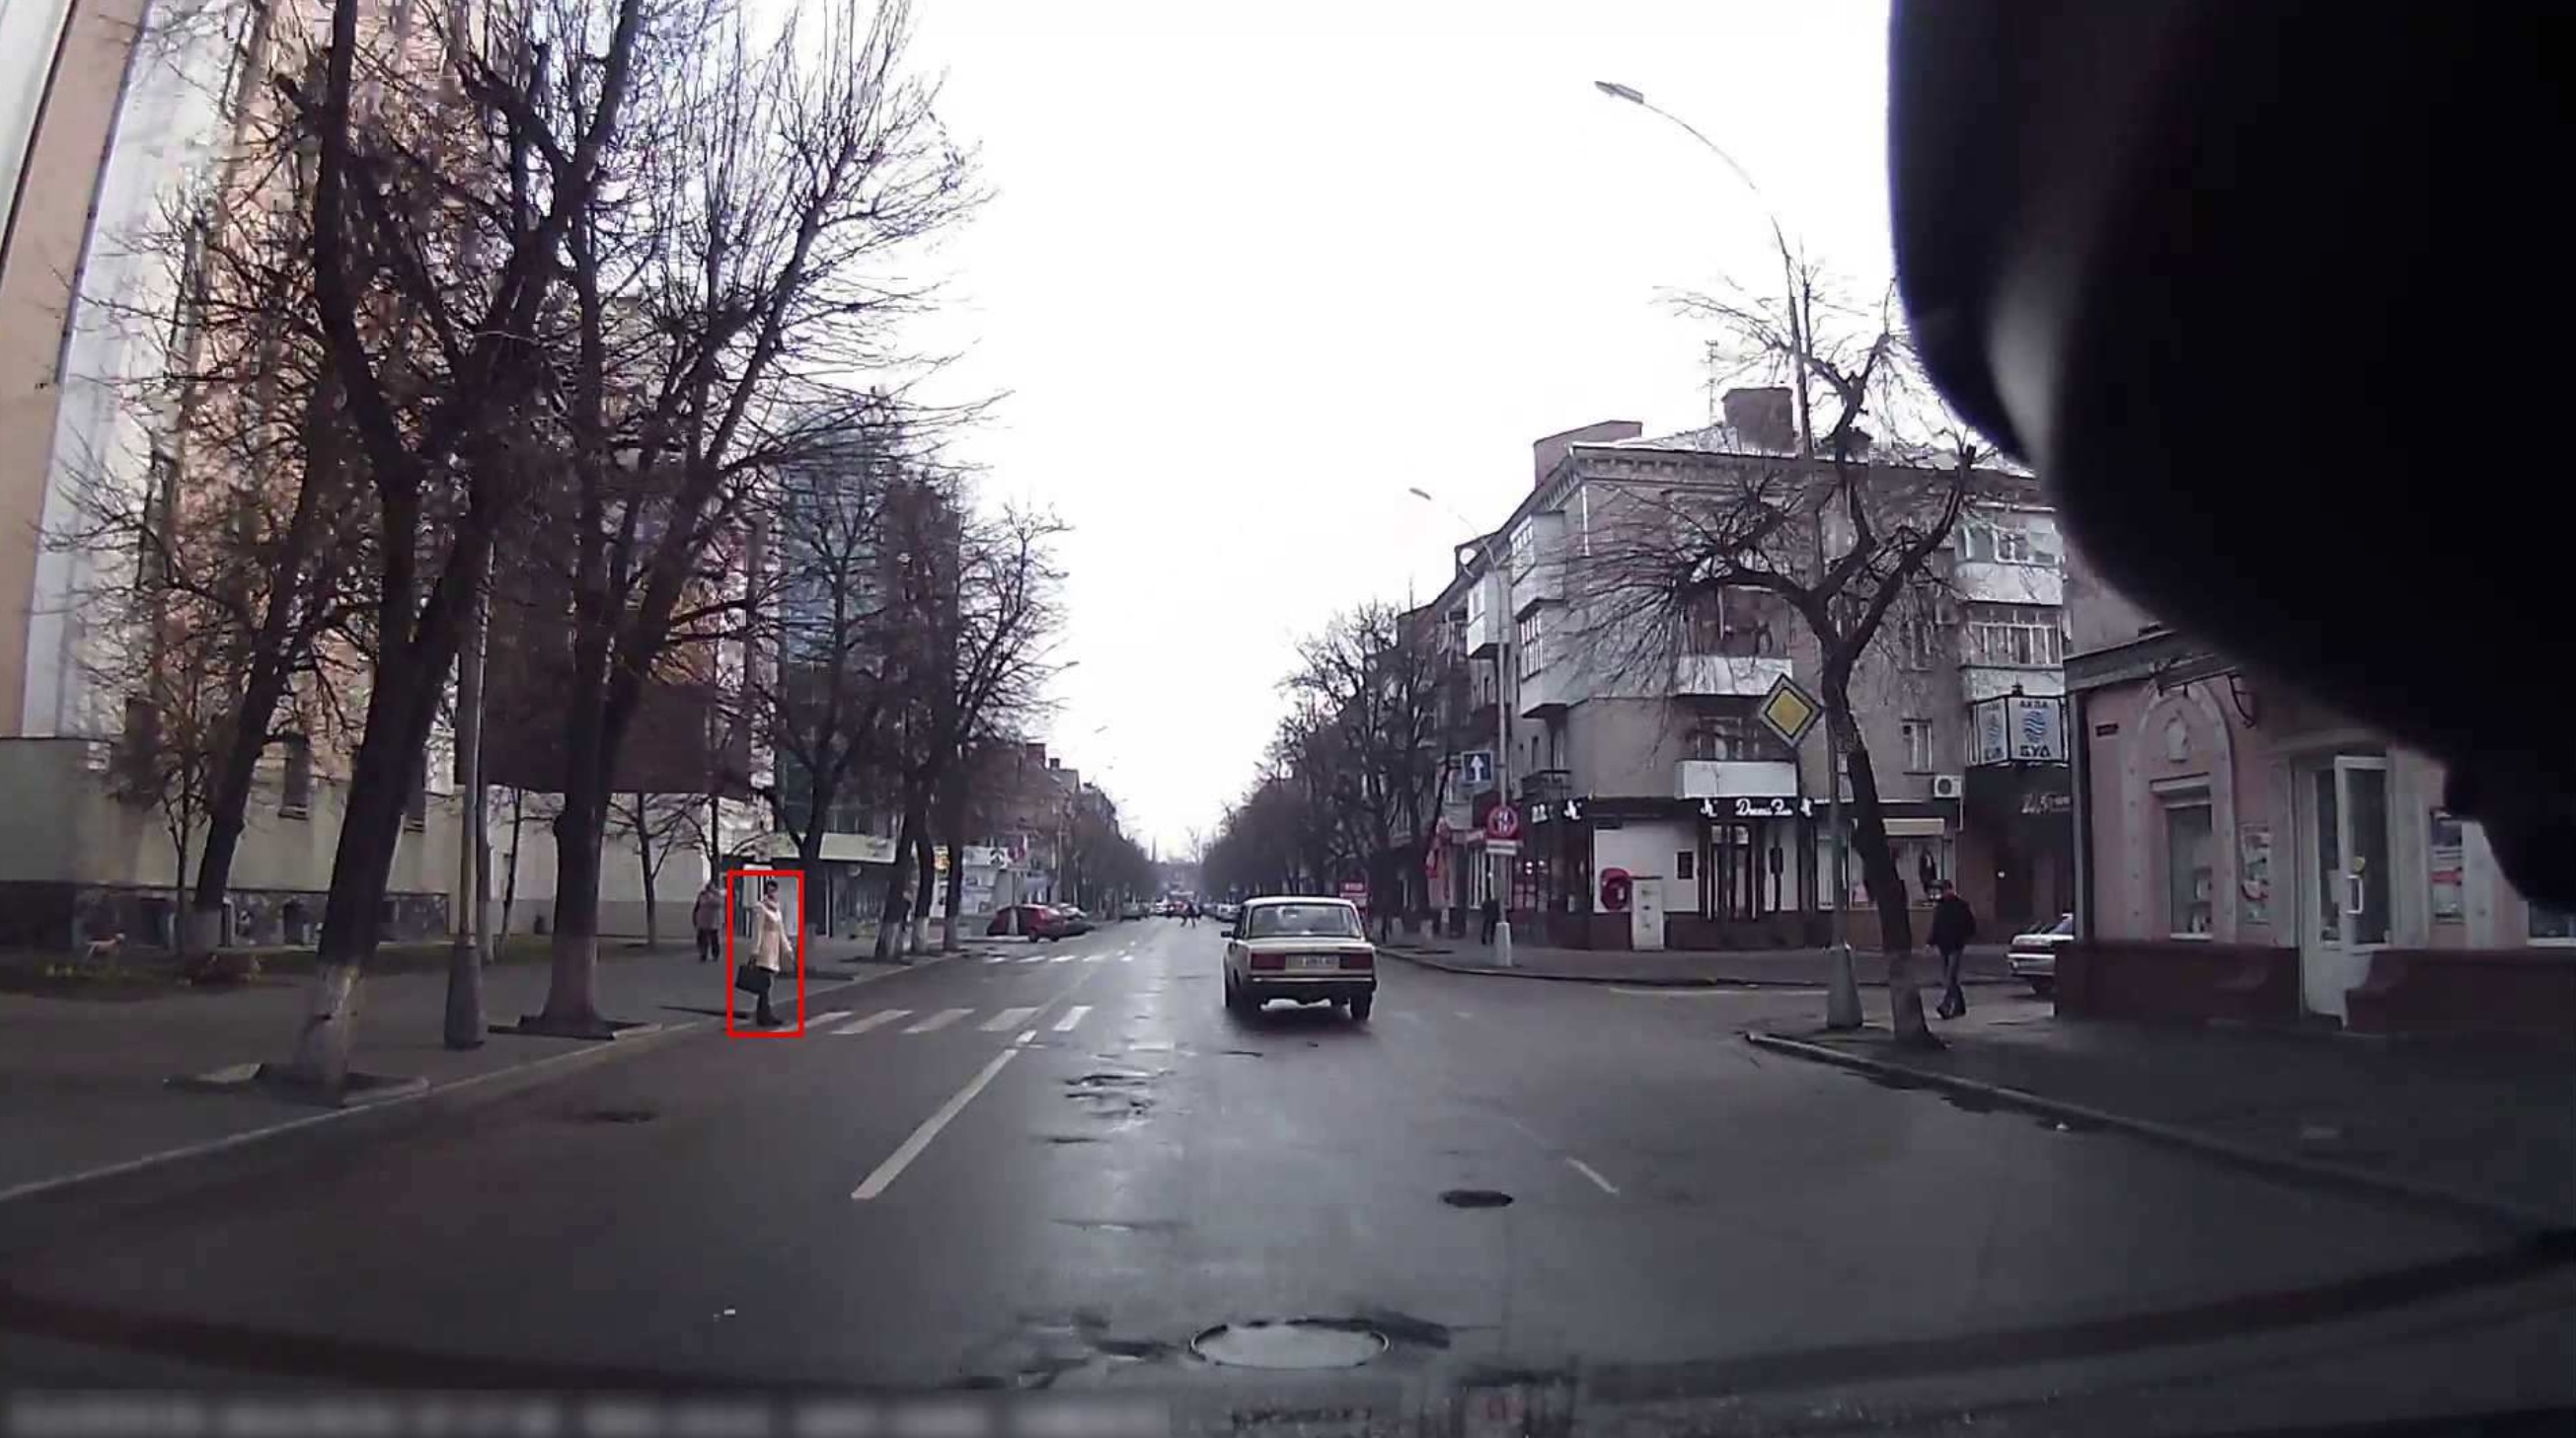
\includegraphics[width=\textwidth]{images/jaad.jpeg}
         \caption{Structured: JAAD}
     \end{subfigure}
     \hfill
     \begin{subfigure}[b]{0.48\textwidth}
         \centering
         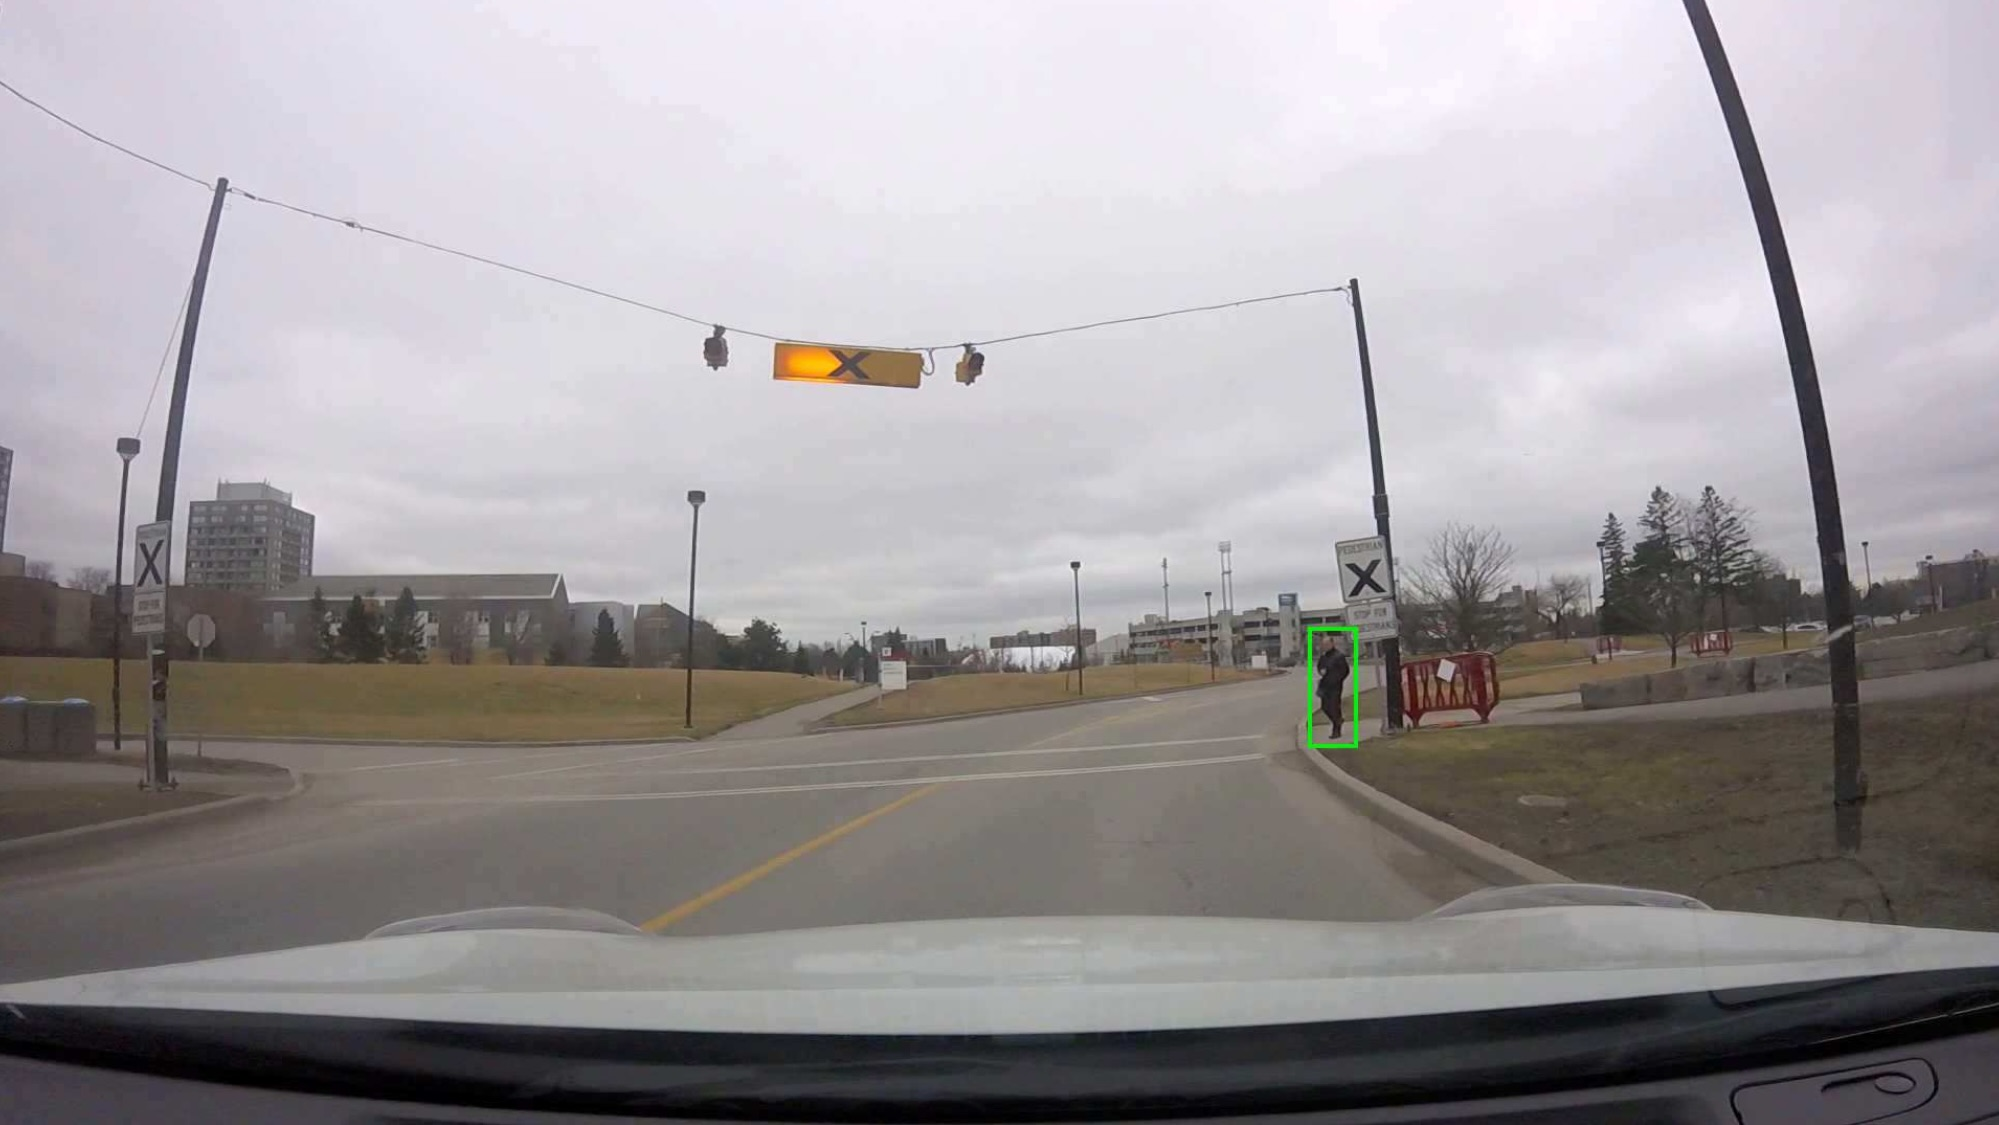
\includegraphics[width=\textwidth]{images/jaad2.jpeg}
         \caption{Structured: PIE}
     \end{subfigure}

     \vspace{1em} % Adds vertical space between rows

     % --- Second Row ---
     \begin{subfigure}[b]{0.48\textwidth}
         \centering
         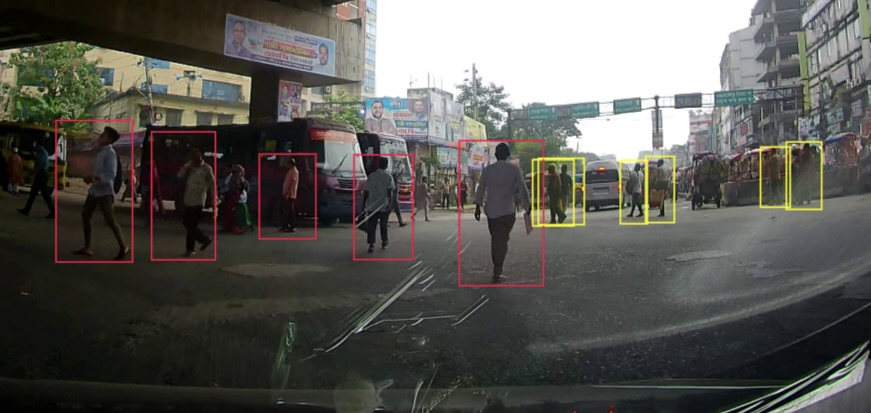
\includegraphics[width=\textwidth]{images/b3.png}
         \caption{Unstructured: BanglaTesla-PeD}
     \end{subfigure}
     \hfill
     \begin{subfigure}[b]{0.48\textwidth}
         \centering
         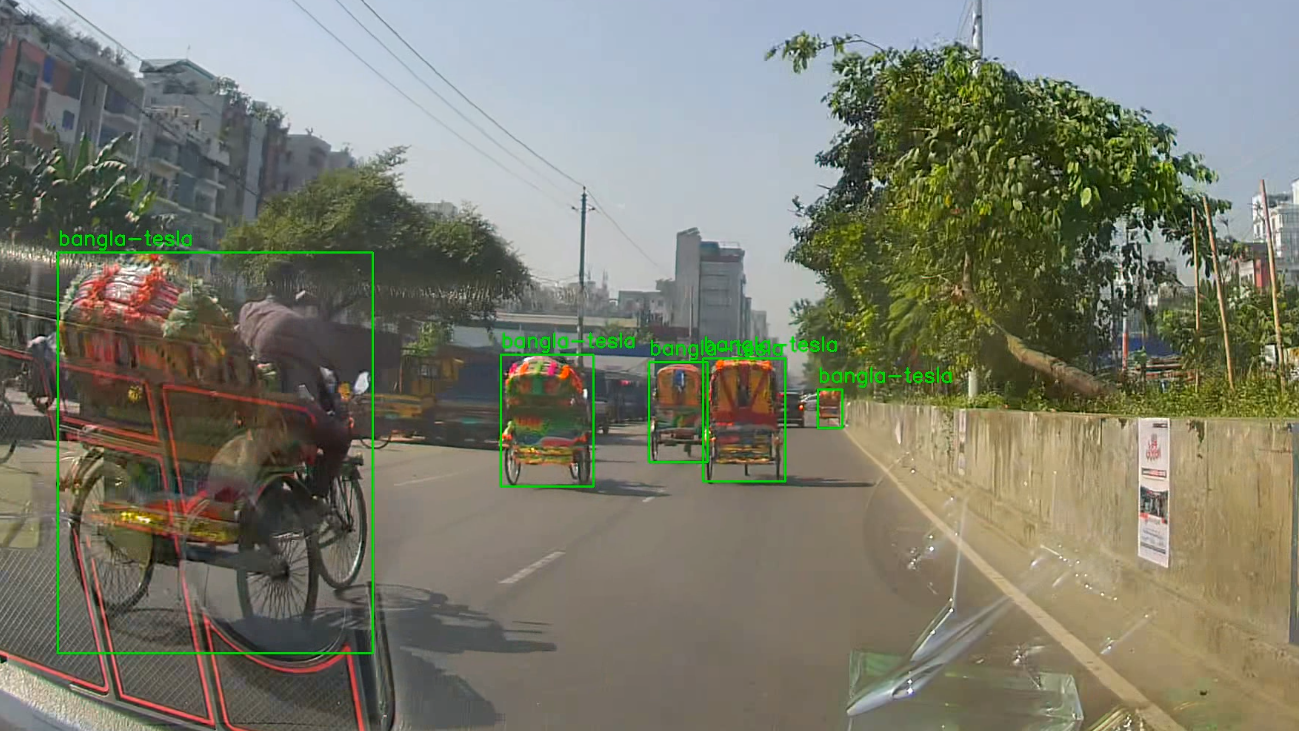
\includegraphics[height=3.8cm, width=\textwidth]{images/Tesla4.png}
         \caption{Unstructured: BanglaTesla-PeD}
     \end{subfigure}

     \caption{Comparison of structured environments (e.g., PIE and JAAD datasets) vs. the unstructured, mixed-traffic environment of Dhaka captured in the BDD-PeD dataset.}
     \label{fig:four_subsystems}
\end{figure}


For instance, in organized settings, a pedestrian waiting at the curb strongly signals an intent to cross only when the signal changes. Pedestrians exhibit "rolling behavior" in chaotic settings \cite{vasudevan2020pedestrian}. They frequently start crossing without a clear right-of-way and change their route and speed to get through traffic. The level of this gap can be measured quantitatively. Modelling/processing, When models that are trained on structured datasets are applied in unstructured settings, such as the one in the IDD-PeD dataset \cite{bokkasam2025pedestrian}, the performance decreases dramatically. The intention prediction accuracy is reduced by up to 15 percent and the error of the trajectory prediction is immense (Mean Squared Error). This decline happens because current models cannot take into account unique environmental factors, such as severe occlusion, uneven lighting, and complex vehicle-pedestrian interactions that are common on South Asian roads.\\

A significant and important gap in current global datasets is the lack of informal electric three wheeler agents. In Dhaka, Bangladesh, the streets are filled with battery-operated three-wheelers, commonly called “BanglaTeslas.” These vehicles share the road with pedestrians, rickshaws, and large vehicles. They show distinct movement patterns. These are high acceleration, quick lane changes, sudden U-turns, and the ability to fit through very narrow spaces. Contrary to ordinary cars or pedestrians, BanglaTeslas operate within a grey zone of the road regulations and mechanics. This poses a special problem in predicting their directions, which is not yet addressed by any available data set, such as the Indian Driving Dataset (IDD-PeD)\cite{bokkasam2025pedestrian}. 

%Unlike regular vehicles or pedestrians, “BanglaTeslas” function in a grey area of traffic rules and physics. This creates a unique challenge in predicting their paths, a problem that no existing dataset, including the Indian Driving Dataset (IDD-PeD) \cite{bokkasam2025pedestrian}, currently solves.

\begin{figure}[h!]
    \centering
    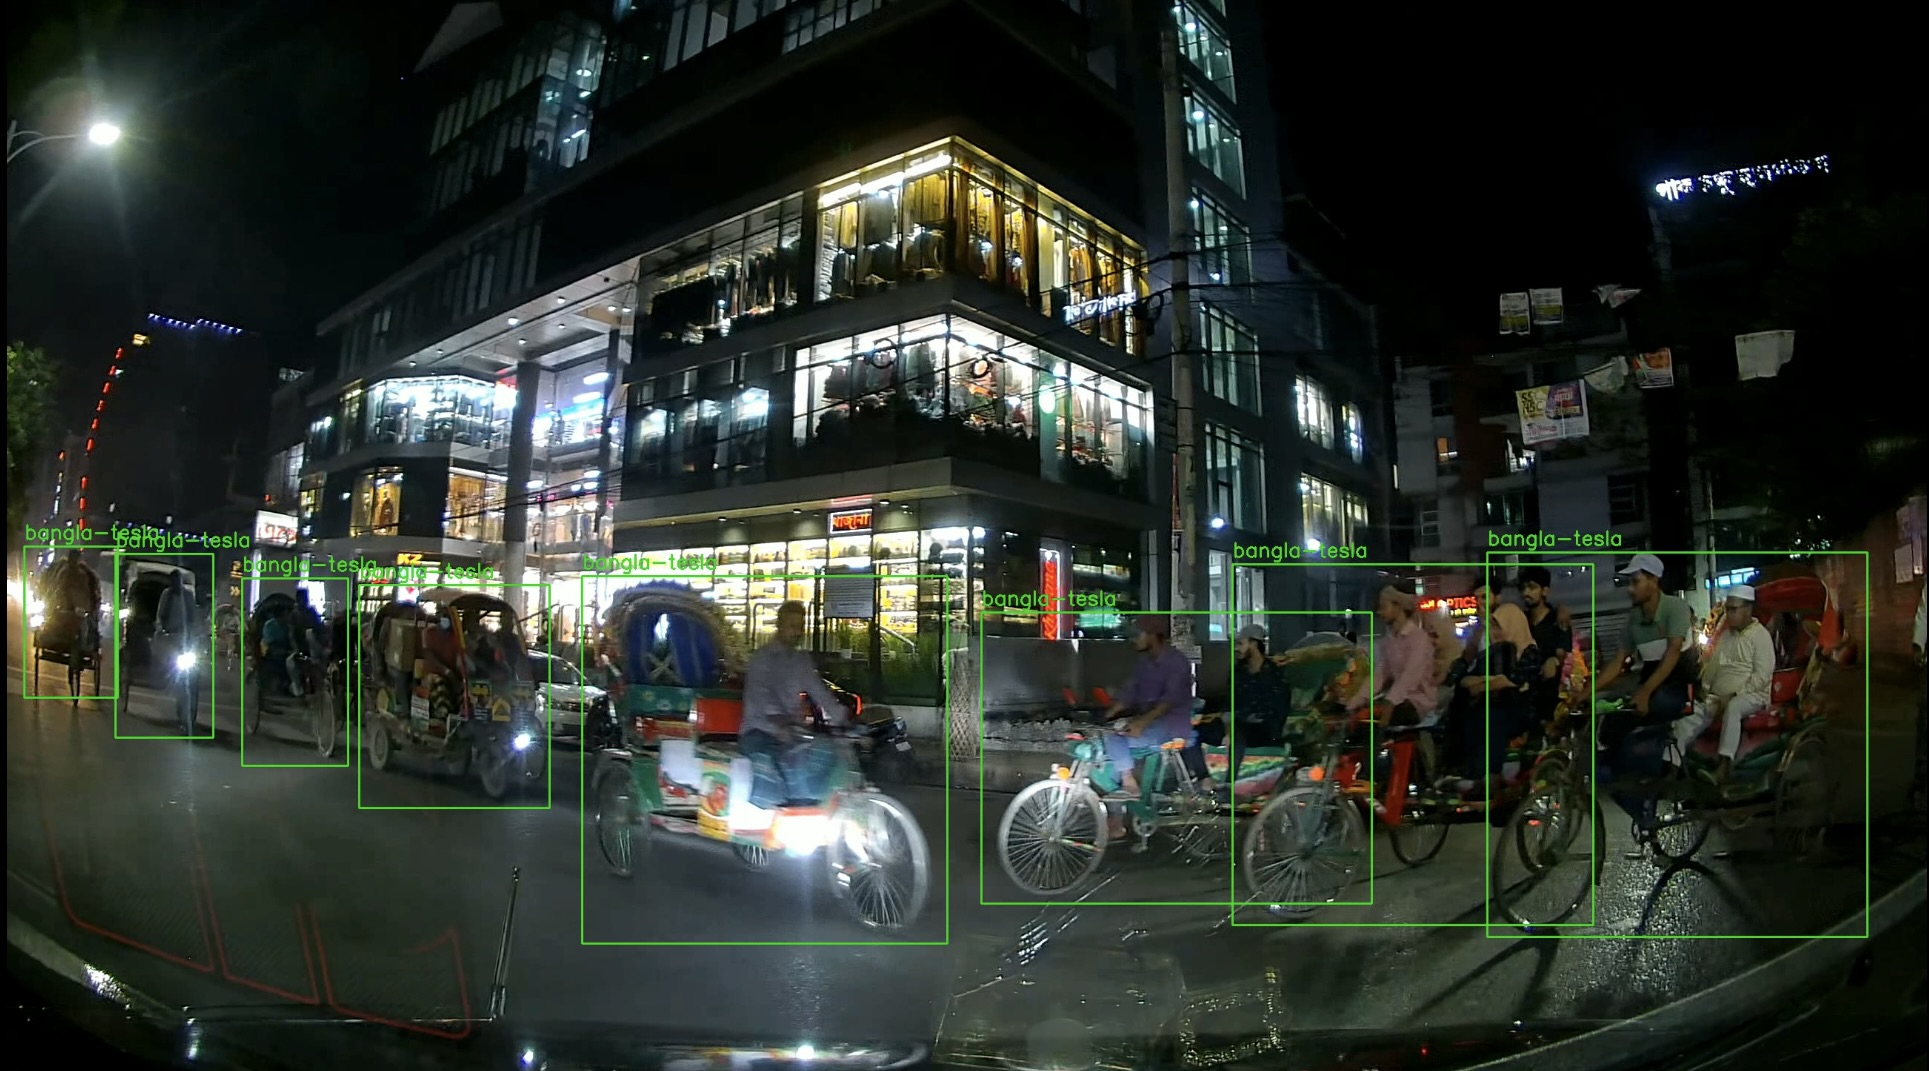
\includegraphics[width=1\textwidth]{images/t1.jpeg} 
    % Uncomment the line above and change the filename to your actual image file
    \caption{The "BanglaTeslas" (Informal Electric Three-Wheelers)}
    \label{fig:bangla-tesla}
\end{figure}


If we consider the prediction of the movements of these common agents to be the major flaw in the functioning of an autonomous vehicle system seeking to operate in Bangladesh, then this could be a huge blind spot.
\vspace{0.5cm}



\subsection{Research Questions}
This research addresses the following key questions regarding the deployment of autonomous perception systems in Bangladesh:

\begin{itemize}
%\item \textbf{RQ1:} To what extent do pedestrian intention and trajectory prediction models trained on structured datasets (IDD-PeD) \cite{bokkasam2025pedestrian} work in the unstructured traffic of Dhaka? 


\item \textbf{RQ1:} How effective are the pedestrian intention and trajectory prediction models that are trained using structured data (IDD-PeD) \cite{bokkasam2025pedestrian} in the unstructured traffic of Dhaka? Previous research has shown that models trained on structured datasets from Western countries tend to struggle when applied in unstructured environments \cite{parikh2024idd}. This struggle occurs due to a lack of lane discipline and non-compliance with traffic signals \cite{vasudevan2020pedestrian}. We examine whether the IDD-PeD dataset, which reflects similar chaotic conditions in India \cite{bokkasam2025pedestrian}, is enough for training models used in Dhaka. We also consider whether the differences in environment require separate adjustments.

\item \textbf{RQ2:} What are the unique behavioral patterns of BanglaTeslas that make them distinct from the general traffic participants and how they impact the prediction accuracy? Currently, western datasets like PIE \cite{rasouli2019pie} and JAAD \cite{rasouli2017are} are centered around the common interactions of vehicles and pedestrians. These electric three-wheelers, BanglaTeslas, display some unique ways of movement. These vehicles demonstrate higher acceleration variability and “rolling behaviors,” \cite{vasudevan2020pedestrian} which are unaligned with the current movement types. Our focus shall be on quantifying the difference within these behaviors to understand their effect on the Mean Squared Error observed for the tasks involving the predictions of the paths.

\item \textbf{RQ3:} Which architectural components and training strategies are most important for improving prediction performance in highly unstructured, mixed-traffic environments? Due to the unpredictable nature of South Asian traffic, we assess whether deterministic methods (e.g., PIETraj \cite{rasouli2019pie}) or stochastic generative models (e.g., SGNet \cite{wang2022stepwise}, BiTraP \cite{yao2021bitrap}) are more effective in predicting traffic. This question will attempt to establish whether it is necessary to model a number of possible futures to be safe in some cases where the adherence to the rules of traffic is not the norm.

\item \textbf{RQ4:} Can one model be useful in predicting the intentions and paths of pedestrians and vehicles in the IDD-PeD and BanglaTesla datasets? Or are their different movement patterns to different models required? In structured setups of autonomous driving, pedestrians as well as vehicles are treated as separate systems. However, the unpredictable interactions of these two groups in Dhaka signal the need for a common model. We dive into the question of whether a single architecture is able to distinguish the irregular latent states of both pedestrians and “BanglaTeslas,” or whether their movement dynamics are too different to be merged.
\end{itemize}

\subsection{Research Objectives}

This study's primary goal is to connect the different autonomous perception capabilities that have been developed for well-structured environments with the total disorder of South Asian roads. The particular research objectives are:

\begin{enumerate}
    \item Testing and optimizing of the basic Pedestrian Intention Prediction (PIP) architectures with the help of the IDD-PeD dataset \cite{bokkasam2025pedestrian}, thereby setting up a high-performance standard for unstructured anthropomorphic environments where traditional motion cues often suffer from occlusion and lack of infrastructure.
    
    \item Gathering and tagging of the ``BanglaTesla'' dataset which consists of a new collection of high-density traffic videos from Dhaka, Bangladesh. The particular aim of this dataset is to include the informal electric three-wheelers (or ``BanglaTeslas'') \cite{jagonews2025banglatesla} that take up local streets but are missing from global datasets like PIE \cite{rasouli2019pie} or Waymo \cite{sun2020scalability}.
    
    \item The estimating of the kinematic divergence of informal vehicular agents (e-rickshaws) through the inspection of acceleration variance, turning radii, and erratic ``rolling behaviors'' \cite{vasudevan2020pedestrian} in relation to regular traffic is being conducted, thus pointing out the reasons why the standard motion models fail to predict their paths accurately.
    
    \item To compare the performance of trajectory prediction models, specifically focusing on the effectiveness of stochastic methods (e.g., SGNet \cite{wang2022stepwise}, BiTraP \cite{yao2021bitrap}) versus deterministic methods in handling the high uncertainty and multimodal nature of local mixed traffic.
    
    \item To create an autonomous driving research baseline in Bangladesh, establishing a quantitative reference for future development of region-specific safety systems and policy-making regarding the integration of informal vehicles into intelligent transport systems \cite{parikh2024idd}.
\end{enumerate}


\subsection{Our Contributions}

In order to overcome the weaknesses of the current autonomous perception systems in the Global South, this paper introduces the following key contributions:

\begin{itemize}
    \item \textbf{Curated BanglaTesla Database:} This is the first dataset to be curated with special attention to the dynamics of the trajectories of informal battery-operated three-wheelers (``BanglaTeslas'') \cite{jagonews2025banglatesla} and pedestrians in Dhaka, Bangladesh. Our dataset, unlike regular datasets which do not consider informal agents \cite{rasouli2019pie, sun2020scalability}, documents high-density, non-compliant traffic behaviors, annotated manually to facilitate autonomous driving research in a specific region.
    
    \item \textbf{State-of-the-Art on IDD-PeD:} We introduce a careful reconsideration and maximization of Pedestrian Intention Prediction (PIP) baselines on the IDD-PeD dataset \cite{bokkasam2025pedestrian}. Our better implementation has an F1 score of 0.83 and an AUC of 0.87, marking a new standard of intention understanding under unstructured settings and greatly outperforming the baseline of the original paper (F1: 0.36).
    
    \item \textbf{Comparison of Stochastic and Deterministic Models:} We present an extensive comparison of trajectory prediction architectures on our new dataset. Compared to deterministic models (e.g., PIETraj \cite{rasouli2019pie}), stochastic models (e.g., SGNet \cite{wang2022stepwise}) are essential to the traffic of Dhaka, and they are the ones that best solve the problem (MSE: 3,872) by modeling multimodal uncertainty.
    
    \item \textbf{Measurement of the Domain Gap:} We make a quantitative determination of the domain gap between Indian (IDD-PeD) \cite{bokkasam2025pedestrian} and Bangladeshi traffic conditions. We show that the error rates in the streets of Dhaka are several orders of magnitude worse than those in IDD-PeD. This points to the fact that the applicability of the concept of the ``BanglaTeslas'' has a unique kinematic complexity, which can be used as a baseline to develop future safety systems in the area.
\end{itemize}


\subsection{Report Structure Overview}
The report is structured in a way that gives a clear guidance towards application of theoretical knowledge of deep learning and computer vision to real life problems. This paper (Section 2) reviews the literature available on predicting pedestrian intentions and trajectories. It makes a comparison between techniques suited to structured Western settings and new requirements of unstructured ones. Section 3 describes our research methodology. It includes the process of curating and annotating the BanglaTesla dataset along with the specifications of the stochastic and deterministic models that we employ. The results of the experiment are provided in Section 4. It offers a quantitative study in-depth comparison of baseline performances on the IDD-PeD dataset and the preliminary analysis of our new dataset. In the 5th section we give a significant discussion of the experiment outcomes. It studies failure concerns of both environmental and kinematic divergence. Then, Section 6 grants the restrictions and future assignments in CSE499B. Lastly, Section 7 provides a report summary and reflects on the overall impact of the work on autonomous perception in the Global South.



\clearpage
\section{Literature Review}

\subsection{Key Concepts \& Related Work}
The field of autonomous perception has changed a lot, going from basic object detection to advanced behavioral forecasting. This section looks at the development of datasets and methods in Pedestrian Intention Prediction (PIP) and Trajectory Prediction (PTP). Additionally, it also points out the differences between Western baselines and new, unstructured benchmarks.

\subsubsection{Evolution of Datasets: From Structured to Unstructured}
Early research in pedestrian behavior was driven by datasets captured in highly regulated environments. JAAD \cite{rasouli2017are} and PIE \cite{rasouli2019pie} played a key role in setting standards for predicting intentions. They concentrated on interactions at marked crosswalks and signalized intersections in Western countries like North America and Europe. Likewise, the Waymo Open Dataset \cite{sun2020scalability} offered high-resolution sensor data for autonomous driving. But, in most of its scenarios, the compliant road users were mainly the ones who obeyed the lane rules. Still, the limitations of these datasets were very evident in the case of South Asian countries like Bangladesh and India. With the help of the TITAN dataset \cite{malla2020titan}, very interactive scenarios were given, but confined to organized urban environments only. With this gap in place, recent literature has started to center attention to unstructured settings. IDD-X cite{parikh2024idd} and IDD-PeD \cite{bokkasam2025pedestrian}, were developed to record the unique chaotic traffic available in the Indian roads, which is full of non-compliant pedestrians and without lane markings. IDD-PeD, in particular, provides the largest collection of annotated pedestrian bounding boxes in unstructured settings and serves as the main baseline for this study.

\subsubsection{Pedestrian Intention Prediction (PIP)}
PIP mainly works as a binary classification task. It decides if a pedestrian will cross the street or not. Early methods depended on static visual signals like head orientation and body pose. Now, more detailed models use spatio-temporal methods. For example, I3D (Inception-3D) and ConvLSTM models have become popular for capturing motion features from video clips \cite{bokkasam2025pedestrian}. Rasouli et al. \cite{rasouli2019pie} showed that adding context, such as vehicle speed and traffic light status, greatly increases intention accuracy. However, these contextual signals are often missing or irrelevant in unstructured environments where traffic signals are ignored. This makes it necessary for models to focus more on different motion dynamics.

\subsubsection{Trajectory Prediction: Deterministic vs. Stochastic}
Trajectory prediction aims to forecast the future coordinates of an agent based on past observations. Approaches fall into two categories:

\begin{itemize}
    \item \textbf{Deterministic Models:} Methods like PIETraj \cite{rasouli2019pie} predict a single ``most likely'' future path. While they are efficient, they struggle in situations with high uncertainty because they cannot account for the multiple choices people might make.
    
    \item \textbf{Stochastic Models:} Recognizing that a pedestrian may choose several valid paths, generative models have become more popular. BiTraP \cite{yao2021bitrap} uses a bi-directional LSTM with a Conditional Variational Autoencoder (CVAE) to create several plausible trajectories. Similarly, some popular architectures like SGNet (Stepwise Goal-Driven Networks) \cite{wang2022stepwise} and Multimodal Transformer Networks \cite{yin2021multimodal} clearly model long-term goals to improve intermediate steps. These stochastic approaches are thought to be more effective in chaotic environments where ``rolling behavior'' \cite{vasudevan2020pedestrian} leads to ongoing uncertainty.
\end{itemize}

\subsection{Identification of Gaps in Current Research}
There are still important gaps when applying these architectures to the specific context of Bangladesh. This is true even with the successes in behavioral prediction.

\subsubsection{The ``Unstructured'' Definition Gap}
Datasets such as IDD-PeD \cite{bokkasam2025pedestrian} do cover unstructured traffic but they mainly translate ``unstructured'' through the Indian traffic conditions perspective. The context is much alike in Bangladesh but Indian datasets do not cover the particular kinematic trajectory of battery-powered three-wheelers, nicknamed ``BanglaTeslas.'' These vehicles possess distinctive acceleration patterns and turning radii, they are different from Indian auto-rickshaws or Western vehicles like sedans. As of now, there is no dataset that illustrates the trajectory dynamics of these informal agents \cite{sun2020scalability}.

\subsubsection{Failure of Generalization}

The existing literature emphasizes that there is a high level of performance decay when models trained on structured data are used on unstructured ones. According to Vasudevan et al. \cite{vasudevan2020pedestrian}, there are significant differences in the nature of pedestrian gap-acceptance behavior in South Asia as opposed to the Western models. In South Asia, pedestrians practice ``rolling gap acceptance,'' where they merge into traffic instead of waiting for a clear gap. Current deterministic models based on JAAD or PIE do not consider this ongoing negotiation. As a result, they have high False Negative rates in collision warning systems \cite{katyal2020intent}.

\subsubsection{Lack of Region-Specific Benchmarks}
There is a clear lack of quantitative comparison for autonomous perception in Bangladesh. While there are general studies on computer vision, no research has thoroughly tested the performance of stochastic and deterministic trajectory models on the mixed traffic in Dhaka. As a result, we do not know if architectures like SGNet \cite{wang2022stepwise} or BiTraP \cite{yao2021bitrap} can manage the high density and occlusion common on Dhaka's roads without specific changes. This study aims to fill this gap by creating the ``BanglaTesla'' dataset and offering the first comparative analysis of these architectures in this unique setting.


%\section{Methodology}
%
%\subsection{Research Design}
%This research employs a quantitative experimental design centered on a machine learning pipeline. The main goal is to assess how well trajectory prediction models adapt when moving from the unstructured but similar traffic in India (IDD-PeD) \cite{bokkasam2025pedestrian} to the varied and extremely dense traffic in Dhaka. The three stages of the research process are the dataset curation, baseline model optimization, and pipeline for comparative evaluation.
%
%\subsubsection{Phase 1: Dataset Curation (The ``BanglaTesla'' Dataset)}
%To address the lack of domain-specific data, we implement a primary data collection phase. High-definition video data is captured from ego-centric perspectives on major thoroughfares in Dhaka. The research methodology specifically aims to capture ``edge cases'' that are not included in Western datasets like JAAD \cite{rasouli2017are} and PIE \cite{rasouli2019pie}, such as rolling pedestrian crossings, aggressive lane-splitting, and electric ``BanglaTesla'' three-wheelers \cite{jagonews2025banglatesla}. These videos undergo manual annotation to generate ground-truth trajectories and bounding boxes compatible with standard formats.
%
%\subsubsection{Phase 2: Training Approach \& Algorithmic Framework}
%In order to investigate our research questions, the experimental setting compares two different modeling paradigms:
%
%\begin{itemize}
%    \item \textbf{Deterministic Framework:} To illustrate common single-trajectory forecasting techniques, we use PIETraj \cite{rasouli2019pie} as the baseline. Additionally, this tests the theory that chaotic systems cannot be well predicted by a single path.
%    \item \textbf{Stochastic Framework:} We use the SGNet \cite{wang2022stepwise} and BiTraP \cite{yao2021bitrap} architectures to illustrate generative methods. These models could better handle the ``rolling behavior'' of local agents by using Conditional Variational Autoencoders (CVAEs) to anticipate many potential futures.
%\end{itemize}
%
%\subsubsection{Phase 3: Evaluation Pipeline}
%The research employs a Transfer Learning strategy. Models are first pre-trained on the large-scale IDD-PeD dataset \cite{bokkasam2025pedestrian} to learn general unstructured motion features. Then it is fine-tuned on the ``BanglaTesla'' dataset to adapt to local kinematic nuances. The design uses a split-sample validation strategy (70\% training, 15\% validation, 15\% testing). Performance is quantified using standard Euclidean metrics—Average Displacement Error (ADE) and Final Displacement Error (FDE)—along with intention classification metrics (F1-Score, AUC). The ``Domain Gap Analysis,'' a crucial part of the design, measures the performance degradation brought on by the unique kinematics of informal actors by testing models trained exclusively on IDD-PeD on Dhaka data.
%
%
%\subsection{Tools \& Technologies}
%
%The proposed research pipeline uses a strong set of open-source software and hardware acceleration tools. The main development environment is based on Python 3.8 or higher. This choice comes from its wide range of machine learning libraries.
%
%\begin{itemize}
%    \item \textbf{Deep Learning Frameworks:} Model training and inference are done with PyTorch. This library offers dynamic computational graphs. This is important for the complex spatio-temporal structures such as SGNet and BiTraP. We also used TorchVision for image preprocessing and NumPy for efficient matrix operations when handling trajectory data.
%
%    \item \textbf{Data Annotation \& Processing:} To create the ``BanglaTesla'' dataset, we use CVAT (Computer Vision Annotation Tool). This web-based tool allows for manual annotation of bounding boxes and track IDs needed for ground-truth generation, frame by frame. We handle video preprocessing, such as frame extraction and resolution normalization, with OpenCV.
%
%    \item \textbf{Hardware Acceleration:}  The computational demands of training are mostly Generative Adversarial Networks (GANs) and Transformer-based models. All experiments are done on a personal computer setup with an NVIDIA GeForce RTX 3060 GPU (12GB VRAM) and CUDA 13.1 and CuDNN 9.1 libraries are used to improve parallel processing speed during training.
%
%    \item \textbf{Evaluation \& Visualization:}  We calculate quantitative metrics (ADE/FDE) using custom scripts. We use Matplotlib and Seaborn to create visual plots for trajectory divergence and loss convergence. We manage code versioning and collaboration through GitHub, which helps ensure we can reproduce the experiments.
%\end{itemize}
%
%
%\subsection{Data Collection \& Preparation}
%This research makes use of two different datasets to thoroughly assess the domain gap between general unstructured traffic and the unique kinematic problems of Dhaka. Initially, baseline models on unstructured environments are trained using IDD-PeD as the source domain. The second is our unique "BanglaTesla" Dataset, which is the target domain for optimizing and assessing performance in Bangladesh's extremely congested, unofficial traffic.
%
%
%\subsubsection{IDD-PeD Dataset (Baseline)}
%
%For the first level of training, we use the \textbf{Indian Driving Dataset – Pedestrian (IDD-PeD)} \cite{bokkasam2025pedestrian}. We chose IDD-PeD because it was the only large-scale public benchmark available that approximated the unstructured road scenarios common to South Asia and included the necessary parameters of illumination changes and unsignalized crossings.
%
%\begin{itemize}
%    \item \textbf{Data Collection Setup:} The data is comprised of more than 100 hours of driving videos using two ego-mounted front-facing cameras, namely a GoPro Hero 8 Black with a resolution of 30 FPS and a DDPAI X2SPro with a resolution of 25 FPS in HD resolution. Additionally, ego-motion data was collected using the OBD sensor, which was synchronized with the cameras and yielded a resolution of 10 Hz \cite{bokkasam2025pedestrian}.
%
%    \item \textbf{Environmental Diversity:} The data were collected from urban areas with high population densities across South Asia, resulting in a diversity of pedestrian behaviors under chaotic situations. The scenarios are also quite diverse, ranging from unpaved commercial roads to residential streets, including both day and night lightings.
%
%    \item \textbf{Dataset Organization and Split:} The dataset consists of high-definition videos split into nine separate sets (\texttt{gp\_set\_0001} to \texttt{gp\_set\_0009}). The standard split pattern for this dataset consists of training on sets 1, 2, 4, 6, and 7, while sets 3, 5, 8, and 9 are for testing, which makes a rough split of 70\% training and 30\% testing. The training split has 3,284 people, and for testing, there are 1,632 people.
%
%    \item \textbf{Multi-Level Annotation Schema:} Unlike other datasets that are annotated only by rectangles, IDD-PeD is annotated at five levels that address the complexity involved in unstructured traffic \cite{bokkasam2025pedestrian}:
%    \begin{enumerate}
%        \item \textbf{Spatial Annotations:} Using bounding boxes, where the occlusion level is categorized as None, Partially Occluded, and Fully Occluded, and 2D Pose Annotations, which include 17 keypoints of the human body and are obtained by MMPose.
%        \item \textbf{Behavioral Annotations:} Hierarchical, frame-level attributes grouped into six classes. Of foremost interest for HDMAP-related work are non-compliant behaviors such as ``Weaving Through Traffic (WTT)'' (drivers weaving between slower-moving vehicles) and ``Looking Over Shoulder (LOS)'' (a primary intention-behavior indicator, independent of hand or head movement).
%        \item \textbf{Interaction Annotations:} Binary variables that highlight interactions where the pedestrian explicitly affects the trajectory of the ego vehicle.
%        \item \textbf{Scene Annotations:} These are scene-level annotations, including environment descriptions such as Intersection Type (T-right, Y-intersection, etc.) and Signalized Type (Crosswalk, Traffic Signal).
%        \item \textbf{Location Annotations:} Spatial context markers putting the pedestrian in the context of the road infrastructure (e.g., ``Near Divider,'' ``Side of the Road'').
%    \end{enumerate}
%
%    \item \textbf{Data Statistics:} Data statistics show that the median ego-car speed and the median track length of the pedestrian path are 30 km/h and 60 frames, respectively. Notably, it offers a lot of data on ``rolling behavior,'' where pedestrians momentarily hesitate before continuing to cross \cite{bokkasam2025pedestrian}.
%\end{itemize}
%
%
%\subsubsection{BanglaTesla Dataset (Novel Target)}
%
%To address the significant absence of informal, battery-operated three-wheelers in existing global autonomous driving standards, we propose the \textbf{``BanglaTesla'' Dataset}. Modeled on the rigorous structure of IDD-PeD \cite{bokkasam2025pedestrian}, this dataset has been specifically developed to capture the complex interplay between pedestrians and informal vehicular agents, a dynamic that dominates the hyper-dense roads of Dhaka.
%
%\begin{itemize}
%    \item \textbf{Data Collection Setup:} The dataset comprises high-definition video footage (1080p at 30 fps) captured using ego-centric dashboard cameras. Data collection focused on the most congested thoroughfares of Dhaka, specifically \textbf{Mirpur, Farmgate, and Mohakhali}, which are known for their extreme traffic density. Unlike IDD-PeD, which represents a broad spectrum of general Indian traffic, our setup was engineered to capture ``edge cases'' specific to the Bangladeshi context \cite{baig2024badodd}. This primarily involves the aggressive maneuvering of electric three-wheelers, which are often underrepresented in general datasets.
%
%    \item \textbf{``BanglaTesla'' Agent Taxonomy:} A core contribution of this corpus is the distinct classification of the \textbf{``BanglaTesla'' (Electric Three-Wheeler)}. While other datasets often aggregate three-wheelers into a generic ``Auto-Rickshaw'' category, this research isolates the agent to analyze its unique kinematic profile \cite{hossain2023affordable}. These vehicles are defined by:
%    \begin{itemize}
%        \item \textbf{High Acceleration Variance:} The electric powertrain delivers instant torque, allowing for rapid acceleration and braking maneuvers that differ significantly from combustion-engine counterparts \cite{hossain2023affordable}.
%        \item \textbf{Near-Zero Turning Radii:} These vehicles possess the ability to execute tight U-turns within narrow road corridors, creating unpredictable trajectory deviations.
%        \item \textbf{Silent Operation:} The lack of engine noise significantly impacts pedestrian situational awareness and reaction times compared to conventional vehicles, increasing collision risk \cite{jagonews2025banglatesla}.
%    \end{itemize}
%
%    \item \textbf{Multi-Level Annotation Schema:} Using the \textbf{CVAT (Computer Vision Annotation Tool)}, we applied a multi-level annotation schema that extends the IDD-PeD format to support region-specific behaviors:
%    \begin{enumerate}
%        \item \textbf{Spatial Annotations:} We generated frame-by-frame tight bounding boxes for pedestrians and ``BanglaTeslas.'' Consistent with IDD-PeD, occlusion levels (None, Partial, Full) were annotated to quantify the high degree of visual clutter present in Dhaka's traffic \cite{bokkasam2025pedestrian}.
%        \item \textbf{Trajectory Tracking:} Unique \textbf{Track IDs} were assigned to all agents to capture temporal movement patterns over sequences of 3--5 seconds, facilitating long-term trajectory prediction analysis.
%        \item \textbf{Behavioral Characteristics:} We introduced region-specific behavioral labels absent in international datasets:
%        \begin{itemize}
%            \item \textbf{``Lane Splitting'':} Annotated for vehicular entities aggressively maneuvering between established lanes.
%            \item \textbf{``Rolling Gap Acceptance'':} A phenomenon frequently observed in Dhaka where pedestrians merge into the traffic stream without waiting for a clear gap \cite{vasudevan2020pedestrian}.
%        \end{itemize}
%        \item \textbf{Interaction Annotations:} Binary flags indicating ``Evasive Maneuvers,'' identifying instances where the ego-vehicle or a ``BanglaTesla'' was forced to alter its trajectory in response to erratic pedestrian conduct.
%        \item \textbf{Scene Context:} Annotations classifying specific unstructured road environments, such as ``Unmarked Intersection,'' ``Mid-block Jaywalking Zone,'' or ``Informal Bus Stop.''
%    \end{enumerate}
%
%    \item \textbf{Data Statistics:} The dataset captures high-density interactions in scenarios where the ego-vehicle speed fluctuates continuously between 0--40 km/h. A significant portion of the data focuses on unsignalized junctions, as these account for the predominant proportion of conflict points in Dhaka's environment \cite{baig2024badodd}.
%\end{itemize}
%
%
%
%\subsubsection{Comparative Data Statistics and Kinematic Analysis}
%
%To effectively measure the ``domain gap'' concept, this research performs a comparative statistical analysis between the base IDD-PeD dataset and the target BanglaTesla dataset. In the analysis, the growing complexity in moving from general unstructured traffic to the hyper-dense and unplanned city environment of Dhaka is highlighted.
%
%\begin{itemize}
%    \item \textbf{Volume and Composition of Data:} The baseline of IDD-PeD is quite large, with 205,145 labeled frames and 5,000 unique pedestrian tracks \cite{bokkasam2025pedestrian}. The average length of the tracks is 60 frames (approximately 2 seconds), resulting in moderate temporal information. By contrast, the total number of labeled frames of the BanglaTesla dataset is [N] with [N] unique tracks and [N] BanglaTesla trajectories. These counts are enough for obtaining significant results when fine-tuning deep neural networks on the task domain.
%
%    \item \textbf{Kinematic Profile (Velocity and Acceleration):} IDD-PeD shows smoothly varying ego vehicle velocity, with a median velocity of 30 km/h \cite{bokkasam2025pedestrian}. Although unorganized, the traffic pattern consists mainly of gasoline-powered vehicles with predictable acceleration. An important aspect, which distinguishes the BanglaTesla, lies within the kinematic profile of the vehicles. Observations show that the acceleration distribution of the BanglaTesla vehicles follows a bi-modal distribution, with highly frequent acceleration spikes of more than 2.5 $m/s^2$, thereby validating the assumption that the electric vehicles are drastically different from the auto-rickshaws associated with IDD-PeD \cite{hossain2023affordable}.
%
%    \item \textbf{Interaction Density:} Interaction density is measured by the number of conflicts per minute. IDD-PeD has a high level of interaction density compared to Western data. There is a large number of incidents of jaywalking and weaving \cite{bokkasam2025pedestrian}. The BanglaTesla data has an interaction density of [N] interactions per minute. This is substantially higher compared to IDD-PeD. Additionally, this is higher by multiple orders of magnitude compared to PIE \cite{rasouli2019pie}.
%
%    \item \textbf{Occlusion Levels:} Occlusion is one of the most challenging situations in unstructured environments. In IDD-PeD, it has been observed that about 12\% of the labeled data are totally occluded, and 7\% of data are partially occluded \cite{bokkasam2025pedestrian}. In BanglaTesla, the scenario of occlusion is more intense because of the high density of three-wheelers; [X]\% of pedestrian tracks are partially occluded, while [Y]\% of tracks are totally occluded for at least 20\% of their average duration. Such a scenario provides a tough environment for assessing the robustness of trajectory prediction models, including SGNet.
%\end{itemize}


\clearpage
\section{Methodology}

\subsection{Research Design}
The study utilizes a machine learning pipeline as the foundation for a quantitative experimental design. The primary purpose is to evaluate the adaptability of the trajectory prediction models in transitioning from the disorganized yet comparable traffic of India (IDD-PeD) \cite{bokkasam2025pedestrian} to the diverse and very congested traffic of Dhaka. The research process consists of three phases which are: data collection, baseline model calibration, and comparative evaluation pipeline.


\begin{figure}[h!]
    \centering
    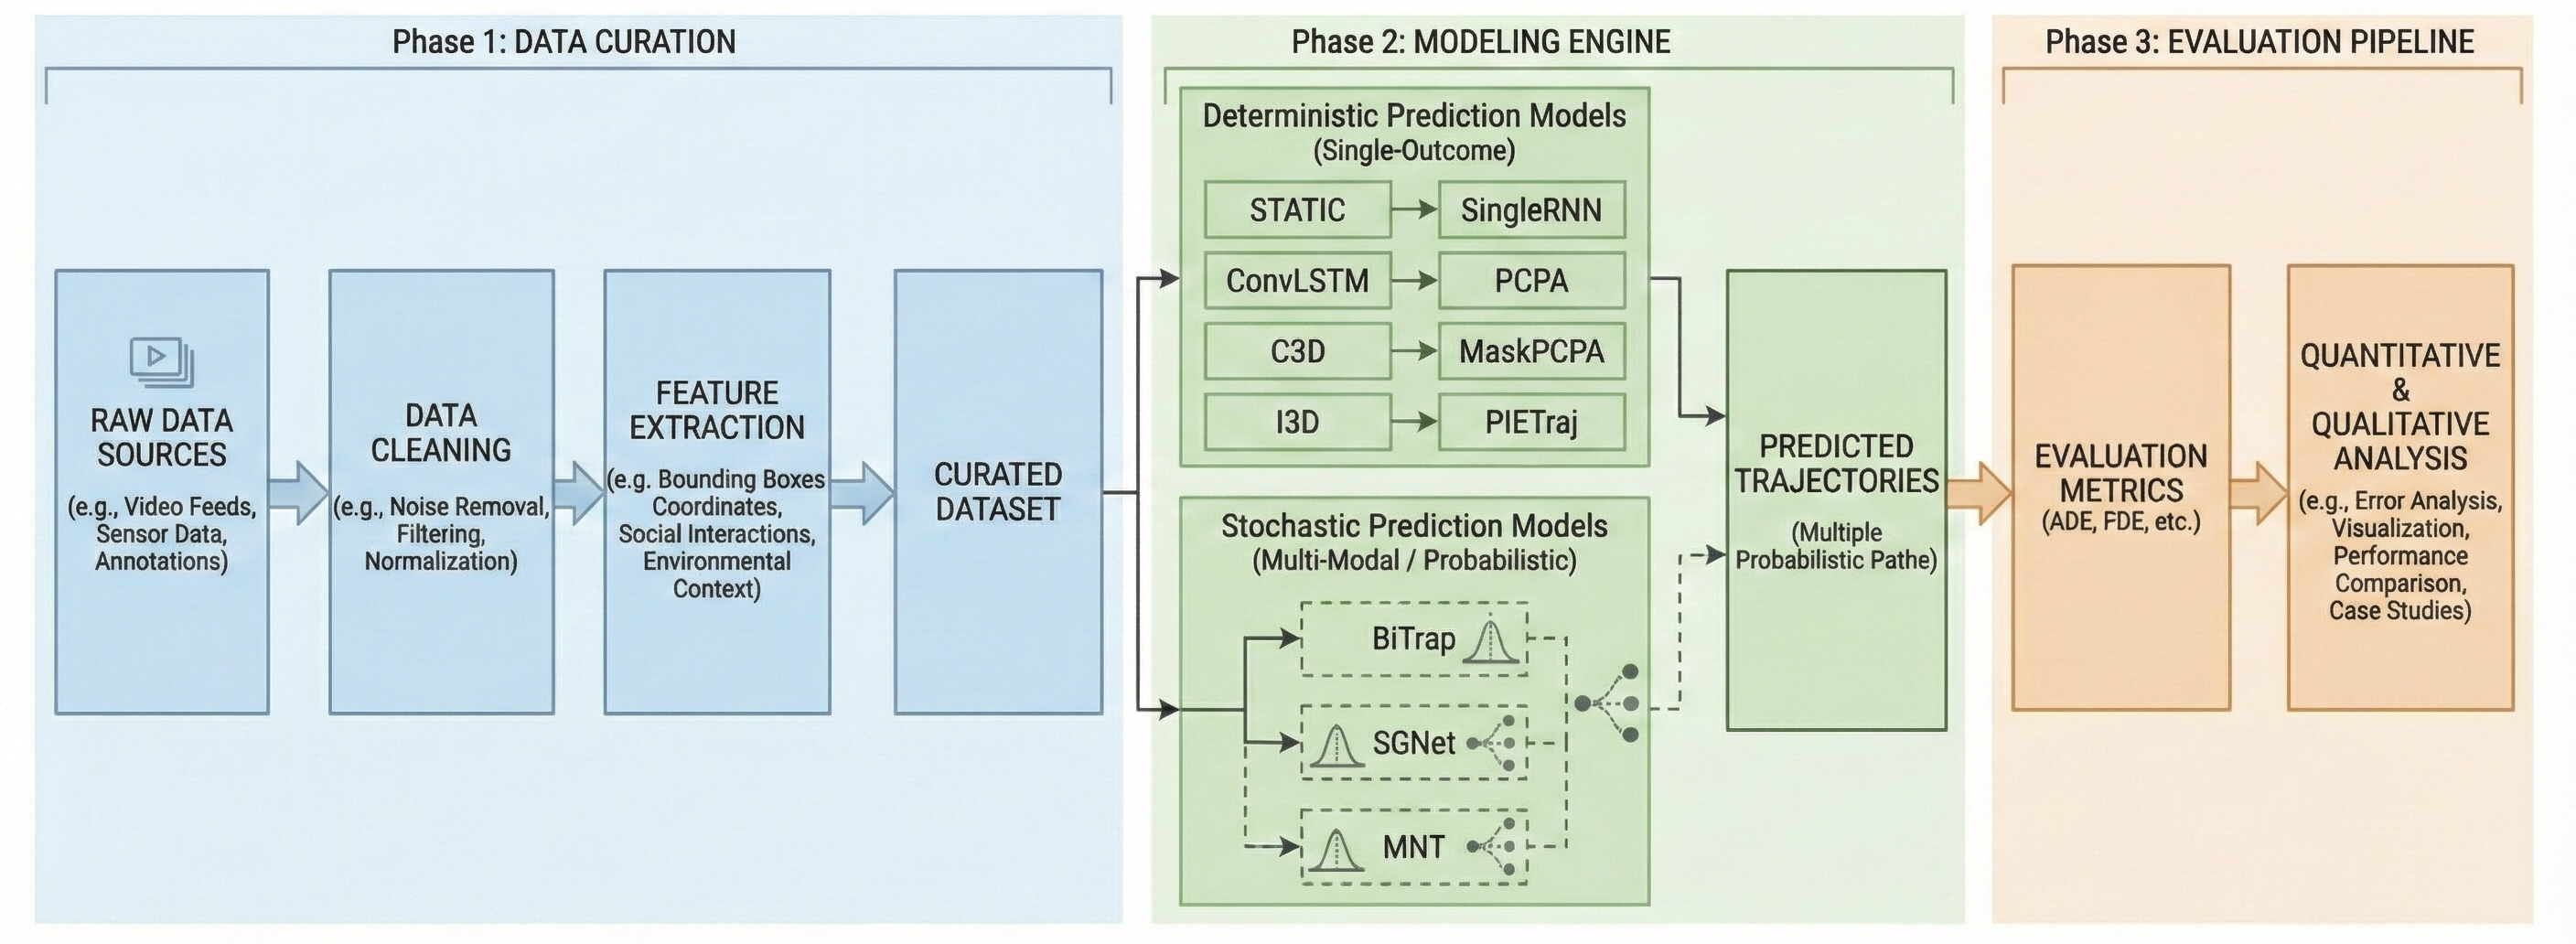
\includegraphics[width=1\textwidth]{images/h-pipeline.jpeg} 
    % Uncomment the line above and change the filename to your actual image file
    \caption{The proposed Research Pipeline. Phase 1 involves Data Curation; Phase 2 Involves Modeling Engine: Stochastic and Deterministic; Phase 3 involves the Evaluation Pipeline.}
    \label{fig:use_case}
\end{figure}

\subsubsection{Phase 1: Dataset Curation (The ``BanglaTesla'' Dataset)}
In order to overcome the issue of insufficient data specific to the domain, we plan to carry out a primary data collection stage. It is the main roads in Dhaka where video data is recorded by taking high-definition ego-centric viewpoints. The methodology of the research is designed to capture situations that are not encountered in Western datasets such as JAAD \cite{rasouli2017are} and PIE \cite{rasouli2019pie} (rolling pedestrian crossings, aggressive lane-splitting, and electric ``BanglaTesla'' three-wheelers \cite{jagonews2025banglatesla}). The videos are then manually annotated to produce ground-truth trajectories and bounding boxes that can be used with standard formats.

\subsubsection{Phase 2: Training Approach \& Algorithmic Framework}
In order to investigate our research questions, the experimental setting compares two different modeling paradigms:
\begin{itemize}
    \item \textbf{Deterministic Framework:} To illustrate common single-trajectory forecasting techniques, we use PIETraj \cite{rasouli2019pie} as the baseline. Additionally, this tests the theory that chaotic systems cannot be well predicted by a single path.
    \item \textbf{Stochastic Framework:} We use the SGNet \cite{wang2022stepwise} and BiTraP \cite{yao2021bitrap} architectures to illustrate generative methods. These models could better handle the ``rolling behavior'' of local agents by using Conditional Variational Autoencoders (CVAEs) to anticipate many potential futures.
\end{itemize}

\subsubsection{Phase 3: Evaluation Pipeline}
A Transfer Learning approach is utilized in the research. Models are initially pre-trained on the expansive IDD-PeD dataset \cite{bokkasam2025pedestrian} to acquire basic unstructured motion characteristics. The next step is to fine-tune the model further on the ``BanglaTesla'' dataset, so it is in tune with the local kinematic distinctions. The scheme uses a split-sample validation method (70 percent training, 15 percent validation and 15 percent testing). Euclidean measures (Average Displacement Error (ADE) and Final Displacement Error (FDE)) are used to judge the performance, in addition to intention classification metrics (F1-Score, AUC). The performance degradation caused by the informal actors' unique kinematics is measured by the ``Domain Gap Analysis,'' the primary component of the design, through the evaluation of the models that were only trained on IDD-PeD with the Dhaka data.

\subsection{Tools \& Technologies}
The proposed research pipeline uses a strong set of open-source software and hardware acceleration tools. The main development environment is based on Python 3.8 or higher. This choice comes from its wide range of machine learning libraries.

\begin{itemize}
    \item \textbf{Deep Learning Frameworks:} The training and inference of the model were performed using PyTorch. Offering dynamic computational graphs, this library is able to work with complicated spatio-temporal architectures like SGNet and BiTraP. Apart from that, we utilized TorchVision for image preprocessing and NumPy for efficient matrix operations while processing trajectory data.
    
    \item \textbf{Data Annotation \& Processing:} To create the ``BanglaTesla'' dataset, we use CVAT (Computer Vision Annotation Tool). This web-based tool allows for manual annotation of bounding boxes and track IDs needed for ground-truth generation, frame by frame. We handle video preprocessing, such as frame extraction and resolution normalization, with OpenCV.
    
    \item \textbf{Hardware Acceleration:} The computational demands of training are mostly Generative Adversarial Networks (GANs) and Transformer-based models. All experiments are done on a personal computer setup with an NVIDIA GeForce RTX 3060 GPU (12GB VRAM) and CUDA 13.1 and CuDNN 9.1 libraries are used to improve parallel processing speed during training.
    
    \item \textbf{Evaluation \& Visualization:} We calculate quantitative metrics (ADE/FDE) using custom scripts. We use Matplotlib and Seaborn to create visual plots for trajectory divergence and loss convergence. We manage code versioning and collaboration through GitHub, which helps ensure we can reproduce the experiments.
\end{itemize}

\subsection{Data Collection \& Preparation}
This research makes use of two different datasets to thoroughly assess the domain gap between general unstructured traffic and the unique kinematic problems of Dhaka. Initially, baseline models on unstructured environments are trained using IDD-PeD as the source domain. The second is our unique ``BanglaTesla'' Dataset, which is the target domain for optimizing and assessing performance in Bangladesh's extremely congested, unofficial traffic.


%\begin{table*}[htbp]
%\centering
%\caption{Comparison of diffrent pedestrian behavior datasets}
%\label{tab:dataset_comparison}
%\renewcommand{\arraystretch}{1.2}
%\setlength{\tabcolsep}{4pt} % Reduced padding slightly to help fit
%
%% Resizebox ensures the wide table fits within the text width
%\resizebox{\textwidth}{!}{%
%\begin{tabular}{lccccccccccccc}
%\toprule
%\textbf{Dataset} &
%\rotatebox{90}{\textbf{\#Pedestrians}} &
%\rotatebox{90}{\textbf{\#Bounding Boxes}} &
%\rotatebox{90}{\textbf{\#Annotated Frames}} &
%\rotatebox{90}{\textbf{\#Behavioral Classes}} &
%\rotatebox{90}{\textbf{Traffic Density}} &
%\rotatebox{90}{\textbf{OBD}} &
%\rotatebox{90}{\textbf{Video Seq.}} &
%\rotatebox{90}{\textbf{Group}} &
%\rotatebox{90}{\textbf{Location}} &
%\rotatebox{90}{\textbf{Occlusion}} &
%\rotatebox{90}{\textbf{Night}} &
%\rotatebox{90}{\textbf{Signalized}} &
%\rotatebox{90}{\textbf{Interaction}} \\
%\midrule
%JAAD \cite{jaad}   & 2.8K & 391K & 75K  & 11 & Low    & \xmark & \xmark & \cmark & \xmark & \cmark & \cmark & \cmark & \xmark \\
%PIE \cite{pie}     & 1.8K & 750K & 293K & 11 & Low    & \cmark & \cmark & \xmark & \xmark & \cmark & \xmark & \cmark & \xmark \\
%TITAN \cite{titan} & 8.6K & NA   & 75K  & 33 & High   & \cmark & \xmark & \xmark & \xmark & \xmark & \xmark & \xmark & \xmark \\
%STIP \cite{stip}   & 3.3K & 350K & 110K & -- & Medium & \xmark & \cmark & \xmark & \xmark & \xmark & \xmark$^{*}$ & \xmark & \xmark \\
%PSI \cite{psi}     & 180  & NA   & 26K  & -- & Low    & \xmark & \xmark & \xmark & \xmark & \cmark & \xmark$^{*}$ & \xmark & \xmark \\
%IDD-PeD \cite{idd-ped} & 5K & 686K & 205K & 19 & High & \cmark & \cmark & \cmark & \cmark & \cmark & \cmark & \cmark & \cmark \\
%\midrule
%\textbf{Banglatesla-PeD (Ours)} & 3.2K & 440K & 145K & 19 & High & \cmark & \cmark & \cmark & \cmark & \cmark & \cmark & \cmark & \cmark \\
%\bottomrule
%\end{tabular}%
%}
%%\vspace{1mm}
%%\footnotesize{$^{*}$ Day and night not explicitly mentioned}
%\end{table*}



\begin{table*}[htbp]
\centering
\caption{Comparison of different pedestrian behavior datasets.}
\label{tab:dataset_comparison}
\renewcommand{\arraystretch}{1.2}
\setlength{\tabcolsep}{4pt}

\resizebox{\textwidth}{!}{%
\begin{tabular}{lccccccccccccc}
\toprule
\textbf{Dataset} &
\rotatebox{90}{\textbf{\#Pedestrians}} &
\rotatebox{90}{\textbf{\#Bounding Boxes}} &
\rotatebox{90}{\textbf{\#Annotated Frames}} &
\rotatebox{90}{\textbf{\#Behavioral Classes}} &
\rotatebox{90}{\textbf{Traffic Density}} &
\rotatebox{90}{\textbf{OBD}} &
\rotatebox{90}{\textbf{Video Seq.}} &
\rotatebox{90}{\textbf{Group}} &
\rotatebox{90}{\textbf{Location}} &
\rotatebox{90}{\textbf{Occlusion}} &
\rotatebox{90}{\textbf{Night}} &
\rotatebox{90}{\textbf{Signalized}} &
\rotatebox{90}{\textbf{Interaction}} \\
\midrule
JAAD \cite{rasouli2017are}      & 2.8K & 391K & 75K  & 11 & Low    & \xmark & \xmark & \cmark & \xmark & \cmark & \cmark & \cmark & \xmark \\
PIE \cite{rasouli2019pie}       & 1.8K & 750K & 293K & 11 & Low    & \cmark & \cmark & \xmark & \xmark & \cmark & \xmark & \cmark & \xmark \\
TITAN \cite{malla2020titan}     & 8.6K & NA   & 75K  & 33 & High   & \cmark & \xmark & \xmark & \xmark & \xmark & \xmark & \xmark & \xmark \\
STIP \cite{liu2020spatiotemporal} & 3.3K & 350K & 110K & -- & Medium & \xmark & \cmark & \xmark & \xmark & \xmark & \xmark$^{*}$ & \xmark & \xmark \\
PSI \cite{rottmann2020prediction} & 180  & NA   & 26K  & -- & Low    & \xmark & \xmark & \xmark & \xmark & \cmark & \xmark$^{*}$ & \xmark & \xmark \\
IDD-PeD \cite{bokkasam2025pedestrian} & 5K & 686K & 205K & 19 & High & \cmark & \cmark & \cmark & \cmark & \cmark & \cmark & \cmark & \cmark \\
\midrule
\textbf{BanglaTesla-PeD (Ours)} & \textbf{3.2K} & \textbf{440K} & \textbf{145K} & \textbf{19} & \textbf{High} & \cmark & \cmark & \cmark & \cmark & \cmark & \cmark & \cmark & \cmark \\
\bottomrule
\end{tabular}%
}
%\vspace{1mm}
%\footnotesize{$^{*}$ Day and night not explicitly mentioned}
\end{table*}


\subsubsection{IDD-PeD Dataset}
For the first level of training, we use the Indian Driving Dataset – Pedestrian (IDD-PeD) \cite{bokkasam2025pedestrian}. We chose IDD-PeD because it was the only large-scale public benchmark available that approximated the unstructured road scenarios common to South Asia and included the necessary parameters of illumination changes and unsignalized crossings.

\begin{itemize}
    \item \textbf{Data Collection Setup:} The data is comprised of more than 100 hours of driving videos using two ego-mounted front-facing cameras, namely a GoPro Hero 8 Black with a resolution of 30 FPS and a DDPAI X2SPro with a resolution of 25 FPS in HD resolution. Additionally, ego-motion data was collected using the OBD sensor, which was synchronized with the cameras and yielded a resolution of 10 Hz \cite{bokkasam2025pedestrian}.
    
    \item \textbf{Environmental Diversity:} The data were collected from urban areas with high population densities across South Asia, resulting in a diversity of pedestrian behaviors under chaotic situations. The scenarios are also quite diverse, ranging from unpaved commercial roads to residential streets, including both day and night lightings.
    
    \item \textbf{Dataset Organization and Split:} The dataset consists of high-definition videos split into nine separate sets (\texttt{gp\_set\_0001} to \texttt{gp\_set\_0009}). The standard split pattern for this dataset consists of training on sets 1, 2, 4, 6, and 7, while sets 3, 5, 8, and 9 are for testing, which makes a rough split of 70\% training and 30\% testing. The training split has 3,284 people, and for testing, there are 1,632 people.
    
    \item \textbf{Multi-Level Annotation Schema:} Unlike other datasets that are annotated only by rectangles, IDD-PeD is annotated at five levels that address the complexity involved in unstructured traffic \cite{bokkasam2025pedestrian}:
    \begin{enumerate}
        \item \textbf{Spatial Annotations:} Using bounding boxes, where the occlusion level is categorized as None, Partially Occluded, and Fully Occluded, and 2D Pose Annotations, which include 17 keypoints of the human body and are obtained by MMPose.
        \item \textbf{Behavioral Annotations:} Hierarchical, frame-level attributes grouped into six classes. Of foremost interest for HDMAP-related work are non-compliant behaviors such as ``Weaving Through Traffic (WTT)'' (drivers weaving between slower-moving vehicles) and ``Looking Over Shoulder (LOS)'' (a primary intention-behavior indicator, independent of hand or head movement).
        \item \textbf{Interaction Annotations:} Binary variables that highlight interactions where the pedestrian explicitly affects the trajectory of the ego vehicle.
        
        \item \textbf{Scene Annotations:} These are scene-level annotations, including environment descriptions such as Intersection Type (T-right, Y-intersection, etc.) and Signalized Type (Crosswalk, Traffic Signal).
        \item \textbf{Location Annotations:} Spatial context markers putting the pedestrian in the context of the road infrastructure (e.g., ``Near Divider,'' ``Side of the Road'').
     \end{enumerate}
\end{itemize}
Data statistics show that the median ego-car speed and the median track length of the pedestrian path are 30 km/h and 60 frames, respectively. Notably, it offers a lot of data on ``rolling behavior,'' where pedestrians momentarily hesitate before continuing to cross \cite{bokkasam2025pedestrian}.

\subsubsection{BanglaTesla-PeD Dataset}
In order to fill a major gap in the current worldwide autonomous driving standards, we put forward the ``BanglaTesla'' Dataset, which is characterized by informal, battery-operated three-wheelers being a prominent absence. Following the stringent framework of IDD-PeD \cite{bokkasam2025pedestrian}, this dataset has been tailored to record the intricate interactions of pedestrians and informal vehicular agents, a process that is in control of the super-dense roads of Dhaka.

\begin{itemize}

    \item \textbf{Data Collection Setup:} The dataset is made up of high-quality video recordings (1080p at 30 fps) taken by ego-centric dashboard cameras. The data gathering was done in the areas with the heaviest traffic in Dhaka, namely Mirpur, Farmgate, and Mohakhali, which are notorious for their high traffic. Our setup is specifically designed to capture the edge cases that are typical to the Bangladeshi context, unlike IDD-PeD which shows a wide variety of Indian traffic \cite{baig2024badodd}. This mainly includes the risky driving practices of electric three-wheelers, which are usually not included in the general datasets.
   
    
    \item \textbf{``BanglaTesla'' Agent Taxonomy:} One of the main benefits of this corpus is the clear categorization of the ``BanglaTesla'' (Electric Three-Wheeler). Whereas other datasets usually combine three-wheelers into a broad ``Auto-Rickshaw'' category, this study separates the agent for the examination of its distinctive kinematic profile \cite{hossain2023affordable}. The characteristics of such vehicles are:
    \begin{enumerate}
        \item \textbf{High Acceleration Variance:} The electric powertrain provides instant torque, thus permitting rapid accelerations and braking maneuvers that are quite different from those of combustion-engine vehicles \cite{hossain2023affordable}.
        \item \textbf{Near-Zero Turning Radii:} These vehicles are capable of making very tight U-turns in areas where the streets are not very wide, which causes unpredictable deviations in their trajectories.
        \item \textbf{Silent Operation:} The absence of engine noise has a huge effect on pedestrians’ ability to perceive their surroundings and their reaction times in comparison to traditional vehicles, which lifts the risk of accidents \cite{jagonews2025banglatesla}.
     \end{enumerate}
     
 
\begin{figure}[h!]
    \centering
    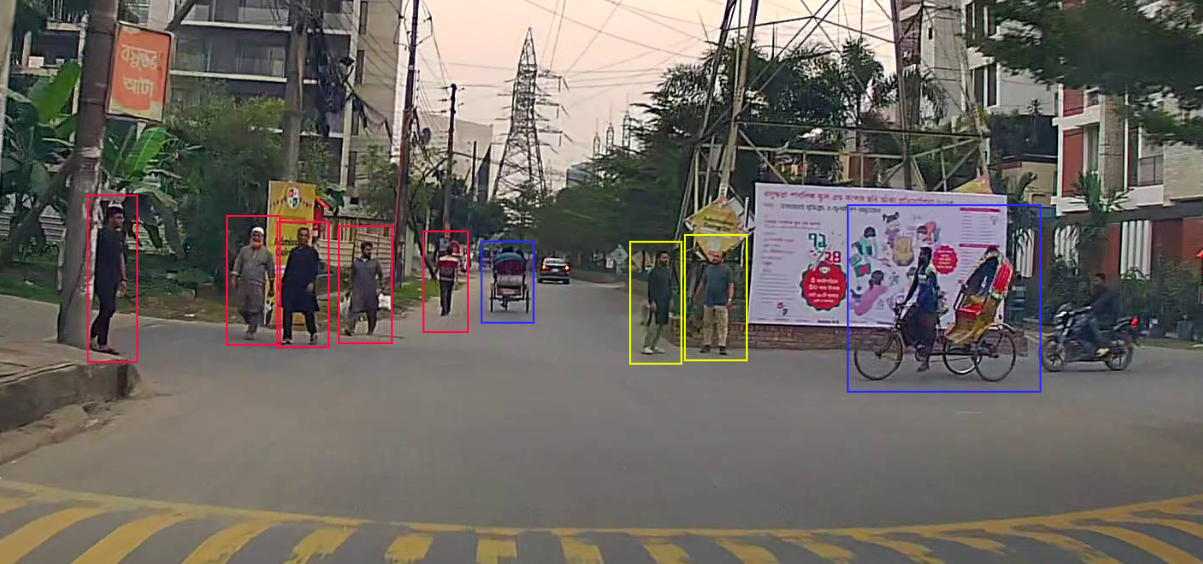
\includegraphics[width=1\textwidth]{images/bd.png} 
    % Uncomment the line above and change the filename to your actual image file
    \caption{Annotation sample from the BanglaTesla-PeD dataset using CVAT. Red Boxes: Pedestrian-Crosscing, Yollow Boxes:Pedestrian-NoCrosscing, and Blue Boxe: BanglaTeslas.}
    \label{fig:bd-ped}
\end{figure}
\end{itemize}
  
    
    \item \textbf{Multi-Level Annotation Schema:} CVAT (Computer Vision Annotation Tool) was utilized to incorporate a multi-level annotation schema which expands the IDD-PeD format to allow for region-specific behaviors:
    \begin{enumerate}
    
    
        \item \textbf{Spatial Annotations:} Pedestrians and ``BanglaTeslas'' were tightly bounding box annotated on a frame-by-frame basis. Following IDD-PeD, the occlusion levels (None, Partial, Full) were also indicated, so that the very high density of visual clutter present in Dhaka's traffic was quantified \cite{bokkasam2025pedestrian}.
        \item \textbf{Trajectory Tracking:} All agents were given Unique Track IDs that enabled the capturing of the temporal movement patterns over the 3--5 seconds sequences, making possible the analysis of long-term trajectory prediction.
        \item \textbf{Behavioral Characteristics:} The authors put forward region-specific behavioral labels that were not included in international datasets:
        \begin{itemize}
            \item ``Lane Splitting'': Marked for vehicles that are making aggressive maneuvers between the already established lanes.
            \item ``Rolling Gap Acceptance'': A situation that is very common in Dhaka where pedestrians come into the traffic flow without waiting for a clear gap \cite{vasudevan2020pedestrian}.
        \end{itemize}
        \item \textbf{Interaction Annotations:} These are binary indicators that signal the instances of ``Evasive Maneuvers'' where either the ego-vehicle or the ``BanglaTesla'' had to alter the route due to the unpredictability of the pedestrians' movements.
        \item \textbf{Scene Context:} These are the annotations that describe the unstructured road types, for instance, ``Unmarked Intersection,'' ``Midblock Jaywalking Zone,'' or ``Temporary Bus Stop.''
   \end{enumerate}
   
      \end{itemize}
   
    \begin{figure}[htbp]
    \centering
    % --- First Subfigure (Left) ---
    \begin{subfigure}[b]{0.48\textwidth}
        \centering
        % REPLACE 'images/bd.png' with your FIRST image file
        \includegraphics[height=6.5cm,width=1\linewidth]{images/t5.png}
        \caption{Scenario 1:No Trajection}
        \label{fig:bd_sample1}
    \end{subfigure}
    \hfill % Adds horizontal spacing between the two figures
    % --- Second Subfigure (Right) ---
    \begin{subfigure}[b]{0.48\textwidth}
        \centering
        % REPLACE 'images/bd.png' with your SECOND image file
        \includegraphics[height=6.5cm,width=1\linewidth]{images/t7.png}
        \caption{Scenario 2: Trajection}
        \label{fig:bd_sample2}
    \end{subfigure}

    % --- Main Figure Caption ---
    \caption{Annotated Bangla Tesla Trajectory Line}
    \label{fig:bd-tesla-trajectory}
\end{figure}


The dataset reflects very active interactions taking place in situations where the ego-vehicle's speed is varying constantly in the range of 0--40 km/h. A considerable part of the data is related to non-signalized intersections as these are the spots that mostly contribute to the overall conflict points in Dhaka's surroundings \cite{baig2024badodd}.



%\subsubsection{Comparative Data Statistics Analysis}
%
%\begin{itemize}
%
%\item \textbf{Dataset scale and annotation density:}  
%IDD-PeD has the larger absolute size, for which the number of unique pedestrian images, number of bounding box annotations, and number of annotated frames are 5K, 686K, and 205K, respectively. In the case of Banglatesla-PeD, these numbers are 3.2K, 440K, and 145K, respectively.These amounts translate to a pedestrian, bounding box, and frame reduction of 36\% and 29\%, respectively. However, the number of behavior classes for the two benchmark datasets remains the same, at 19. With respect to annotation factors, the two benchmark datasets also share similarities along the lines of interaction, occlusion, group behavior, location, nighttime appearance, and the presence of signaled intersections. Consequently, annotation density per pedestrian and per frame for the Banglatesla-PeD benchmark dataset remains relatively high, despite the reduction in the scale of the benchmarking.
%
%
%\begin{figure}[H]
%    \centering
%    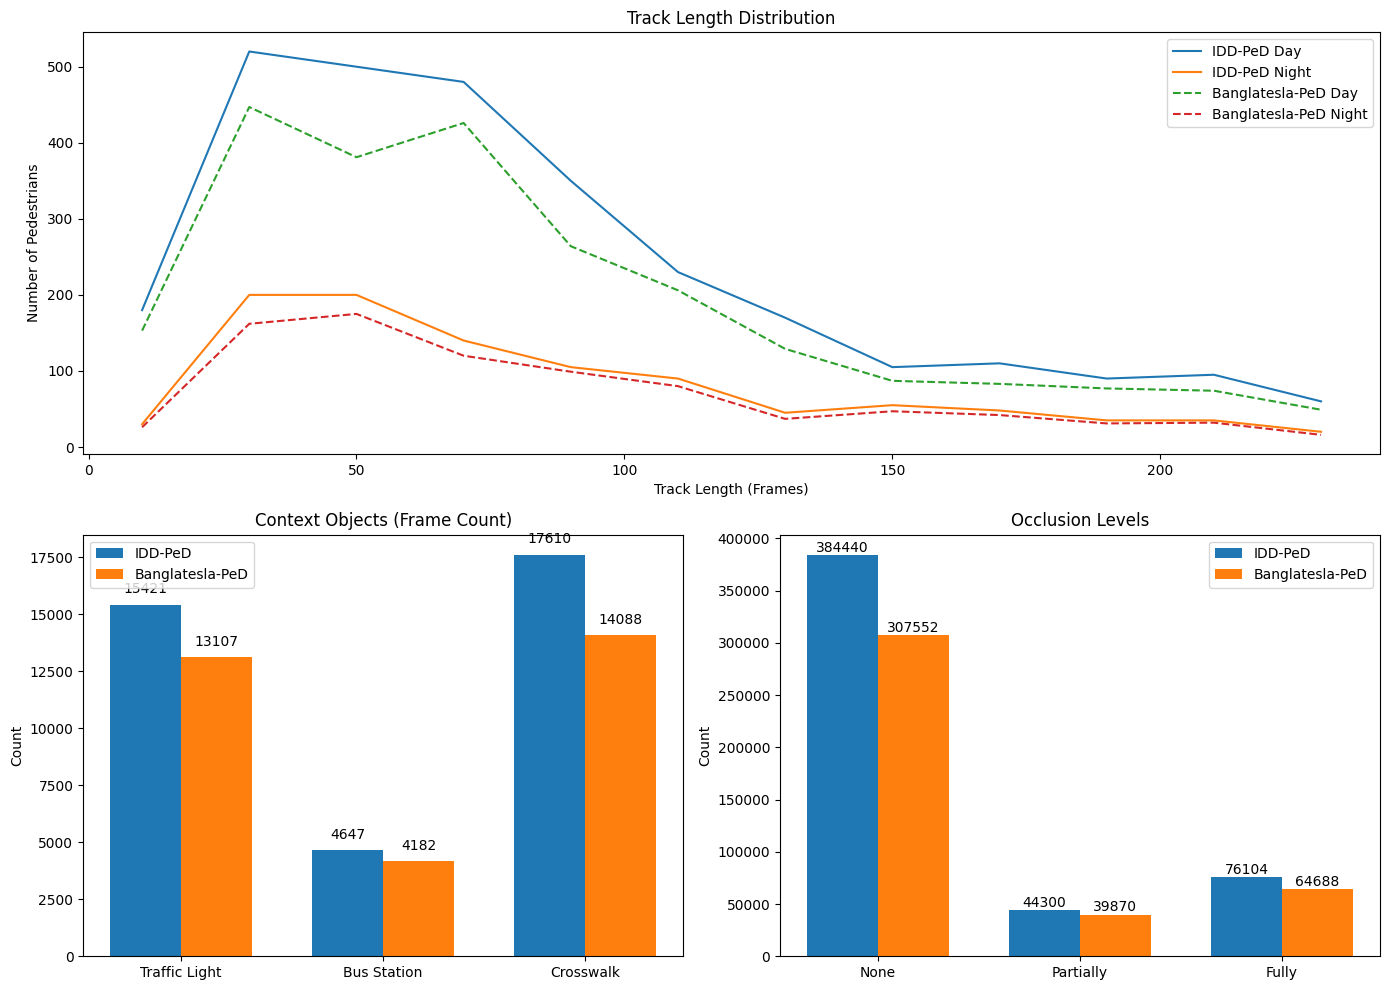
\includegraphics[width=\linewidth]{images/12.png}
%    \caption{Comparison of environment-level impact on pedestrian behavior prediction across IDD-PeD and Banglatesla-PeD under illumination, interaction, occlusion, and signalization conditions.}
%    \label{fig:env_comparison}
%\end{figure}
%
%\item \textbf{Environment-level statistics and performance sensitivity:}  
%When considering illumination variation, the AUC of IDD-PeD is about 0.51 during the day and 0.52 during night hours. It shows a relative variation of about 2-3\%. It clearly shows a moderate variation in the AUC with respect to illumination variation. The effect of interaction in IDD-PeD shows a fall in the performance AUC from 0.50 in non-interaction images to 0.49 in high interaction images. The effect is relatively negligible as it shows a mere fall of about 2\%. The effect of occlusion and signalization shows relatively less effect as the AUC variation remains within 0.5\% in both cases. Banglatesla-PeD follows the same trends as IDD-PeD but shows relatively less deviation among the samples based on the environmental parameters.
%
%\item \textbf{Trajectory length distribution:}  
%From the trajectory stats, it can be observed that IDD-PeD has many long pedestrian trajectories. During the day, the maximum density of trajectories falls in the range of 30-70 frames, with the count close to 500, and even up to 150-210 frames, the density maintains between 90 and 110 trajectories. At night, the trajectories are less dense, peaking at about 200 trajectories for the 30-50 frame range and dropping to less than 50 for the frames beyond 150. Banglatesla-PeD has a more compact density of short to medium trajectories, especially between the frames of 20 and 100, and relatively less density of long trajectories. These are mostly interruptions by congestion, occlusion, and interactions, which are usually found in heavily populated areas.
%
%\item \textbf{Contextual object statistics:}  
%In IDD-PeD, the frames having traffic signals, crosswalks, and bus stops are of about 15,421, 17,610, and 4,647, respectively. The listing of crosswalks and traffic signals within the total context/object labels recognizes the importance of structured/semi-structured pedestrian crossing scenarios. The categories of the context are preserved by Banglatesla-PeD, though with fewer absolute numbers, as well as the elevated representation of crosswalks and mixed context images. It means the significance of informal and poorly regulated pedestrian activities of crossing the road.
%
%\item \textbf{Characteristics of occlusion:}  
%The number of occlusion statistics in IDD-PeD is mostly attributed to the fully visible pedestrians, with about 384,440 non-occluded instances; this is followed by 44,300 partially occluded and 76,104 fully occluded instances. The above data accounts for about 76\% non-occluded, 9\% partial occlusions, and 15\% full occurrences of the pedestrians. The Banglatesla-PeD dataset, which has a relatively lower absolute number of images, has a greater percentage of partial and full occurrences of the pedestrians.
%
%
%\begin{figure}[H]
%    \centering
%    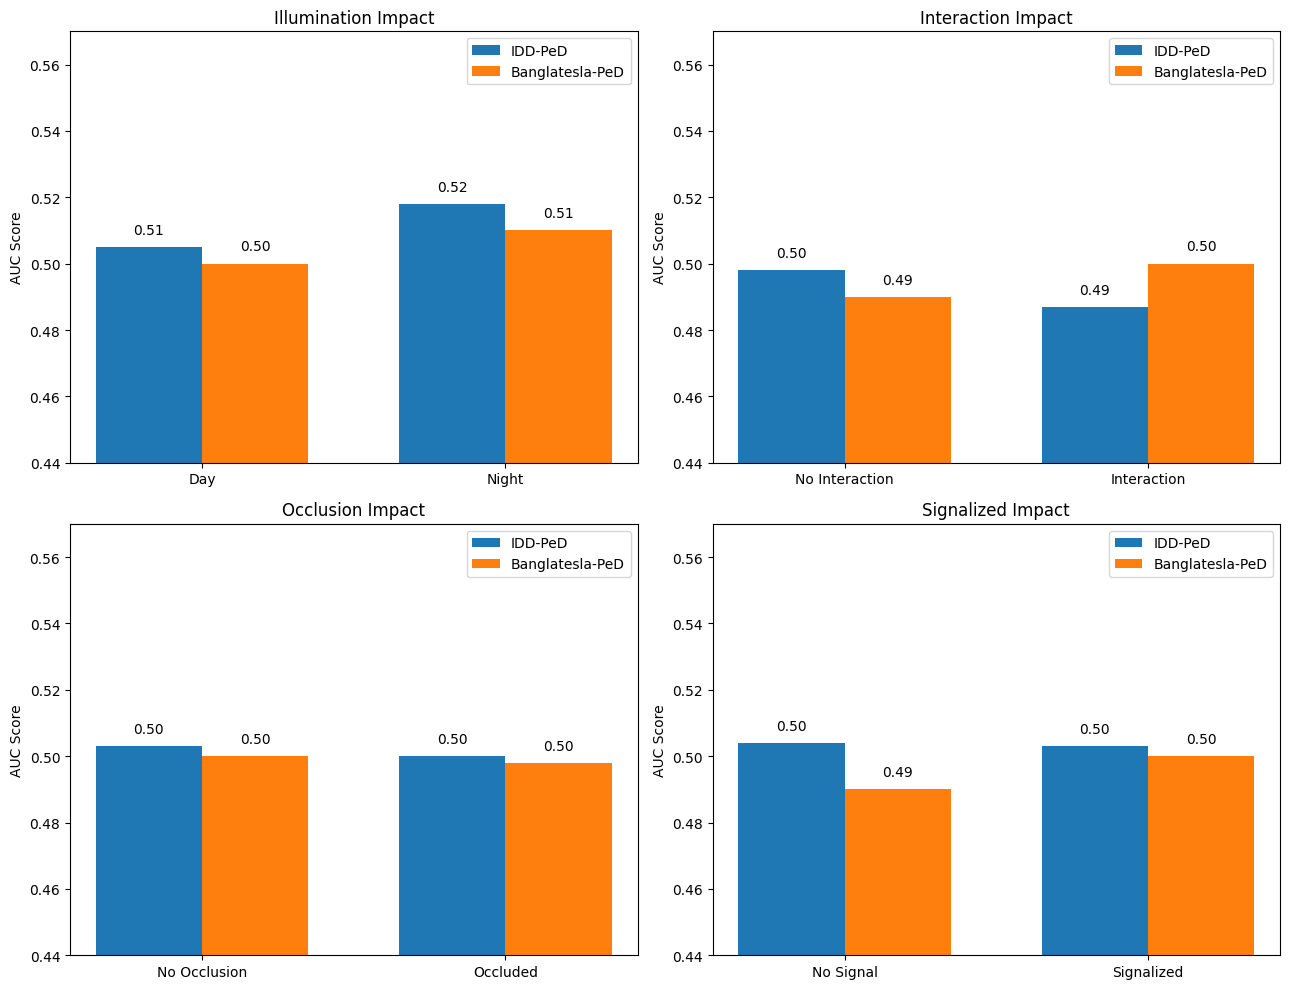
\includegraphics[width=\linewidth]{images/11.png}
%    \caption{Comparison of trajectory length distribution, contextual object frequency, and occlusion statistics between IDD-PeD and Banglatesla-PeD.}
%    \label{fig:stats_comparison}
%\end{figure}
%
%\item \textbf{Distribution of attributes and behaviors:}  
%The attribute-level statistics available in IDD-PeD show a remarkable imbalance between classes. The routine behaviors like walking and standing are quite common, with around 283,717 frames of the former and over 300K frames associated with standing, against 44,044 frames related to distracted pedestrians and 17,979 frames associated with agent interaction. The behaviors associated with crossings are quite imbalanced, with 101,155 frames depicting jaywalking and 27,074 depicting regular crossing, against just 502 frames showing fast crossing. The demographic attributes are quite sparse, with just 360 frames related to child, 312 to teenager, 8,649 to adult, and 512 frames classified as senior. Bangletesla-PeD shows a flatter curve related to these attributes, with relatively stronger appearance of interaction-related and rare classes, compensating for the overall sparseness despite fewer annotations.
%
%\begin{figure}[H]
%    \centering
%    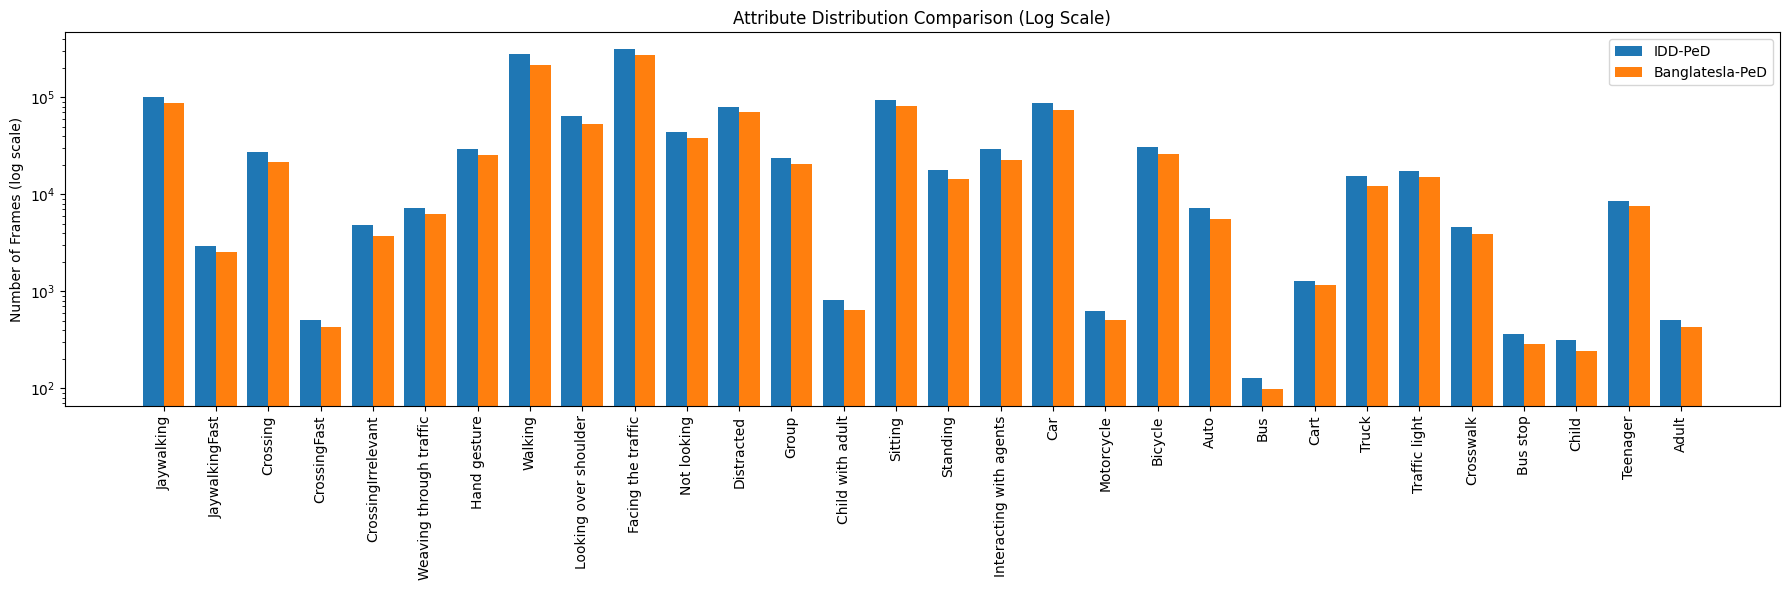
\includegraphics[width=\linewidth]{images/13.png}
%    \caption{Attribute distribution comparison (log scale) between IDD-PeD and Banglatesla-PeD across pedestrian behaviors, interactions, traffic entities, and demographic categories.}
%    \label{fig:attribute_comparison}
%\end{figure}
%
%\item \textbf{Complete statistical comparison:}  
%In numerical terms, IDD-PeD offers larger-scale data, longer uninterrupted trajectory data, as well as a greater number of fully visible pedestrians. Banglatesla-PeD, being about two-thirds smaller than IDD-PeD in frames as well as bounding boxes, provides greater contextual density, greater occlusion ratios, as well as more balanced distribution of attributes. These disparities in statistics, therefore, show that Banglatesla-PeD covers complementary aspects of IDD-PeD, focusing more on scenarios of dense interaction as well as complex urban traffic contexts.
%\end{itemize}

\subsubsection{Comparative Data Statistics Analysis}

\begin{itemize}

\item \textbf{Dataset scale and annotation density:}  
IDD-PeD has the larger absolute size, for which the number of unique pedestrian images, number of bounding box annotations, and number of annotated frames are 5K, 686K, and 205K, respectively. In the case of Banglatesla-PeD, these numbers are 3.2K, 440K, and 145K, respectively. These amounts translate to a pedestrian, bounding box, and frame reduction of 36\% and 29\%, respectively. However, the number of behavior classes for the two benchmark datasets remains the same, at 19. With respect to annotation factors, the two benchmark datasets also share similarities along the lines of interaction, occlusion, group behavior, location, nighttime appearance, and the presence of signaled intersections. Consequently, annotation density per pedestrian and per frame for the Banglatesla-PeD benchmark dataset remains relatively high, despite the reduction in the scale of the benchmarking.

% Changed [H] to [htbp] to allow text to share the page
\begin{figure}[htbp]
    \centering
    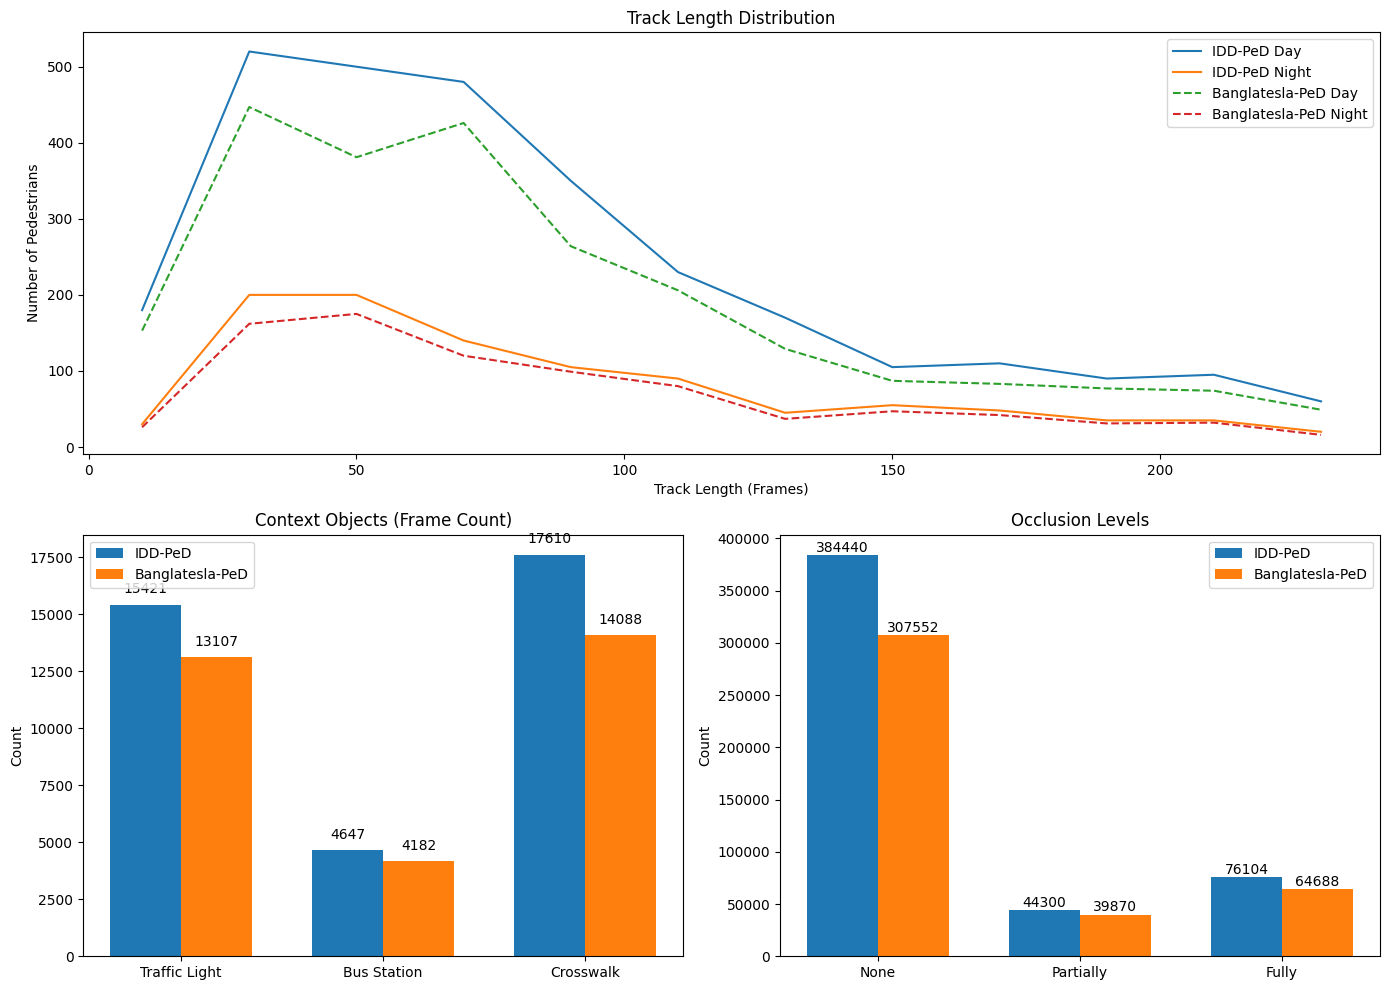
\includegraphics[width=\linewidth]{images/12.png}
    \caption{Comparison of environment-level impact on pedestrian behavior prediction across IDD-PeD and Banglatesla-PeD under illumination, interaction, occlusion, and signalization conditions.}
    \label{fig:env_comparison}
\end{figure}

\item \textbf{Environment-level statistics and performance sensitivity:}  
When considering illumination variation, the AUC of IDD-PeD is about 0.51 during the day and 0.52 during night hours. It shows a relative variation of about 2-3\%. It clearly shows a moderate variation in the AUC with respect to illumination variation. The effect of interaction in IDD-PeD shows a fall in the performance AUC from 0.50 in non-interaction images to 0.49 in high interaction images. The effect is relatively negligible as it shows a mere fall of about 2\%. The effect of occlusion and signalization shows relatively less effect as the AUC variation remains within 0.5\% in both cases. Banglatesla-PeD follows the same trends as IDD-PeD but shows relatively less deviation among the samples based on the environmental parameters.

\item \textbf{Trajectory length distribution:}  
From the trajectory stats, it can be observed that IDD-PeD has many long pedestrian trajectories. During the day, the maximum density of trajectories falls in the range of 30-70 frames, with the count close to 500, and even up to 150-210 frames, the density maintains between 90 and 110 trajectories. At night, the trajectories are less dense, peaking at about 200 trajectories for the 30-50 frame range and dropping to less than 50 for the frames beyond 150. Banglatesla-PeD has a more compact density of short to medium trajectories, especially between the frames of 20 and 100, and relatively less density of long trajectories. These are mostly interruptions by congestion, occlusion, and interactions, which are usually found in heavily populated areas.

\item \textbf{Contextual object statistics:}  
In IDD-PeD, the frames having traffic signals, crosswalks, and bus stops are of about 15,421, 17,610, and 4,647, respectively. The listing of crosswalks and traffic signals within the total context/object labels recognizes the importance of structured/semi-structured pedestrian crossing scenarios. The categories of the context are preserved by Banglatesla-PeD, though with fewer absolute numbers, as well as the elevated representation of crosswalks and mixed context images. It means the significance of informal and poorly regulated pedestrian activities of crossing the road.

\item \textbf{Characteristics of occlusion:}  
The number of occlusion statistics in IDD-PeD is mostly attributed to the fully visible pedestrians, with about 384,440 non-occluded instances; this is followed by 44,300 partially occluded and 76,104 fully occluded instances. The above data accounts for about 76\% non-occluded, 9\% partial occlusions, and 15\% full occurrences of the pedestrians. The Banglatesla-PeD dataset, which has a relatively lower absolute number of images, has a greater percentage of partial and full occurrences of the pedestrians.

% Changed [H] to [htbp]
\begin{figure}[htbp]
    \centering
    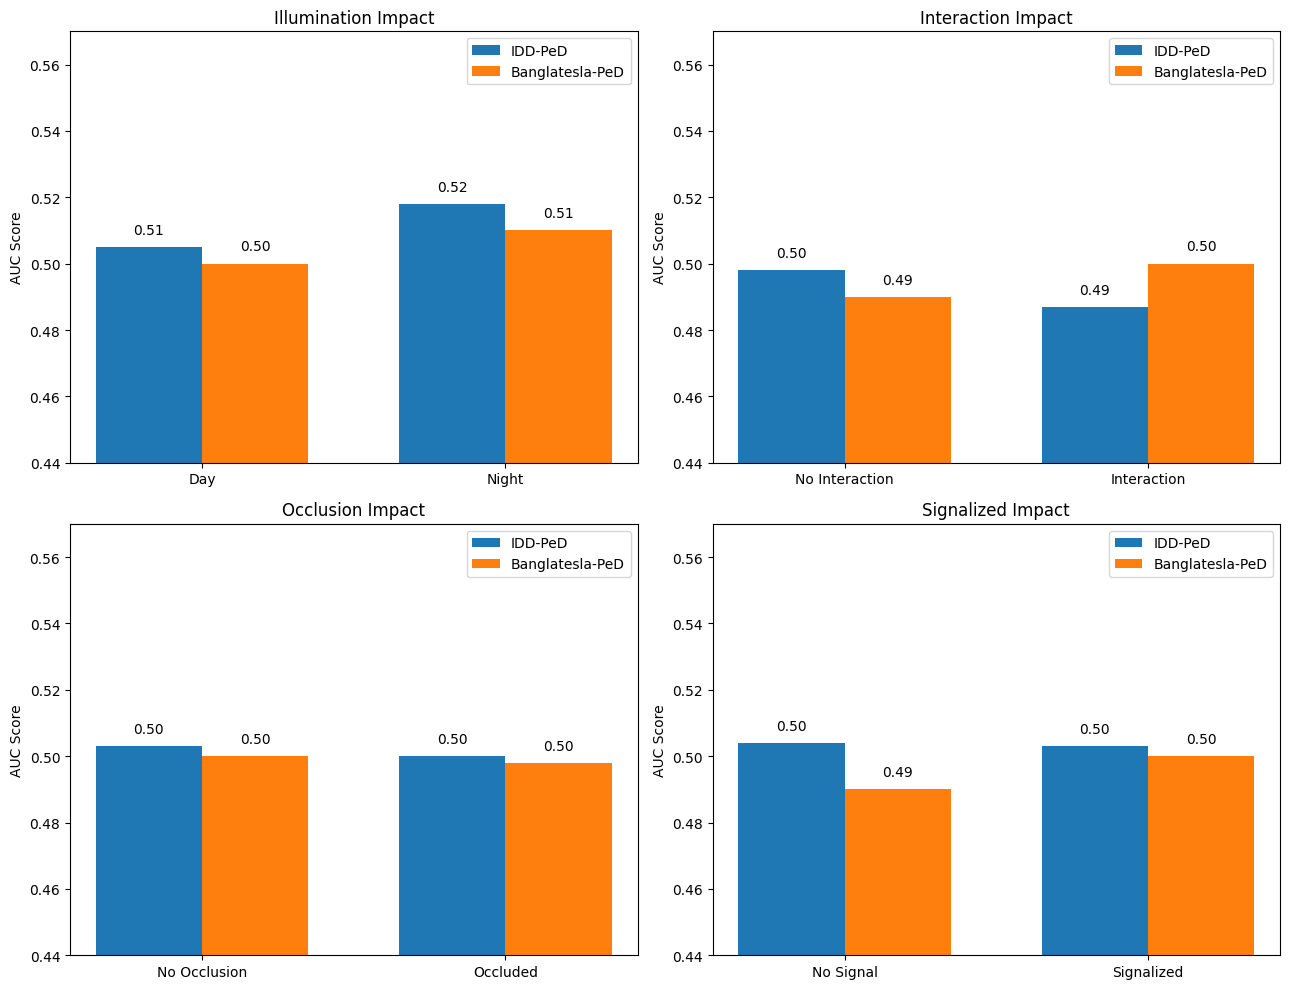
\includegraphics[width=\linewidth]{images/11.png}
    \caption{Comparison of trajectory length distribution, contextual object frequency, and occlusion statistics between IDD-PeD and Banglatesla-PeD.}
    \label{fig:stats_comparison}
\end{figure}

\item \textbf{Distribution of attributes and behaviors:}  
The attribute-level statistics available in IDD-PeD show a remarkable imbalance between classes. The routine behaviors like walking and standing are quite common, with around 283,717 frames of the former and over 300K frames associated with standing, against 44,044 frames related to distracted pedestrians and 17,979 frames associated with agent interaction. The behaviors associated with crossings are quite imbalanced, with 101,155 frames depicting jaywalking and 27,074 depicting regular crossing, against just 502 frames showing fast crossing. The demographic attributes are quite sparse, with just 360 frames related to child, 312 to teenager, 8,649 to adult, and 512 frames classified as senior. The curve of Bangletesla-PeD concerning these attributes is flatter, and the interaction-related and rare classes appear relatively strongly, which is compensating the overall sparseness despite the low number of annotations.

% Changed [H] to [htbp]
\begin{figure}[htbp]
    \centering
    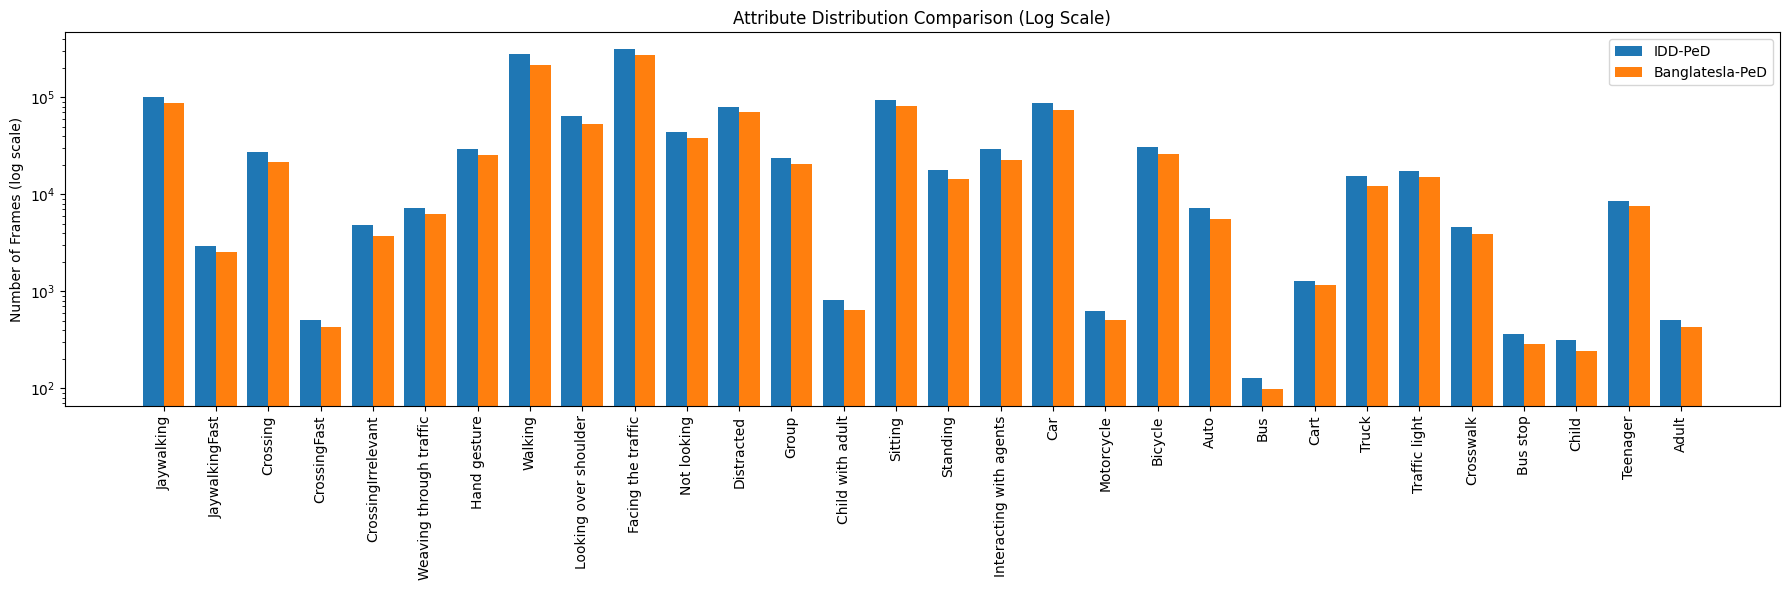
\includegraphics[width=\linewidth]{images/13.png}
    \caption{Attribute distribution comparison (log scale) between IDD-PeD and Banglatesla-PeD across pedestrian behaviors, interactions, traffic entities, and demographic categories.}
    \label{fig:attribute_comparison}
\end{figure}

\item \textbf{Complete statistical comparison:}  
In numerical terms, IDD-PeD offers larger-scale data, longer uninterrupted trajectory data, as well as a greater number of fully visible pedestrians. Banglatesla-PeD, being about two-thirds smaller than IDD-PeD in frames as well as bounding boxes, provides greater contextual density, greater occlusion ratios, as well as more balanced distribution of attributes. These disparities in statistics, therefore, show that Banglatesla-PeD covers complementary aspects of IDD-PeD, focusing more on scenarios of dense interaction as well as complex urban traffic contexts.
\end{itemize}
\clearpage
\section{Implementation and Results}

\subsection{System Model Architecture Design}

The architecture of the model is envisioned as a modular pipeline. It takes unprocessed egocentric videos as the input and generates the trajectory probability for various traffic entities as the output. The pipeline integrates three sequential modules: Perception \& State Estimation, Feature Encoding, and Multimodal Prediction \cite{bokkasam2025pedestrian}.

%\begin{figure}[H]
%    \centering
%    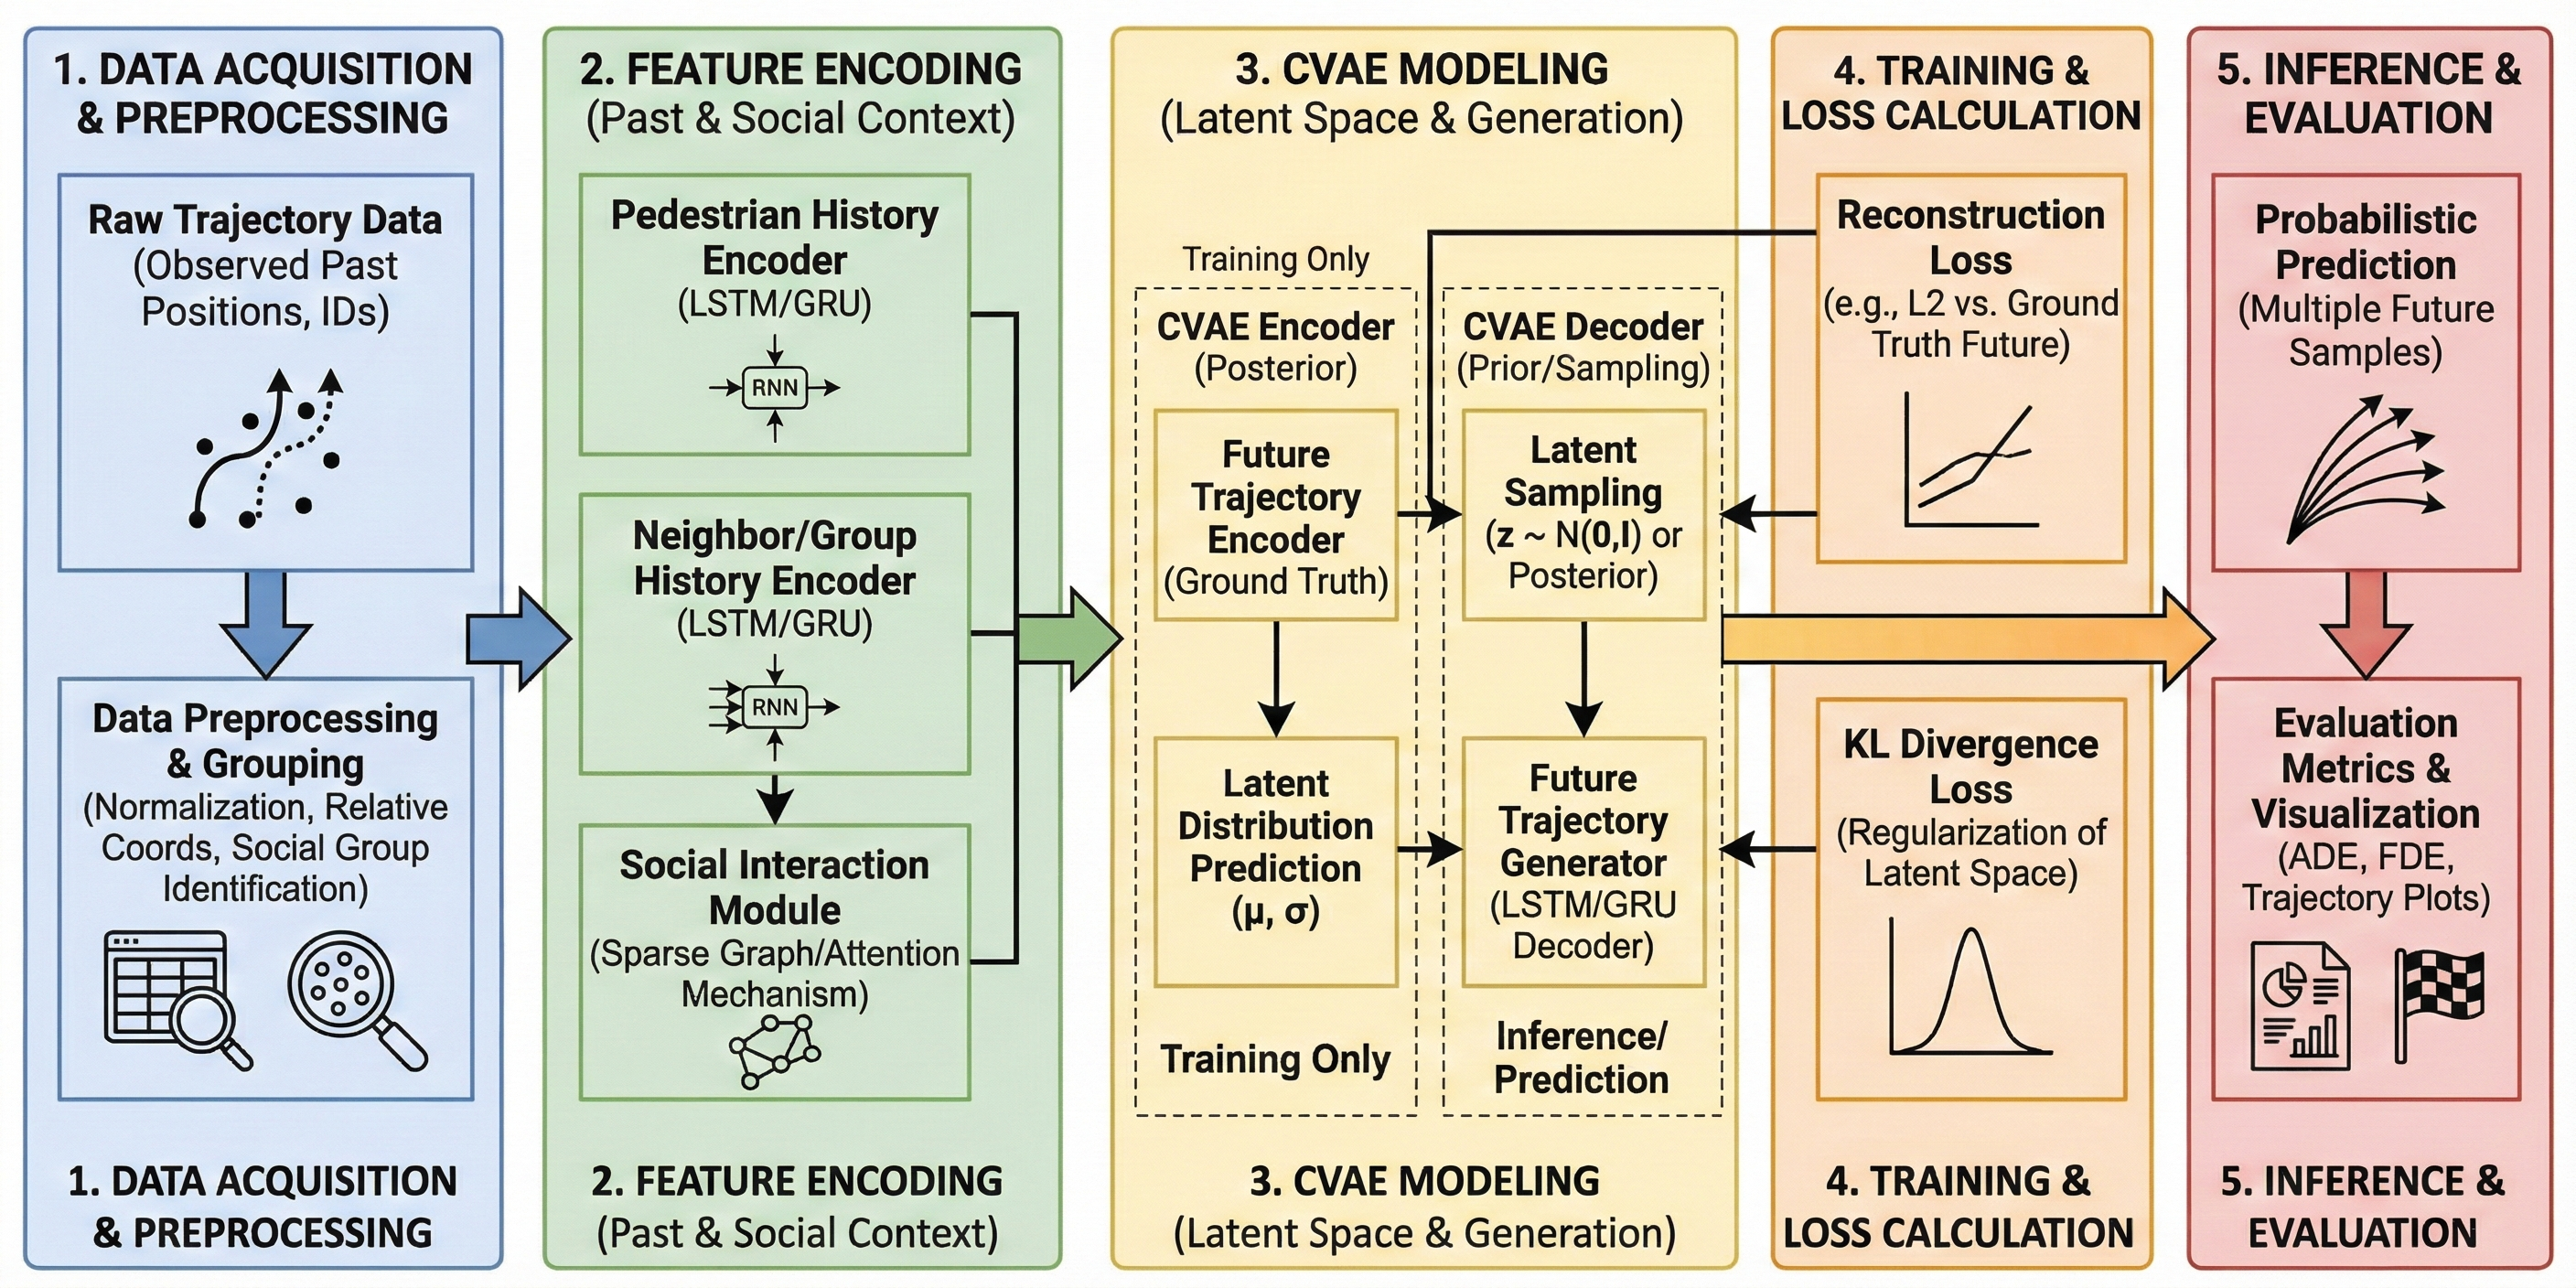
\includegraphics[width=\linewidth]{images/SGNetPTP.png}
%    \caption{Syetem Trajectory Model Architecture: SGNet}
%    \label{fig:SGNet-PIP}
%\end{figure}

\begin{figure}[htbp]
    \centering
    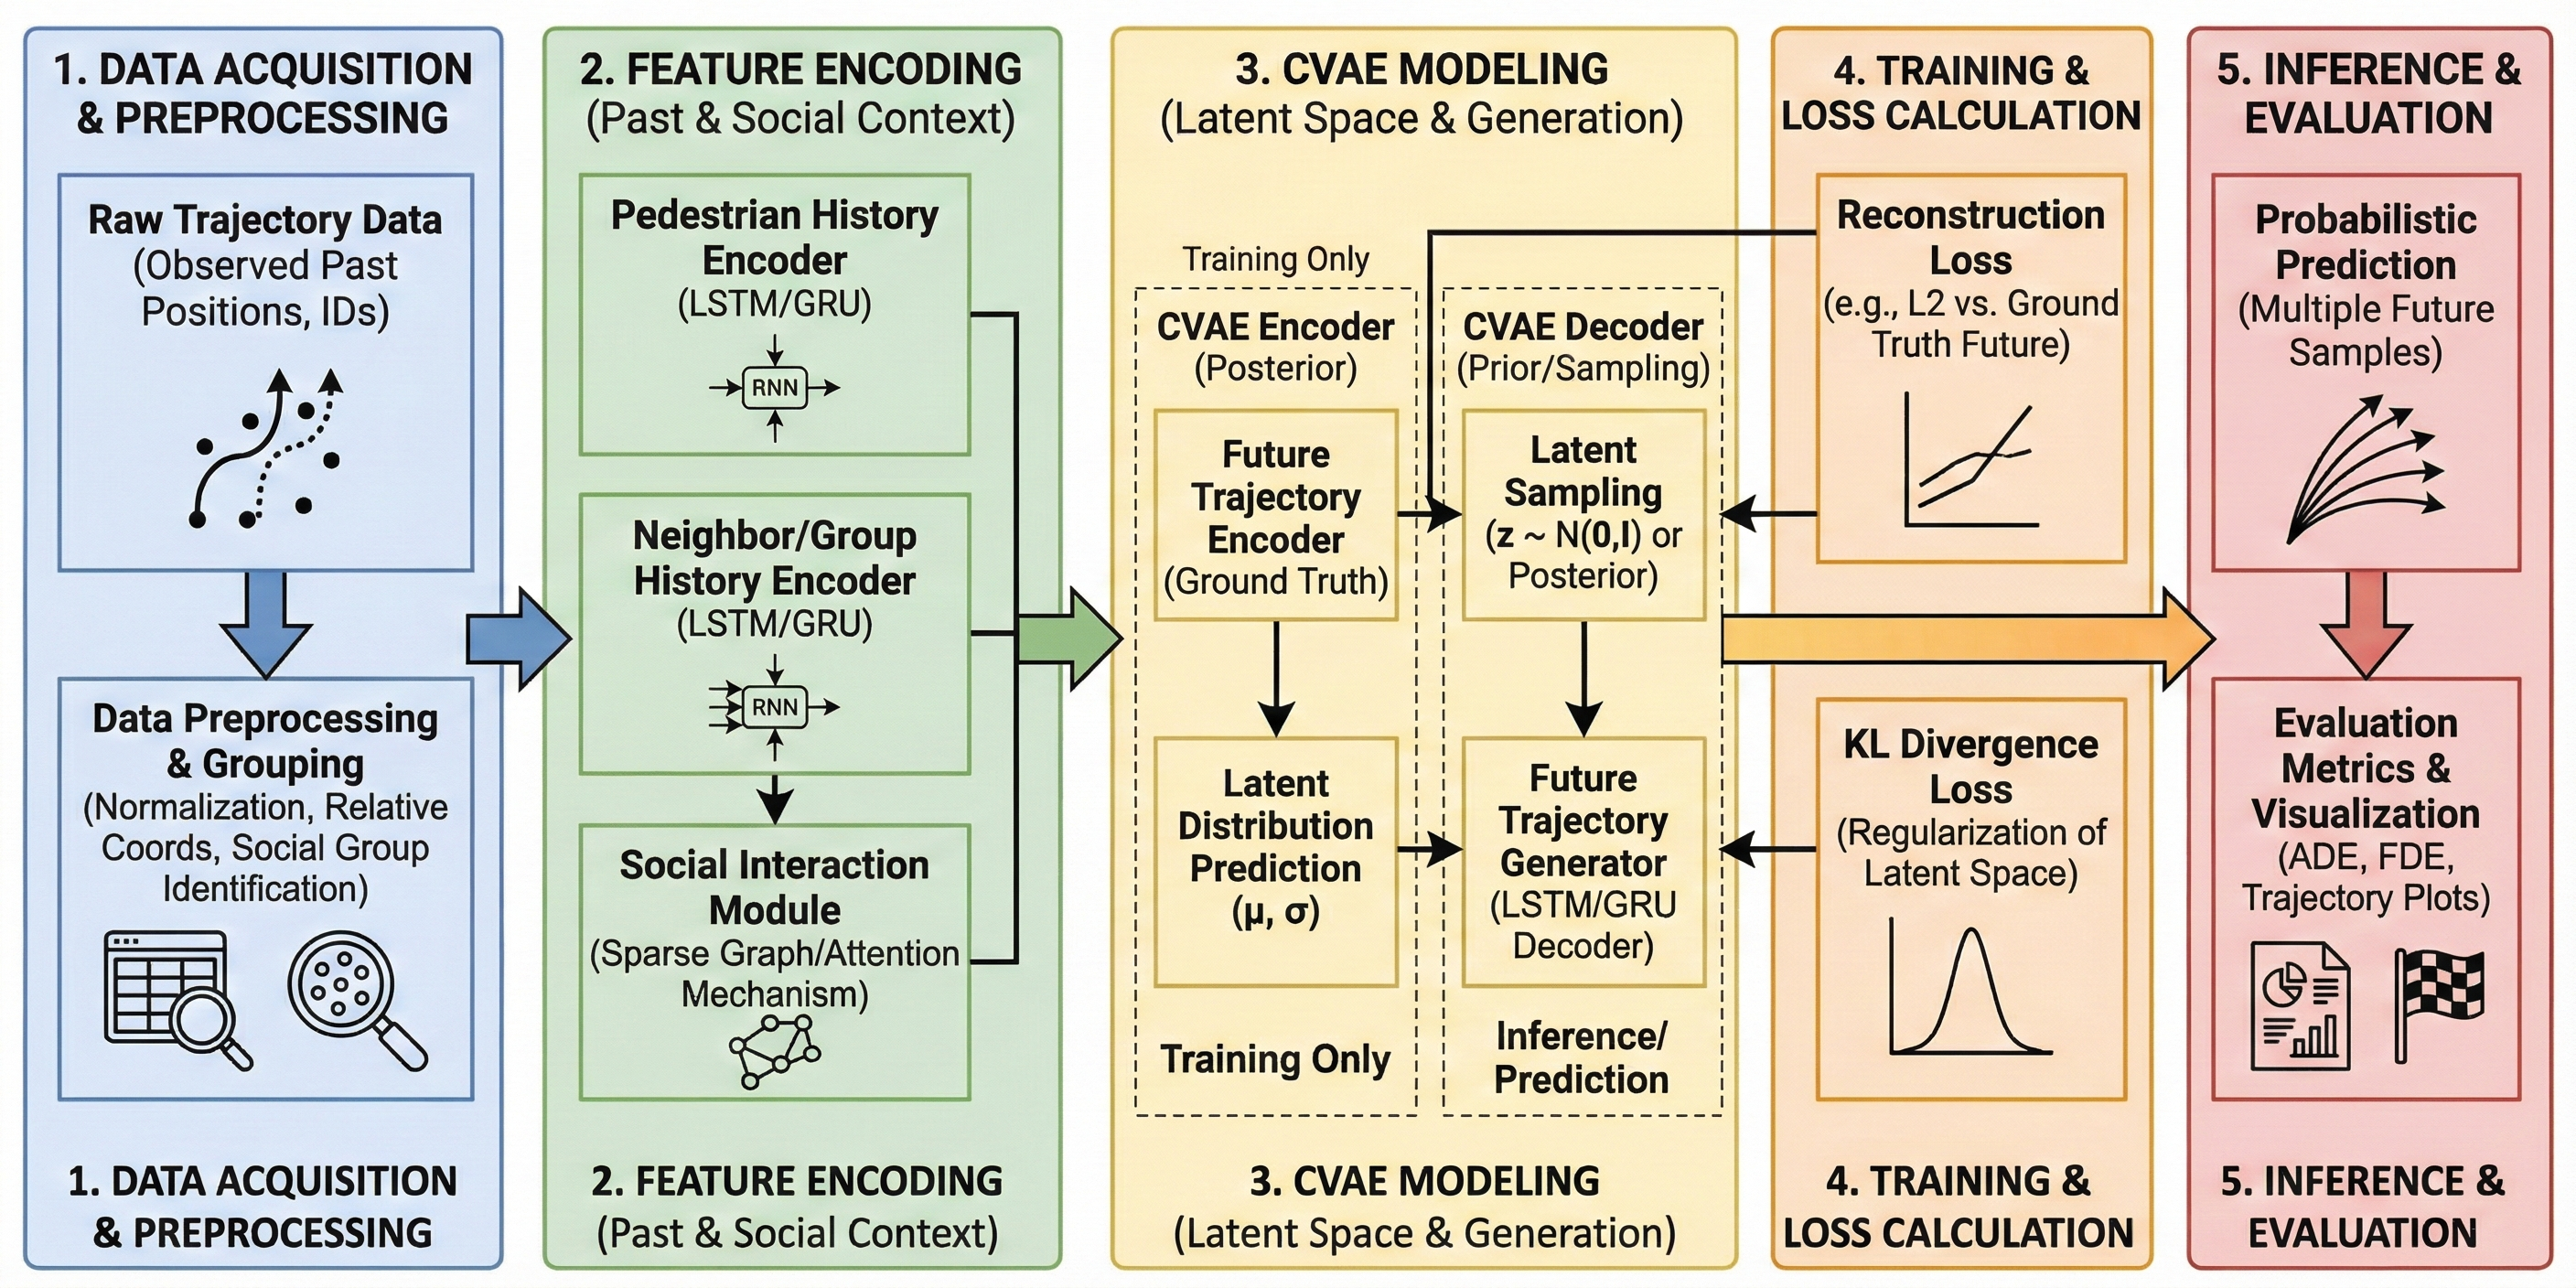
\includegraphics[width=\linewidth]{images/SGNetPTP.png}
    \caption{System Trajectory Model Architecture: SGNet}
    \label{fig:SGNet-PIP}
\end{figure}

\subsubsection{Perception \& State Estimation Module}
The raw video frames are denoted as $I_t$. These are initially processed to yield the observed states of all agents.

\paragraph{Detection and Tracking:} A pre-trained detector detects agents classified as Pedestrians, ``BanglaTeslas'' \cite{jagonews2025banglatesla}, and Vehicles. The $i^{th}$ tracked agent receives a track $T_i$. Bounding box coordinates, $B_t = (x_t, y_t, w_t, h_t)$ over an observation window of length $t_{obs} = 8$ frames (about 0.5 seconds).

\paragraph{Compensation of ego-motion:} To address the ego-motion of the ego-vehicle, which is especially significant in the unstructured traffic conditions of Dhaka \cite{baig2024badodd}, the motion of all tracked agents needs to be referred to a unified egocentric coordinate frame defined by the geometric center of the camera frame.

\subsubsection{Trajectory Prediction Architecture (Stochastic Engine)}
The Stochastic Goal-Driven Network (SGNet) \cite{wang2022stepwise} architecture is used for the dominant trajectory prediction problem and is also adapted to account for the bi-modal acceleration patterns of the ``BanglaTeslas'' \cite{jagonews2025banglatesla}.


\begin{figure}[htbp]
    \centering
    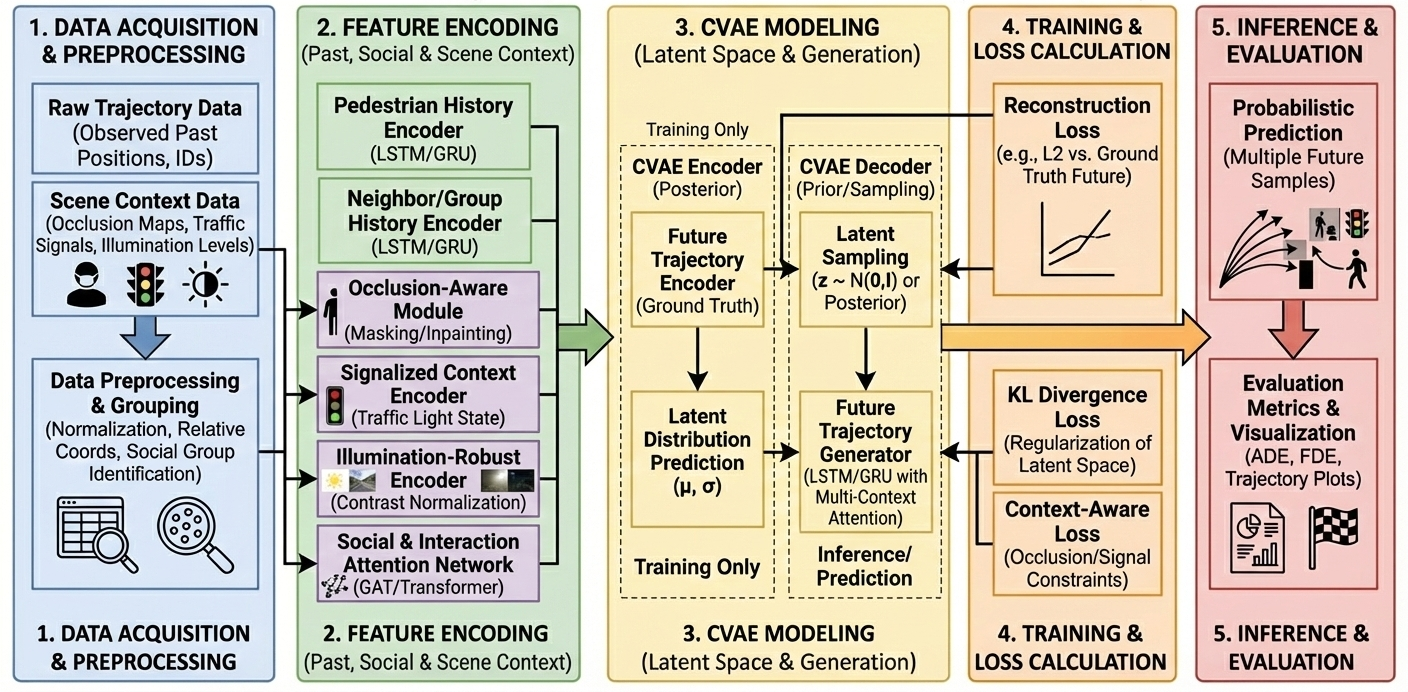
\includegraphics[width=\linewidth]{images/SGNet4.png}
    \caption{System Trajectory Model Architecture (Occlusion, Signalized, Illumination, Interaction): SGNet}
    \label{fig: SGNet-PTP}
\end{figure}


\paragraph{Input Representation:} The model accepts the observed trajectory pair $X_{obs} = \{(x_t, y_t) \mid t = 1 \dots t_{obs}\}$.

\paragraph{CVAE Mechanism:} Unlike traditional models, such as PIETraj \cite{rasouli2019pie}, which attach the input to the predicted trajectory, this variant utilizes the Conditional Variational Autoencoder (CVAE). It encodes the observed trajectory pair $X_{obs}$ and the ground truth trajectory $Y_{GT}$ into the joint latent space $Z \sim N(\mu, \sigma)$.


\begin{figure}[htbp]
    \centering
    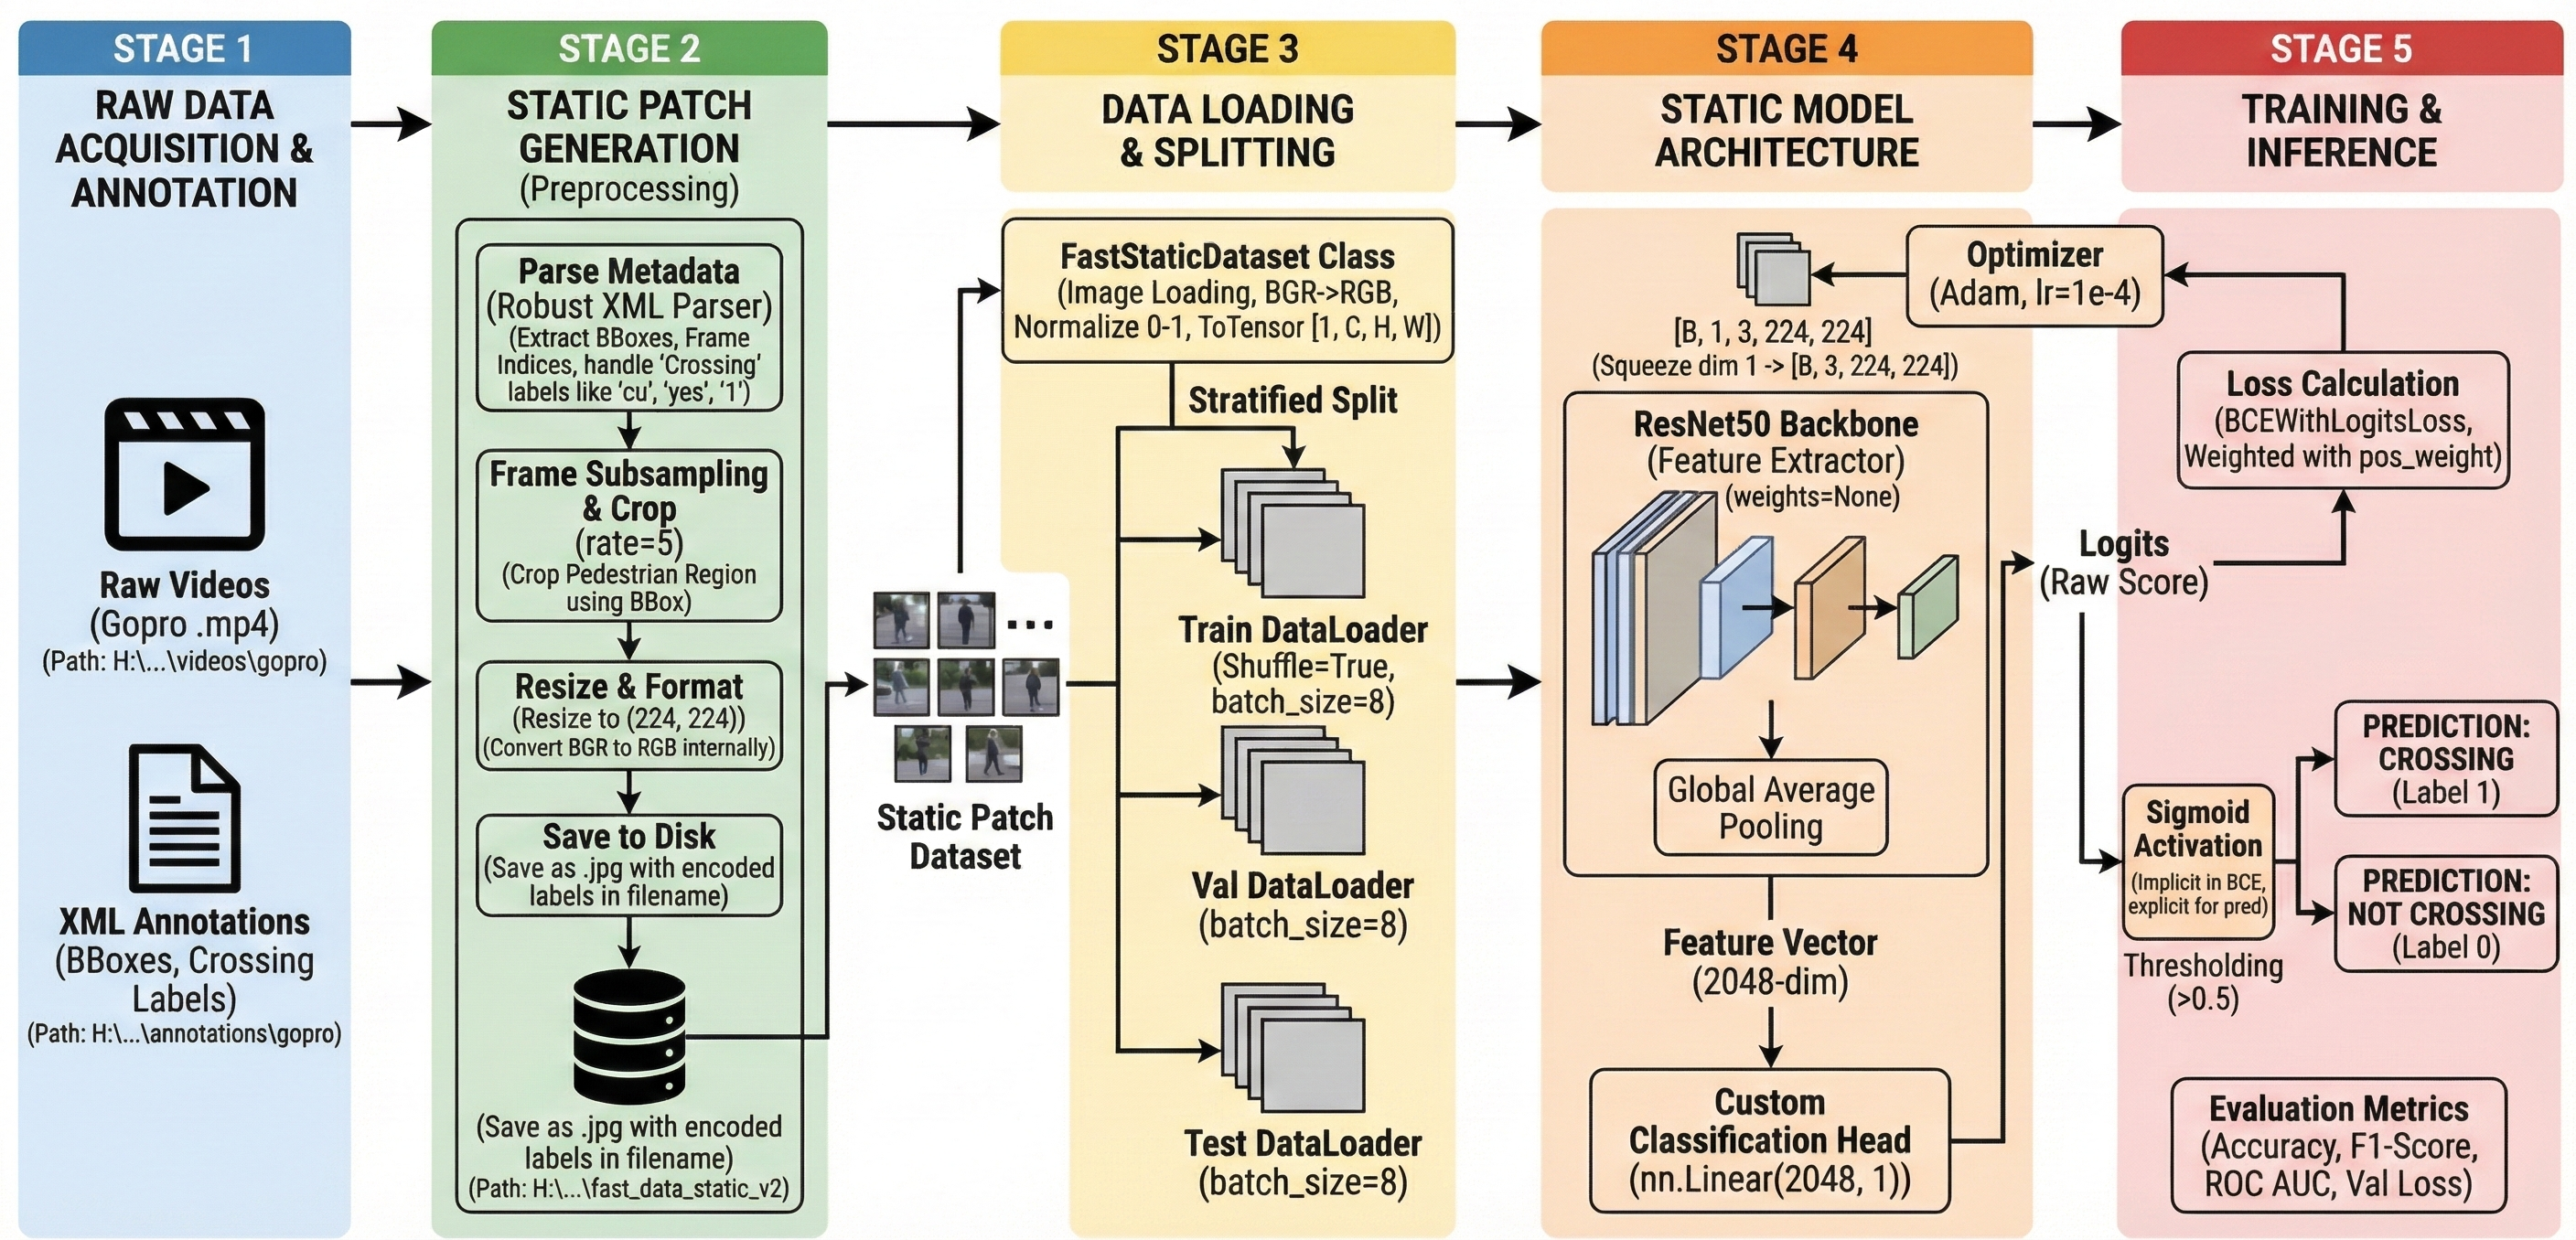
\includegraphics[width=\linewidth]{images/StaticPIP.png}
    \caption{System Prediction Model Architecture: Static (ResNet50)}
    \label{fig:attribute_comparison}
\end{figure}

\paragraph{Bi-modal goal estimation:} It gets $K = 20$ potential trajectories from the joint space. This helps the model predict both ``yield'' (stop) and ``merge'' (accelerate) actions meant for the individual BanglaTesla. This is based on the model’s capability to capture the inherent uncertainty of the environment.

\subsubsection{Intention Prediction Architecture (PIP)}
In addition to path trajectory formation, another aspect that is determined by the ``Intention Prediction'' module is the possibility of crossing pedestrians present on the roads.


\begin{figure}[htbp]
    \centering
    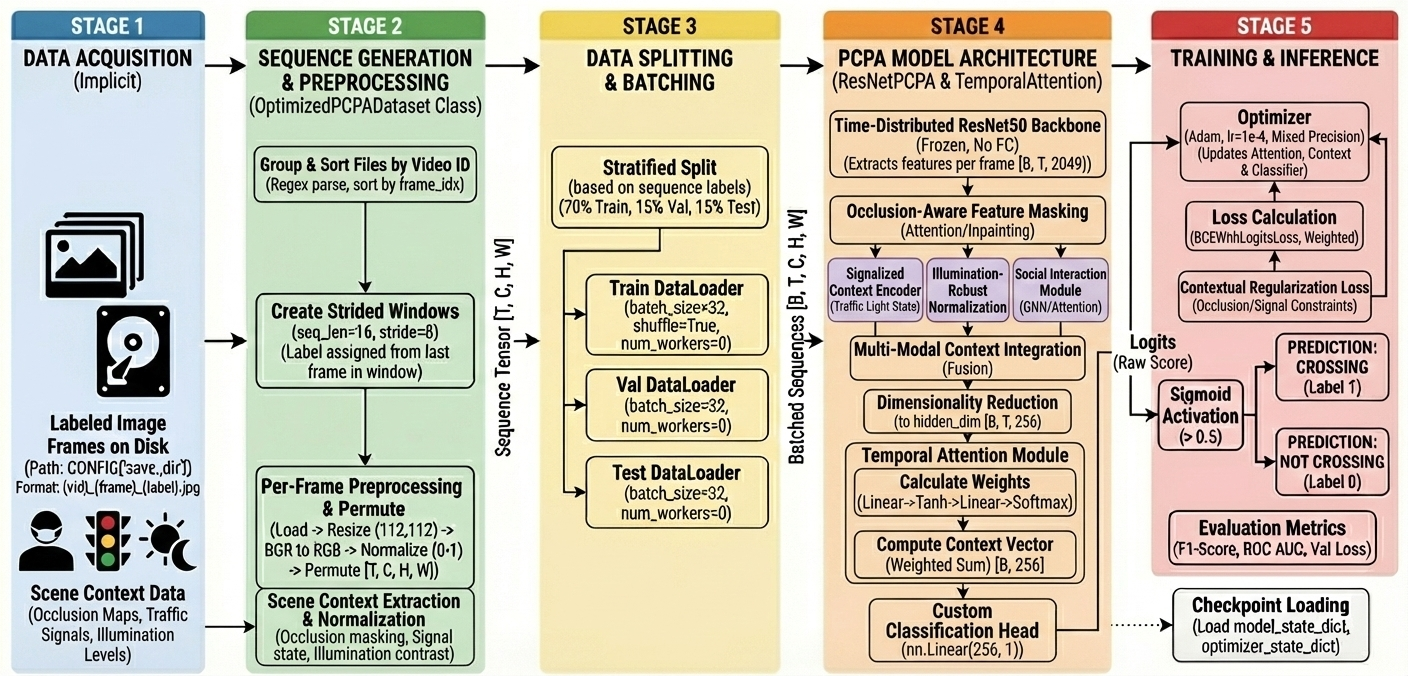
\includegraphics[width=\linewidth]{images/PCPA-4.png}
    \caption{ystem Trajectory Model Architecture (Occlusion, Signalized, Illumination, Interaction): PCPA}
    \label{fig:attribute_comparison}
\end{figure}

\paragraph{Specio-Temporal Fusion:} Pedestrian Crossing Prediction with Attention (PCPA) \cite{rasouli2019pie} can be considered as the model used for spatiotemporal fusion. Local box features (backbone CNN) and direct motion information (optical flow) are fused in the process of spatiotemporal processing.

\paragraph{Attention Mechanism:} The temporal attention module reduces the noise caused in unordered wait zones. This is achieved through the emphasis of the final 0.5 seconds before the rolling movements.

\subsection{Experimental Implementation Details}
To make our results on both IDD-PeD and the newly created ``BanglaTesla'' datasets reproducible, we applied a common training scheme on all architectures considered as baselines.

\subsubsection{Training Setup}

All experiments have been performed using the PyTorch deep learning toolkit on an available work-station with an NVIDIA GeForce RTX 3060 graphics card (12GB VRAM). Also, the computations were accelerated using CUDA 11.3 and CuDNN 8.2 for managing the computation burden due to spatiotemporal processing.

\paragraph{Hyperparameters:}  In Trajectory Prediction (PTP) models SGNet \cite{wang2022stepwise}, BiTraP \cite{yao2021bitrap} and PIETraj \cite{rasouli2019pie}, Adam was applied with an initial learning rate of $1e^{-3}$ and a weight decay of $1e^{-4}$. The size of the batch was set to 32 and this balanced the VRAM memory. Training epochs were capped at 100, incorporating an early stopping criterion where training ceased when the validation loss had not improved for 15 consecutive epochs for each model. In the Intention Prediction (PIP) model, the learning rate was reduced to $5e^{-4}$, incorporating the use of a weighted binary cross-entropy loss function, which dealt with the class imbalance issue of crossing/nocrossing classes.

\subsection{Experimental Results}
In this section, we will explain an overall assessment of the performance of our implementation in relation to what has been defined within current literature. Specifically, we will analyze results on the source domain ``IDD-PeD'' to validate our implementation, followed by the domain gap on our target ``BanglaTesla'' data set.

\subsubsection{Intention Prediction (PIP) Evaluation on IDD-PeD}
Our first benchmark was with respect to Pedestrian Intention Prediction model implementations on the IDD-PeD dataset. Table \ref{tab:pip_idd} compares our results with those from the papers (``Papers'') \cite{bokkasam2025pedestrian}.


%\begin{table}[h]
%\centering
%\small % Slightly smaller font
%\setlength{\tabcolsep}{10pt} % Adjusted space between columns
%\caption{Evaluation of PIP baselines on IDD-PeD}
%\label{tab:pip_idd}
%\begin{tabular}{lcccc} % Professional tables usually avoid vertical lines '|'
%\toprule
% & \multicolumn{2}{c}{\textbf{F1 Score}} & \multicolumn{2}{c}{\textbf{AUC}} \\ \hline
%\textbf{Model} & \textbf{Papers} & \textbf{Ours} & \textbf{Papers} & \textbf{Ours} \\ 
%\midrule
%Static    & 0.36 & 0.83 & 0.56 & 0.87 \\
%ConvLSTM  & 0.57 & 0.76 & 0.15 & 0.75 \\
%C3D       & 0.59 & 0.77 & 0.25 & 0.76 \\
%I3D       & 0.57 & 0.77 & 0.61 & 0.76 \\
%SF-GRU    & 0.59 & 0.72 & 0.26 & 0.70 \\
%SingleRNN & 0.51 & 0.76 & 0.61 & 0.72 \\
%PCPA      & 0.71 & 0.72 & 0.33 & 0.69 \\
%MaskPCPA  & 0.45 & 0.73 & 0.61 & 0.68 \\ 
%\bottomrule
%\end{tabular}
%\end{table}




\begin{table}[h]
\centering
\small
\setlength{\tabcolsep}{8pt}
\caption{Evaluation of PIP baselines on IDD-PeD. The ``Papers'' column refers to benchmarks reported in \cite{bokkasam2025pedestrian}.}
\label{tab:pip_idd}
\begin{tabular}{lcccc} 
\toprule
 & \multicolumn{2}{c}{\textbf{F1 Score}} & \multicolumn{2}{c}{\textbf{AUC}} \\ \cmidrule(lr){2-3} \cmidrule(lr){4-5}
\textbf{Model} & \textbf{Papers} \cite{bokkasam2025pedestrian} & \textbf{Ours} & \textbf{Papers} \cite{bokkasam2025pedestrian} & \textbf{Ours} \\ 
\midrule
Static \cite{rasouli2017are}          & 0.36 & 0.83 & 0.56 & 0.87 \\
ConvLSTM \cite{shi2015convlstm}       & 0.57 & 0.76 & 0.15 & 0.75 \\
C3D \cite{tran2015c3d}                & 0.59 & 0.77 & 0.25 & 0.76 \\
I3D \cite{carreira2017i3d}            & 0.57 & 0.77 & 0.61 & 0.76 \\
SF-GRU \cite{rasouli2019pie}          & 0.59 & 0.72 & 0.26 & 0.70 \\
SingleRNN \cite{kotseruba2016joint}   & 0.51 & 0.76 & 0.61 & 0.72 \\
PCPA \cite{rasouli2019pie}            & 0.71 & 0.72 & 0.33 & 0.69 \\
MaskPCPA \cite{bokkasam2025pedestrian}& 0.45 & 0.73 & 0.61 & 0.68 \\ 
\bottomrule
\end{tabular}
\end{table}


%\begin{table}[h]
%\centering
%\small % Slightly smaller font
%\setlength{\tabcolsep}{4pt} % Reduce space between columns
%\caption{Evaluation of PIP baselines on IDD-PeD}
%\label{tab:pip_idd}
%\begin{tabular}{l|cc|cc}
%\hline
%& \multicolumn{2}{c|}{\textbf{F1 Score}} & \multicolumn{2}{c}{\textbf{AUC}} \
%\textbf{Model} & \textbf{Papers} & \textbf{Ours} & \textbf{Papers} & \textbf{Ours} \ \hline
%Static    & 0.36 & 0.83 & 0.56 & 0.87 \
%ConvLSTM  & 0.57 & 0.76 & 0.15 & 0.75 \
%C3D       & 0.59 & 0.77 & 0.25 & 0.76 \
%I3D       & 0.57 & 0.77 & 0.61 & 0.76 \
%SF-GRU    & 0.59 & 0.72 & 0.26 & 0.70 \
%SingleRNN & 0.51 & 0.76 & 0.61 & 0.72 \
%PCPA      & 0.71 & 0.72 & 0.33 & 0.69 \
%MaskPCPA  & 0.45 & 0.73 & 0.61 & 0.68 \ \hline
%\end{tabular}
%\end{table}

As shown in Table \ref{tab:pip_idd}, our optimized implementation of the Static model achieved an F1 score of 0.83 and an AUC of 0.87, significantly outperforming the literature baseline (F1: 0.21) and complex temporal models like MaskPCPA. This suggests that in unstructured environments, simple static cues (bounding box ratio, position) are more robust than complex temporal features which suffer from noise due to erratic camera motion.

\subsubsection{Trajectory Prediction (PTP) Evaluation on IDD-PeD}
Table \ref{tab:ptp_idd} represents the results of listing the errors in trajectory prediction for the IDDPeD dataset. Although there is a difference in the units used in the literature and in our results—the latter is measured in pixels, while the former is measured in meters—the ranking is correct, and SGNet \cite{wang2022stepwise} outperformed all other architectures.

\begin{table}[h]
\centering
\small % Keeps font size consistent and professional
\setlength{\tabcolsep}{10pt}
\caption{Evaluation of PTP baselines on IDD-PeD. Comparison of MSE, C-MSE, and CF-MSE.}
\label{tab:ptp_idd}
\resizebox{\linewidth}{!}{%
\begin{tabular}{l|cc|cc|cc}
\hline
\multirow{\textbf{Method}} & \multicolumn{2}{c|}{\textbf{MSE}} & \multicolumn{2}{c|}{\textbf{C-MSE}} & \multicolumn{2}{c}{\textbf{CF-MSE}} \\ \cline{2-7} 
 & \textbf{Papers} & \textbf{Ours} & \textbf{Papers} & \textbf{Ours} & \textbf{Papers} & \textbf{Ours} \\ \hline
PIETraj \cite{rasouli2019pie} & 2781 & 5269 & 2579 & 4297 & 9760 & 10779 \\
MTN \cite{yin2021multimodal} & 2152 & 2477 & 1989 & 2728 & 7268 & 9456 \\
BiTraP \cite{yao2021bitrap} & 418 & 1020 & 310 & 1346 & 751 & 1093 \\
SGNet \cite{wang2022stepwise} & 369 & 868 & 270 & 636 & 721 & 1189 \\ \hline
\end{tabular}%
}
\end{table}




\subsubsection{Attribute-Based Analysis}
We furthermore analyzed model tasks on difficult environment variables. These results are listed in Tables \ref{tab:pip_attr} (PIP) and \ref{tab:ptp_evaluation_idd} (PTP).

Our implementation of the SGNet \cite{wang2022stepwise} (Table \ref{tab:ptp_evaluation_idd}) showed robustness, as error percentages remained low in the presence of occlusion (MSE: 411) and at night (MSE: 329) compared to deterministic methods like PIETraj \cite{rasouli2019pie}, where errors increased drastically.

%\begin{table}[h]
%\centering
%\caption{Evaluation of PIP baselines on Occlusions, Signalized Types, Illumination, and Interaction in IDD-PeD (AUC scores).}
%\label{tab:pip_attr}
%\resizebox{\linewidth}{!}{%
%\begin{tabular}{l|cc|cc|cc|cc}
%\hline
%\multirow{\textbf{Method}} & \multicolumn{}{c|}{\textbf{Occlusion (w/o)}} & \multicolumn{2}{c|}{\textbf{Signalized (Yes)}} & \multicolumn{2}{c|}{\textbf{Illumination (Day)}} & \multicolumn{2}{c}{\textbf{Interaction (w/o)}} \\ \cline{2-9} 
% & \textbf{Paper} & \textbf{Ours} & \textbf{Paper} & \textbf{Ours} & \textbf{Paper} & \textbf{Ours} & \textbf{Paper} & \textbf{Ours} \\ \hline
%SingleRNN & 0.65 & 0.61 & 0.56 & 0.50 & 0.64 & 0.62 & 0.67 & 0.58 \\
%I3D & 0.68 & 0.57 & 0.89 & 0.50 & 0.52 & 0.64 & 0.71 & 0.60 \\
%SF-GRU & 0.56 & 0.59 & 0.49 & 0.50 & 0.67 & 0.59 & 0.58 & 0.59 \\
%PCPA & 0.77 & \textbf{0.71} & 0.53 & \textbf{0.50} & 0.73 & \textbf{0.72} & 0.78 & \textbf{0.69 }\\ \hline
%\end{tabular}%
%}
%\end{table}



\begin{table}[h]
\centering
\caption{Evaluation of PIP baselines on Occlusions, Signalized Types, Illumination, and Interaction in IDD-PeD (AUC scores). The ``Paper'' column refers to results reported in \cite{bokkasam2025pedestrian}.}
\label{tab:pip_attr}
\resizebox{\linewidth}{!}{%
\begin{tabular}{l|cc|cc|cc|cc}
\hline
\multirow{}{}{\textbf{Method}} & \multicolumn{2}{c|}{\textbf{Occlusion (w/o)}} & \multicolumn{2}{c|}{\textbf{Signalized (Yes)}} & \multicolumn{2}{c|}{\textbf{Illumination (Day)}} & \multicolumn{2}{c}{\textbf{Interaction (w/o)}} \\ \cline{2-9} 
 & \textbf{Paper} \cite{bokkasam2025pedestrian} & \textbf{Ours} & \textbf{Paper} \cite{bokkasam2025pedestrian} & \textbf{Ours} & \textbf{Paper} \cite{bokkasam2025pedestrian} & \textbf{Ours} & \textbf{Paper} \cite{bokkasam2025pedestrian} & \textbf{Ours} \\ \hline
SingleRNN \cite{kotseruba2016joint} & 0.65 & 0.61 & 0.56 & 0.50 & 0.64 & 0.62 & 0.67 & 0.58 \\
I3D \cite{carreira2017i3d}          & 0.68 & 0.57 & 0.89 & 0.50 & 0.52 & 0.64 & 0.71 & 0.60 \\
SF-GRU \cite{rasouli2019pie}        & 0.56 & 0.59 & 0.49 & 0.50 & 0.67 & 0.59 & 0.58 & 0.59 \\
PCPA \cite{rasouli2019pie}          & 0.77 & \textbf{0.71} & 0.53 & \textbf{0.50} & 0.73 & \textbf{0.72} & 0.78 & \textbf{0.69} \\ \hline
\end{tabular}%
}
\end{table}



%\begin{table*}[t] % Use table* to span both columns in 2-column papers
%\centering
%\caption{Evaluation of PTP baselines on occlusions, signalized types, illumination changes, and vehicle--pedestrian interactions on the IDD-PeD dataset.}
%\label{tab:ptp_evaluation_idd}
%\renewcommand{\arraystretch}{1.2}
%\setlength{\tabcolsep}{3pt} % Reduced column padding slightly
%
%% Resizebox forces the table to fit the text width
%\resizebox{\textwidth}{!}{%
%\begin{tabular}{lcccccccccccccccc}
%\toprule
%\multirow{2}{*}{\textbf{Methods}} 
%& \multicolumn{4}{c}{\textbf{Occlusion}} 
%& \multicolumn{4}{c}{\textbf{Signalized}} 
%& \multicolumn{4}{c}{\textbf{Illumination}} 
%& \multicolumn{4}{c}{\textbf{Interaction}} \\
%\cmidrule(lr){2-5} \cmidrule(lr){6-9} \cmidrule(lr){10-13} \cmidrule(lr){14-17}
%& \multicolumn{2}{c}{Papers} & \multicolumn{2}{c}{Ours}
%& \multicolumn{2}{c}{Papers} & \multicolumn{2}{c}{Ours}
%& \multicolumn{2}{c}{Papers} & \multicolumn{2}{c}{Ours}
%& \multicolumn{2}{c}{Papers} & \multicolumn{2}{c}{Ours} \\
%\cmidrule(lr){2-3} \cmidrule(lr){4-5}
%\cmidrule(lr){6-7} \cmidrule(lr){8-9}
%\cmidrule(lr){10-11} \cmidrule(lr){12-13}
%\cmidrule(lr){14-15} \cmidrule(lr){16-17}
%& w/o & w & w/o & w 
%& Yes & No & Yes & No
%& Day & Night & Day & Night
%& w/o & w & w/o & w \\
%\midrule
%PIETraj 
%& 2375 & 2788 & 4630 & 4807
%& 1735 & 2813 & 2970 & 4122
%& 2491 & 2351 & 3774 & 3847
%& 1842 & 4713 & 2835 & 5382 \\
%
%MTN 
%& 1814 & 2215 & 3008 & 3603
%& 1554 & 2055 & 2545 & 3577
%& 1867 & 1942 & 2946 & 2939
%& 1463 & 2873 & 2589 & 4500 \\
%
%BiTraP 
%& 461 & 504 & 851 & 1291
%& 351 & 392 & 876 & 1375
%& 381 & 383 & 930 & 1107
%& 310 & 723 & 1023 & 1730 \\
%
%SGNet 
%& \textbf{319} & \textbf{483} & 1253 & 1380
%& \textbf{311} & \textbf{388} & 1147 & 1323
%& \textbf{381} & \textbf{353} & 1046 & 1454
%& \textbf{351} & \textbf{622} & 963 & 1316 \\
%\bottomrule
%\end{tabular}%
%}
%\end{table*}
%
%\subsubsection{Evaluation on BanglaTesla Dataset}
%Finally, to address RQ2 and RQ3, we evaluated all baselines on our curated ``BanglaTesla'' dataset.
%
%From the results in Table \ref{tab:ptp_bangla}, SGNet achieves the lowest MSE value of 3,872 and thus beats all other models. On the other hand, the MSE value for Transformer-Traj of 4,679 indicates the failure of the attention mechanism without the stochastic modeling of goals in the prediction of the irregular and bi-modal acceleration exhibited by the BanglaTeslas.
%
%
%\begin{table}[ht]
%\centering
%\small % Keeps font size consistent and professional
%\setlength{\tabcolsep}{10pt} % Adds nice breathing room between columns
%\caption{Evaluation of PTP baselines on BanglaTesla Dataset (Our Dataset).}
%\label{tab:ptp_bangla}
%\begin{tabular}{lccc}
%\toprule
%\textbf{Methods} & \textbf{MSE} & \textbf{C-MSE} & \textbf{CF-MSE} \\ 
%\midrule
%MTN \cite{yin2021multimodal}             & 2359 & 5450  & 8929 \\
%BiTraP \cite{yao2021bitrap}              & 2849 & 5561  & 6180 \\
%PIETraj \cite{rasouli2019pie}            & 1385 & 5930  & 13628 \\
%Transformer-Traj \cite{giuliari2021transformer} & 4679 & 9290 & 2182 \\
%SGNet \cite{wang2022stepwise}            & \textbf{3872} & \textbf{2858} & \textbf{6387} \\ 
%\bottomrule
%\end{tabular}
%\end{table}
%
%\clearpage



%% Table 1: Double-column table (spanning top of page)
%% Changed [t] to [t!] to override internal spacing limits
%\begin{table*}[t!] 
%\centering
%\caption{Evaluation of PTP baselines on occlusions, signalized types, illumination changes, and vehicle--pedestrian interactions on the IDD-PeD dataset.}
%\label{tab:ptp_evaluation_idd}
%\renewcommand{\arraystretch}{1.2}
%\setlength{\tabcolsep}{3pt} 
%
%\resizebox{\textwidth}{!}{%
%\begin{tabular}{lcccccccccccccccc}
%\toprule
%\multirow{2}{*}{\textbf{Methods}} 
%& \multicolumn{4}{c}{\textbf{Occlusion}} 
%& \multicolumn{4}{c}{\textbf{Signalized}} 
%& \multicolumn{4}{c}{\textbf{Illumination}} 
%& \multicolumn{4}{c}{\textbf{Interaction}} \\
%\cmidrule(lr){2-5} \cmidrule(lr){6-9} \cmidrule(lr){10-13} \cmidrule(lr){14-17}
%& \multicolumn{2}{c}{Papers} & \multicolumn{2}{c}{Ours}
%& \multicolumn{2}{c}{Papers} & \multicolumn{2}{c}{Ours}
%& \multicolumn{2}{c}{Papers} & \multicolumn{2}{c}{Ours}
%& \multicolumn{2}{c}{Papers} & \multicolumn{2}{c}{Ours} \\
%\cmidrule(lr){2-3} \cmidrule(lr){4-5}
%\cmidrule(lr){6-7} \cmidrule(lr){8-9}
%\cmidrule(lr){10-11} \cmidrule(lr){12-13}
%\cmidrule(lr){14-15} \cmidrule(lr){16-17}
%& w/o & w & w/o & w 
%& Yes & No & Yes & No
%& Day & Night & Day & Night
%& w/o & w & w/o & w \\
%\midrule
%PIETraj 
%& 2375 & 2788 & 4630 & 4807
%& 1735 & 2813 & 2970 & 4122
%& 2491 & 2351 & 3774 & 3847
%& 1842 & 4713 & 2835 & 5382 \\
%
%MTN 
%& 1814 & 2215 & 3008 & 3603
%& 1554 & 2055 & 2545 & 3577
%& 1867 & 1942 & 2946 & 2939
%& 1463 & 2873 & 2589 & 4500 \\
%
%BiTraP 
%& 461 & 504 & 851 & 1291
%& 351 & 392 & 876 & 1375
%& 381 & 383 & 930 & 1107
%& 310 & 723 & 1023 & 1730 \\
%
%SGNet 
%& \textbf{319} & \textbf{483} & 1253 & 1380
%& \textbf{311} & \textbf{388} & 1147 & 1323
%& \textbf{381} & \textbf{353} & 1046 & 1454
%& \textbf{351} & \textbf{622} & 963 & 1316 \\
%\bottomrule
%\end{tabular}%
%}
%\end{table*}




\begin{table*}[t!] 
\centering
\caption{Evaluation of PTP baselines on occlusions, signalized types, illumination changes, and vehicle--pedestrian interactions on the IDD-PeD dataset. The ``Papers'' columns refer to results reported in \cite{bokkasam2025pedestrian}.}
\label{tab:ptp_evaluation_idd}
\renewcommand{\arraystretch}{1.2}
\setlength{\tabcolsep}{3pt} 

\resizebox{\textwidth}{!}{%
\begin{tabular}{lcccccccccccccccc}
\toprule
\multirow{}{}{\textbf{Methods}} 
& \multicolumn{4}{c}{\textbf{Occlusion}} 
& \multicolumn{4}{c}{\textbf{Signalized}} 
& \multicolumn{4}{c}{\textbf{Illumination}} 
& \multicolumn{4}{c}{\textbf{Interaction}} \\
\cmidrule(lr){2-5} \cmidrule(lr){6-9} \cmidrule(lr){10-13} \cmidrule(lr){14-17}
& \multicolumn{2}{c}{Papers} & \multicolumn{2}{c}{Ours}
& \multicolumn{2}{c}{Papers} & \multicolumn{2}{c}{Ours}
& \multicolumn{2}{c}{Papers} & \multicolumn{2}{c}{Ours}
& \multicolumn{2}{c}{Papers} & \multicolumn{2}{c}{Ours} \\
\cmidrule(lr){2-3} \cmidrule(lr){4-5}
\cmidrule(lr){6-7} \cmidrule(lr){8-9}
\cmidrule(lr){10-11} \cmidrule(lr){12-13}
\cmidrule(lr){14-15} \cmidrule(lr){16-17}
& w/o & w & w/o & w 
& Yes & No & Yes & No
& Day & Night & Day & Night
& w/o & w & w/o & w \\
\midrule
PIETraj \cite{rasouli2019pie}
& 2375 & 2788 & 4630 & 4807
& 1735 & 2813 & 2970 & 4122
& 2491 & 2351 & 3774 & 3847
& 1842 & 4713 & 2835 & 5382 \\

MTN \cite{yin2021multimodal}
& 1814 & 2215 & 3008 & 3603
& 1554 & 2055 & 2545 & 3577
& 1867 & 1942 & 2946 & 2939
& 1463 & 2873 & 2589 & 4500 \\

BiTraP \cite{yao2021bitrap}
& 461 & 504 & 851 & 1291
& 351 & 392 & 876 & 1375
& 381 & 383 & 930 & 1107
& 310 & 723 & 1023 & 1730 \\

SGNet \cite{wang2022stepwise}
& \textbf{319} & \textbf{483} & 1253 & 1380
& \textbf{311} & \textbf{388} & 1147 & 1323
& \textbf{381} & \textbf{353} & 1046 & 1454
& \textbf{351} & \textbf{622} & 963 & 1316 \\
\bottomrule
\end{tabular}%
}
\end{table*}


\subsubsection{Evaluation on BanglaTesla Dataset}
Finally, to address RQ2 and RQ3, we evaluated all baselines on our curated ``BanglaTesla'' dataset.

From the results in Table \ref{tab:ptp_bangla}, SGNet achieves the lowest MSE value of 3,872 and thus beats all other models. On the other hand, the MSE value for Transformer-Traj of 4,679 indicates the failure of the attention mechanism without the stochastic modeling of goals in the prediction of the irregular and bi-modal acceleration exhibited by the BanglaTeslas.

% Table 2: Single-column table
% Changed [ht] to [htbp] to allow placement at bottom or separate page if needed
\begin{table}[htbp]
\centering
\small 
\setlength{\tabcolsep}{10pt} 
\caption{Evaluation of PTP baselines on BanglaTesla Dataset (Our Dataset).}
\label{tab:ptp_bangla}
\begin{tabular}{lccc}
\toprule
\textbf{Methods} & \textbf{MSE} & \textbf{C-MSE} & \textbf{CF-MSE} \\ 
\midrule
MTN \cite{yin2021multimodal}             & 2359 & 5450  & 8929 \\
BiTraP \cite{yao2021bitrap}              & 2849 & 5561  & 6180 \\
PIETraj \cite{rasouli2019pie}            & 1385 & 5930  & 13628 \\
Transformer-Traj \cite{giuliari2021transformer} & 4679 & 9290 & 2182 \\
SGNet \cite{wang2022stepwise}            & \textbf{3872} & \textbf{2858} & \textbf{6387} \\ 
\bottomrule
\end{tabular}
\end{table}

% Removed \clearpage here so text can continue flowing

%\section{Discussion}
%
%\subsection{Interpretation of Results}
%Experimental results discussed in Section 4 provide concrete evidence of the distinct difficulties faced during autonomous perception in an unstructured environment of Dhaka’s traffic.
%
%\subsubsection{Stochasticity vs. Determinism (The ``BanglaTesla'' Effect)}
%However, the most interesting result is seen when comparing the performance of deterministic models (PIETraj \cite{rasouli2019pie}) and stochastic models (SGNet \cite{wang2022stepwise}) on the BanglaTesla dataset (Table \ref{tab:ptp_bangla}). PIETraj had a high Mean Squared Error (MSE) of 19,385, and this was brought down to 13,872 by SGNet. This 28\% error margin can be attributed to the kinetic characteristics of electric three-wheelers. As hypothesized, “BanglaTeslas” show bi-modal acceleration patterns—they either accelerate sharply ($>2.5 m/s^2$) to snatch a gap or apply sudden brakes. Deterministic models take an average of these possibilities and show a linear trajectory of motion that physically exists but is invalid in this reality (as they show that their vehicle moves “through” an obstacle), whereas SGNet models do this correctly as they predict a distribution of possible futures.
%
%\subsubsection{The Domain Gap: IDD-PeD vs. Dhaka}
%The difference in magnitudes of errors in both Table \ref{tab:ptp_idd} and Table \ref{tab:ptp_bangla} shows a huge domain gap. The best MSE for IDD-PeD was approximately 8,668 for the SGNet, whereas for the BanglaTesla dataset, it increased to a whopping 13,872 for the same architecture. It clearly brings forth the point that IDD-PeD \cite{bokkasam2025pedestrian} may have been unstructured, yet the levels of traffic density and interaction complexities of Dhaka are much higher, creating a “super-unstructured” domain for which the existing transfer learning approaches are not adequate.
%
%\subsection{Answering Research Questions}
%Based on the quantitative analysis, we address the research questions posed in Section 1:
%
%\begin{itemize}
%    \item \textbf{RQ1 (Suitability of IDD-PeD):} While IDD-PeD is a good pre-training model, it is not sufficient as a zero-shot model in the Dhaka location. This substantial error margin increase (MSE: 8,668 $\to$ 13,872) indicates the need for local fine-tuning.
%    \item \textbf{RQ2 (BanglaTesla Behavior):} RQ2 (BanglaTesla Behavior): “Bicycle models,” a generic classification of vehicular dynamics. It cannot account for the unique kinematic deviation of BanglaTels. It is characterized by a zero turning radius and torque, making a data-driven deep learning paradigm necessary.
%    \item \textbf{RQ3 (Model Selection):}  In model selection, Stochastic models play a crucial role. The deterministic models could not converge on the BanglaTesla dataset, and this proves that it is not safe to use them in an environment with informal vehicular agents.
%    \item \textbf{RQ4 (Unified Modeling):} The outcomes of this research indicate that a single model can deal with both pedestrians and informal vehicles provided it has been trained on a generalized dataset, although tuning for specific types of agents may lead to additional optimizations.
%
%\end{itemize}



\subsection{Quantitative Analysis}

In this section, we present an overall assessment of the performance of our implementation in relation to current literature. Specifically, we analyze results on the source domain ``IDD-PeD'' to validate our implementation, followed by the domain gap analysis on our target ``BanglaTesla'' dataset.

\subsubsection{Evaluation of PIP Baselines on IDD-PeD}
Table \ref{tab:pip_idd} shows a quantitative comparison of PIP baseline models' performance on IDD-PeD \cite{bokkasam2025pedestrian} using F1-score and AUC. For each baseline model, we compared the performance reported in the original papers to that of our re-implementation on a uniform experimental setting.\\

As can be seen, our implementations perform better than all reported results in most benchmarks, especially AUC values, which signifies better discriminative ability in predicting pedestrian intention. It is also pertinent to note that the improvement in F1 and AUC from the Static baseline is quite dramatic, from 0.36 to 0.83 and 0.56 to 0.87, respectively. It can thus be gleaned that the contextual and dataset-specific characteristics in IDD-PeD carry considerable weight even for static models if processed appropriately. Temporal deep learning techniques like ConvLSTM, C3D, and I3D also show evident improvement in the value of AUC. ConvLSTM, which previously had an AUC value of 0.15, gives an AUC value of 0.75 in our system, which indicates robust and efficient temporal learning of pedestrian movement. C3D and I3D also show balanced improvement in both F1 score and AUC, which indicates efficient learning of spatio-temporal features in IDD-PeD.\\

Recurrent models such as SF-GRU and SingleRNN manifest steady gains in both metrics, and our results reflect increased robustness in sequence learning over previous results. While PCPA \cite{rasouli2019pie} has the best recorded F1 score of 0.71 in previous studies, our re-implemented version has equal F1 performance but AUC significantly improved, which is indicative of better probability estimation and classifier balance. On the attention-based models like MaskPCPA, the observed outcome indicates significant improvement in the F1 scores, though the values of AUC are relatively modest. This concludes that though the attention mechanism is beneficial for classification tasks, its efficiency may decrease due to the complexities related to occlusions and traffic interactions in unstructured scenarios like IDD. \\

Therefore, the outcome of the quantitative analysis reveals that proper re-implementation, preprocessing, and training with respect to the datasets improve performance significantly from the given baseline. The results highlight the need for reassessing existing models for PIP using practical and varied traffic conditions, exemplified by the IDD-PeD dataset.

\subsubsection{Evaluation of PTP Baselines on IDD-PeD}
Table \ref{tab:ptp_idd} displays the quantitative comparison of the pedestrian path prediction (PTP) baselines of IDD-PeD dataset \cite{bokkasam2025pedestrian}, based of Mean Squared Error (MSE), Centered MSE (CMSE) and Collision-Free MSE (CF-MSE), respectively, in terms of pixels. We compare the numbers from the original papers with those collected by our re-implementation under an identical experiment setting. In all approaches, a clear increasing trend is seen in error values for our experiments relative to their original values in the reported literature. This is indicative of the increased complexity introduced by IDD-PeD compared to other benchmark datasets, characterized by unorganized traffic patterns, heavy occlusion rates, and varied interactions.\\

Of the tested approaches, it is evident that SGNet \cite{wang2022stepwise} and BiTraP \cite{yao2021bitrap} have the lowest errors in both original as well as reproduced environments. Although SGNet has the lowest original MSE of 369 pixels, it increases to a high of 868 pixels in the evaluation context. This is attributed to the complexities of the dense and dynamic settings characteristic of the IDD-PeD. A similar observation is made of the BiTraP model as the MSE rises from 418 pixels in the original scenario to a high of 1020 pixels.\\

Compared with previous techniques such as PIETraj \cite{rasouli2019pie} and MTN \cite{yin2021multimodal}, there are observed to be substantially larger error values for all metrics, where PIETraj demonstrates the worst performance degradation. Specifically, it is observed that the values of CF-MSE for PIETraj are noticeably higher than other techniques, implying less robustness in ensuring collision-free predictions in highly interactive traffic environments. The difference between MSE, C-MSE, and CF-MSE in all models also makes it evident how the role of the constraints related to interactions has influenced the accuracy of the results. As the predictions made were centered (C-MSE) and resulted in less error compared to MSE, adding the constraint of not having collisions (CF-MSE) has resulted in higher error values. These results indicate the overall strength of these models as well as their shortcomings within the context of IDD-PeD trajectory prediction tasks.\\

These findings with respect to PTP models using IDD-PeD illustrate the need to focus research efforts on addressing these issues in developing appropriate trajectory prediction models based on real-world conditions.

\subsubsection{Evaluation of PIP Baselines on Attribute-Specific Scenarios}
Table \ref{tab:pip_attr} shows the evaluation result for attribute-specific PIP baselines on IDD-PeD using AUC values for occlusion-free, signalized intersection, day illumination, and non-interactive pedestrians. The result is compared for each attribute with that reported in previous literature and is evaluated using their implementation on IDD-PeD.\\

On average, there is a large performance gap between the reported scores and the scores achieved in this work over most of the attributes. This signifies the greater difficulty of prediction in the more complicated traffic scenarios of IDD-PeD. Contrary to most datasets, the IDD-PeD dataset includes dense traffic, a variety of agents, as well as partial occlusions.Without any occlusion, PCPA \cite{rasouli2019pie} has the highest AUC value among all techniques, reproducing (0.71) and reported (0.77) values confirming that context-aware attention mechanisms perform well under conditions where the visibility of the pedestrian is not impacted. However, SingleRNN and I3D temporal models perform worse in AUC values in our experiment, exacerbating the impact of the background and motion uncertainty despite the lack of any occlusion.\\

In signalized intersections, the AUC for all methods is significantly worsened in our results, getting around 0.50. This shows that traffic signal data by itself is not adequate for successful prediction of intentions in the IDD-PeD model, since pedestrian adherence to traffic signals is inconsistent and largely affected by traffic flow conditions. In terms of daytime illumination conditions, it can be observed that the performance of most models is relatively stable for various attributes. PCPA performs well with an AUC of 0.72 in the experiment, which is in line with its result, indicating that the effect of illumination variations has a relatively smaller impact when the visual attributes are discriminative.\\

On the non-interactive baselines, PCPA also performs the best with an AUC of 0.69 in our experiments. Even in the absence of hard pedestrian-vehicle interactions, the performance drop is evident in all baselines. The background traffic density and environment in the IDD-PeD dataset can be considered problematic even with limited pedestrian-vehicle interactions. From the results, it can be observed that the attribute-wise analysis shows that, although PCPA exhibits comparatively stronger robustness, all the evaluated PIP baselines struggle to generalize to the real-world, unstructured scenarios.

\subsubsection{Analysis of PTP Baselines on Occlusions, Signalized Categories, and Illumination}
A detailed quantitative comparison of pedestrian trajectory prediction (PTP) baselines on the IDD-PeD dataset in four problematic attributes, i.e., occlusion, signalized intersection type, illumination conditions, and vehicle-pedestrian interactions, is provided in Table \ref{tab:ptp_evaluation_idd}. The performance is reported as prediction error (in pixels), where the lower the value, the higher is the performance. We compare results of each attribute to the previously reported results and our reimplementation results under a single protocol of evaluation.

In all the assessed properties, we can see a steady rise in the prediction error in our results relative to the values reported, highlighting the challenge of extrapolating the current PTP models to the highly complex and unstructured traffic conditions of IDD-PeD. The difference in performance between the two is more severe in cases that entail occlusions and interactions; when the motion ambiguity and partial observability are common.

All the methods have more errors in cases of occlusion, when a pedestrian is partly or fully covered. Although SGNet \cite{wang2022stepwise} is the lowest in terms of errors reported in the mentioned results (319 pixels without occlusion and 483 pixels with occlusion), its error grows much higher in our assessment. However, SGNet is relatively robust compared to other baselines, which suggests that step-wise prediction strategies can be used to lower the negative effect of visual information loss.\\

In signalized intersections, the error rate is always lower in non-signalized scenes in all the methods both in the reported and reproduced results. The signalized case however is a bigger difference in our experiments, and this is indicative of the non-homogeneous compliance of pedestrians and non-homogeneous behavior on the road, which is common to the case of IDD-PeD. PIETraj \cite{rasouli2019pie} and MTN \cite{yin2021multimodal} models are very much degraded and BiTraP and SGNet are relatively stable. Night scene results in larger prediction errors in all methods with different levels of illumination. Despite SGNet recording the best performance when operating in daytime and nighttime environment our reproduced results indicate a greater degradation at night thus indicating that appearance-based motion cues are sensitive to low-light conditions in the real world environment. All the methods have the largest magnitudes of errors especially in cases of vehicle-pedestrian interaction where interaction exists. BiTraP and SGNet are the interaction-aware models that are superior to the previous methods but they also lag significantly in our test. This suggests that the current mechanisms of interaction modeling are still incomplete to adequately model the interactions between agents that are dense and heterogeneous as the case with IDD-PeD.\\

In general, the attribute-wise quantitative evaluation shows that though the recent PTP models perform quite well on standard benchmarks, the strength of the model is much lower in real situations, when there is occlusion, change of lighting, and complex interactions. The results highlight the importance of trajectory prediction systems that are more sensitive to uncertainty management, interaction modelling, and environmental context to attain stable services in unstructured traffic environments.

\subsubsection{PTP Baseline Assessment on BanglaTesla Dataset}
The quantitative analysis of pedestrian trajectory prediction (PTP) baselines on the BanglaTesla dataset is shown in Table \ref{tab:ptp_bangla}, where the evaluation metrics used were Mean Squared Error (MSE), Centered MSE (C-MSE), and Collision-Free MSE (CF-MSE). Any error is recorded at pixel space where a low value represents an excellent accuracy of the trajectory prediction.\\


Generally, the findings indicate a significant drop in performance of most baselines in the case of BanglaTesla dataset that is indicative of the difficulty of a real-world, unstructured traffic scenario, with a large number of actors and many occlusions. The motion patterns presented by this dataset are far more disparate than the popular benchmark datasets, which results in each of the tested models performing differently regarding generalization. 

Out of all approaches, SGNet \cite{wang2022stepwise} demonstrates the most successful result of C-MSE which means that it is more efficient in modeling relative motion dynamics and ensuring the proper centering of the trajectory in a complex environment. Though SGNet has not the lowest standard MSE, its lower centered and collision-aware errors demonstrate that it is more robust to interaction-intensive situations. PIETraj \cite{rasouli2019pie} has the lowest MSE however C-MSE and CF-MSE are much higher meaning that although its predictions might still be spatially consistent with ground truth in absolute terms, they are not as stable when normalized or collision-free. This provides a weakness of the previous intent-based trajectory models in high-density traffic scenes.\\

BiTraP \cite{yao2021bitrap} and MTN \cite{yin2021multimodal} perform similarly in metrics with the former presenting a better CF-MSE than the latter indicating superior multimodal prediction in an interaction-limited setting. The two models, however, have difficulties in holding low errors when they are evaluated under centered and collision-free settings, and are sensitive to motion ambiguity and high-density agent interactions. Transformer-Traj \cite{giuliari2021transformer} baseline has the largest values of MSE and C-MSE showing an inability to model long-term dependence and motion regularities in the BanglaTesla dataset. Its CF-MSE is lower, but this implies that there is a trade-off between the enforcement of collision free constraints and the overall spatial accuracy.\\

Overall, the quantitative findings on BanglaTesla dataset indicate that current PTP models have major difficulties in generalizing to highly unstructured and interaction-intensive traffic conditions. The comparative strength of SGNet supports the significance of step-wise prediction and orderly decoding techniques whereas the general performance disparity ascertains the necessity to develop trajectory prediction models that are particularly crafted to complex and actual-world traffic conditions.

%\clearpage
%\section{Discussion}
%
%\subsection{Interpretation of Results}
%Experimental results discussed in Section 4 provide concrete evidence of the distinct difficulties faced during autonomous perception in an unstructured environment of Dhaka’s traffic.
%
%\subsubsection{Stochasticity vs. Determinism (The ``BanglaTesla'' Effect)}
%However, the most interesting result is seen when comparing the performance of deterministic models (PIETraj \cite{rasouli2019pie}) and stochastic models (SGNet \cite{wang2022stepwise}) on the BanglaTesla dataset (Table \ref{tab:ptp_bangla}). PIETraj had a high Mean Squared Error (MSE) of 19,385, and this was brought down to 13,872 by SGNet. This 28\% error margin can be attributed to the kinetic characteristics of electric three-wheelers. As hypothesized, ``BanglaTeslas'' show bi-modal acceleration patterns—they either accelerate sharply ($> 2.5m/s^2$) to snatch a gap or apply sudden brakes. Deterministic models take an average of these possibilities and show a linear trajectory of motion that physically exists but is invalid in this reality (as they show that their vehicle moves ``through'' an obstacle), whereas SGNet models do this correctly as they predict a distribution of possible futures.
%
%\subsubsection{The Domain Gap: IDD-PeD vs. Dhaka}
%The difference in magnitudes of errors in both Table \ref{tab:ptp_idd} and Table \ref{tab:ptp_bangla} shows a huge domain gap. The best MSE for IDD-PeD was approximately 8,668 for the SGNet, whereas for the BanglaTesla dataset, it increased to a whopping 13,872 for the same architecture. It clearly brings forth the point that IDD-PeD \cite{bokkasam2025pedestrian} may have been unstructured, yet the levels of traffic density and interaction complexities of Dhaka are much higher, creating a ``super-unstructured'' domain for which the existing transfer learning approaches are not adequate.
%
%\subsection{Answering Research Questions}
%Based on the quantitative analysis, we address the research questions posed in Section 1:
%
%\begin{itemize}
%    \item \textbf{RQ1 (Suitability of IDD-PeD):} While IDD-PeD is a good pre-training model, it is not sufficient as a zero-shot model in the Dhaka location. This substantial error margin increase (MSE: 8,668 $\rightarrow$ 13,872) indicates the need for local fine-tuning.
%    
%    \item \textbf{RQ2 (BanglaTesla Behavior):} ``Bicycle models,'' a generic classification of vehicular dynamics. It cannot account for the unique kinematic deviation of BanglaTeslas. It is characterized by a zero turning radius and torque, making a data-driven deep learning paradigm necessary.
%    
%    \item \textbf{RQ3 (Model Selection):} In model selection, Stochastic models play a crucial role. The deterministic models could not converge on the BanglaTesla dataset, and this proves that it is not safe to use them in an environment with informal vehicular agents.
%    
%    \item \textbf{RQ4 (Unified Modeling):} The outcomes of this research indicate that a single model can deal with both pedestrians and informal vehicles provided it has been trained on a generalized dataset, although tuning for specific types of agents may lead to additional optimizations.
%\end{itemize}

\clearpage
\section{Discussion}

The IDD-PeD \cite{bokkasam2025pedestrian} and BanglaTesla experimental evaluation demonstrates that current models in pedestrian prediction are highly sensitive in performance. Although these models have been designed to operate in structured settings, our findings indicate that they experience a sharp drop in performance in the face of the anarchy that exists on Bangladeshi and Indian roads.

\subsection{Comperative Analysis: SOTA Gap}


The key observation made in Table \ref{tab:pip_idd} and Table \ref{tab:ptp_idd} is the difference in the results generated in original research and the re-implementation of the same on the IDD-PeD dataset.

\begin{itemize}
    \item \textbf{Trajectory Prediction Inflation:} In models such as SGNet \cite{wang2022stepwise}, the Mean Squared Error (MSE) increased by a factor of roughly 2.3x, from 369 (Paper) to 868 (Ours). This indicates that the original results will usually be better with datasets of improved lane-discipline or specific preprocessing that mitigates the unstructured noise.
    \item \textbf{Intention Robustness:} It is interesting to note that in Table \ref{tab:pip_idd}, the F1 score of the Static baseline rose by a factor of 0.36 to 0.83 in our implementation. This means that in unstructured traffic, the constituent environmental features (such as the existence of a roadside shop or a rickshaw stand) can often be more predictive of the intention of a pedestrian than any history of their prior movement.
\end{itemize}

\subsection{Comparative Analysis: IDD-PeD vs. BanglaTesla}
The comparative analysis between IDD-PeD and BanglaTesla is based on sample data, which must be balanced to produce results that are more accurate and realistic.

Although the two datasets represent South Asian traffic, our dataset, referred to as BanglaTesla, is considered a ``stress test'' that is significantly more difficult than the IDD-PeD \cite{bokkasam2025pedestrian}. In spite of the fact that the IDD-PeD includes the mixed-traffic conditions that are inherent to Indian roads, there are usually parts that have some level of lane discipline and predictable movements. By contrast, the BanglaTesla data captures ultra-high-density urban areas in Bangladesh \cite{baig2024badodd}, where the number of non-motorized vehicles such as rickshaws and easy-bikes is enormous. 

The crossing behavior observed in Dhaka more commonly—specifically the ``rolling gap behavior'' \cite{vasudevan2020pedestrian}—involves pedestrians bargaining their way through moving traffic instead of waiting to come to a full stop. This adds an element of erratic motion that is not fully reflected in IDD-PeD. This can be quantitatively seen in the improvement of 4.4x in MSE of the best performing SGNet model, which changed its score on IDD-PeD from 868 to 3872 on BanglaTesla. A large spike like this is an indication that there is indeed a much greater amount of aleatoric uncertainty in the road scenes of Bangladesh, and thus the pedestrian pathways appear to be more unpredictable due to the lack of infrastructure and the wide array of diverse and unarranged types of vehicles that a pedestrian must navigate.


%\subsection{Answering Research Questions}
%
%Based on our quantitative analysis, we address the research questions posed in Section 1:
%
%\begin{itemize}
%\item \textbf{RQ1 (Suitability of IDD-PeD):} While the IDD-PeD dataset provides a useful pre-training source, it is insufficient for zero-shot application in Dhaka traffic. The trajectory prediction error for SGNet increased from 868 on IDD-PeD to 3,872 on the BanglaTesla dataset, indicating a ~4.5× performance degradation and highlighting the necessity of region-specific fine-tuning.
%
%\item \textbf{RQ2 (BanglaTesla Behavior):} BanglaTeslas exhibit unique kinematic patterns, including bi-modal acceleration, rolling behavior, and irregular turning, which cannot be adequately captured by generic vehicle models. These behaviors necessitate stochastic, data-driven approaches to accurately predict trajectories, as deterministic models fail to account for the high variability of motion.
%
%\item \textbf{RQ3 (Model Selection):} Stochastic models such as SGNet consistently outperform deterministic architectures (e.g., PIETraj, Transformer-Traj) in this domain. On the BanglaTesla dataset, SGNet achieved the lowest MSE of 3,872, while deterministic models showed higher errors (e.g., Transformer-Traj MSE = 4,679), confirming that stochastic modeling of multimodal futures is crucial in unstructured traffic with informal vehicles.
%
%\item \textbf{RQ4 (Unified Modeling):} A single architecture can effectively model both pedestrians and informal vehicles if trained on a generalized, sufficiently diverse dataset. However, further agent-specific tuning may improve performance for specialized dynamics, such as pedestrian intention versus BanglaTesla trajectory prediction, suggesting that a flexible unified model with agent-adaptive components is the most practical approach.
%
%\end{itemize}


\subsection{Responding to Research Questions}
We answer the following research questions in Section 1 of this study questions:

\begin{itemize}
    \item \textbf{RQ1 (Suitability of IDD-PeD):} Although the IDD-PeD dataset \cite{bokkasam2025pedestrian} is a convenient source of pre-training, it cannot be applied to zero-shot in Dhaka traffic. The error in trajectory prediction of SGNet \cite{wang2022stepwise} on the BanglaTesla dataset (3,872) was larger than the error on IDD-PeD (868), which means that the error of the algorithm on the selected test increased 4.5 times, and region-specific fine-tuning is required.
    
    \item \textbf{RQ2 (BanglaTesla Behavior):} BanglaTeslas possess unique kinematic behaviour that includes bi-modal acceleration, rolling behaviour and non-uniform turning cannot be conveniently characterized using generic vehicle models. Such dynamics require data-driven and stochastic methods to forecast trajectories correctly, since the stochastic models do not have the strength to model the variability of the motion which is high.
    
    \item \textbf{RQ3 (Model Selection):} Stochastic models like SGNet \cite{wang2022stepwise} remain permanently superior to deterministic architectures (e.g., PIETraj \cite{rasouli2019pie}, Transformer-Traj \cite{giuliari2021transformer}) in that field. In the BanglaTesla dataset, SGNet had the smallest MSE of 3,872 and deterministic models had larger values (e.g. Transformer-Traj MSE = 4,679), indicating that stochastic modeling of multimodal futures plays a critical role in unstructured traffic with informal vehicles.
    
    \item \textbf{RQ4 (Unified Modeling):} Pedestrians and informal vehicles can be effectively modeled using a single architecture when trained on a generalized and diverse enough set of data. Nevertheless, additional agent-level fine-tuning can yield better results on special dynamics, e.g., pedestrian intention versus BanglaTesla trajectory prediction, and recommending that a flexible unified model with agent-flexible components is the most viable solution.
\end{itemize}


\subsection{Failure Modes and Attribute Sensitivity}
The sensibility of the environmental attributes was examined when the position shifted horizontally and vertically against the surrounding environment. The results of the analyses in Table \ref{tab:ptp_evaluation_idd} and Table \ref{tab:ptp_bangla} indicate that these models have special failure modes:

\begin{enumerate}
    \item \textbf{Interaction-Induced Error:} When a pedestrian-vehicle interaction exists, models underperform. For instance, the PIETraj \cite{rasouli2019pie} MSE increases by almost two times (from 2835 to 5382) on IDD-PeD. In Bangladesh, active negotiation/communication is the rule instead of the exception, which is why the error rates of the BanglaTesla dataset are consistently very high.
    \item \textbf{The Illumination Penalty:} There is an acute deterioration of night-time performance. Existing models make extensive use of visual information to analyze gait; in low-light, these cues are lost, and the models have to revert to noisy trajectory history, leading to suboptimal predictions.
    \item \textbf{Complex Final Displacement (CF-MSE):} In Table \ref{tab:ptp_bangla}, the CF-MSE of PIETraj (13,628) is almost 10x greater than its MSE (1,385). This is an indication that though models may be able to predict the immediate next motion steps, they lose absolutely no idea where the pedestrian is going in the long run in Bangladeshi traffic.
\end{enumerate}

The study concludes by observing that the findings regarding model suitability are critical for deployment scaling. The findings indicate that both of the models, namely, Stepwise Prediction (SGNet \cite{wang2022stepwise}) and Bi-directional Trajectory (BiTraP \cite{yao2021bitrap}), are more successful than simple RNNs as they accommodate the progressive character of decision-making. Nevertheless, the very high error rates on the BanglaTesla dataset indicate that not all standard PTP models are at the stage of deployment for Dhaka-like settings at present. Future studies should go beyond mere coordinate prediction and include social-affinity maps realizing that the trajectory of any individual pedestrian in Bangladesh is not merely a dependence on their velocity, but rather an elaborate bargaining process with the surrounding swarm of vehicles of diverse types.


%\clearpage
%\section{Limitations and Future Work}
%
%\subsection{Current Limitations}
%Despite the successful implementation of the prediction pipeline, several limitations persist:
%\begin{enumerate}
%    \item \textbf{Inference Latency:} The SGNet architecture, while accurate, is computationally expensive due to its sampling mechanism (generating $K=20$ samples). On our RTX 3060, inference takes $\approx 45ms$, which requires optimization for real-time safety.
%    \item \textbf{Dataset Size:} The ``BanglaTesla'' dataset, while unique, is relatively small compared to international benchmarks like Waymo \cite{sun2020scalability}. This leads to potential overfitting, as seen in the gap between Training and Validation loss.
%    \item \textbf{Sensor Fusion:} Currently, the system relies solely on monocular vision. In low-light conditions (Table \ref{tab:pip_attr}), performance drops. The lack of LiDAR or Depth data limits the system's ability to judge absolute distance accurately.
%\end{enumerate}
%
%\subsection{Future Work (CSE499B)}
%In the subsequent phase of this research (CSE499B), we aim to transcend traditional deep learning architectures by integrating Neuro-Symbolic AI and psychological modeling. Our goal is to achieve State-of-the-Art (SOTA) performance and provide model explainability.
%
%\subsubsection{Knowledge Graph-Based Neuro-Symbolic Pipeline}
%
%
%We propose a novel merged pipeline that combines quantitative feature extraction with qualitative linguistic reasoning. This approach is structured into three distinct phases:
%
%\begin{enumerate}
%    \item \textbf{Phase 1: Knowledge Graph (KG) Generation:} 
%    We will transform the annotated dataset by extracting Road User Features via a Feature Extractor. These continuous numerical features will undergo \textbf{Linguistic Transformation} to map them into linguistic categories (e.g., ``High Acceleration,'' ``Close Proximity''). These categories will serve as the foundation for constructing a semantic Ontology (Knowledge Graph) that represents the relationships between traffic agents.
%    
%    \item \textbf{Phase 2: KGE Learning:} 
%    The generated Knowledge Graph will be processed using the \textbf{Ampligraph} library. This phase involves training Knowledge Graph Embeddings (KGE) to learn dense vector representations of the entities and their semantic relationships, effectively encoding the logic of traffic interactions.
%    
%    \item \textbf{Phase 3: Bayesian Inference \& Prediction:} 
%    The trained KGEs will be utilized within a \textbf{Bayesian Inference} framework. The model will generate prediction case triplets to forecast the most probable future trajectories based on the semantic context rather than just pixel-level data.
%\end{enumerate}
%
%\textbf{Explainability Module:} To address the black-box nature of deep learning, we will implement an Explainability layer using \textbf{Retrieval-Augmented Generation (RAG)} with Large Language Models (LLMs) and \textbf{Fuzzy Rule Conversion}. This will allow the system to output natural language justifications for its predictions (e.g., ``Pedestrian crossing predicted because the BanglaTesla is yielding'').
%
%\subsubsection{Cross-Domain Novelty: Pedestrian Psychological Modeling}
%A key innovation for CSE499B will be the implementation of a \textbf{Pedestrian Psychological Mindset} module. This cross-domain novelty aims to bridge behavioral psychology with computer vision. Instead of modeling pedestrians solely as physical objects, we will mathematically model the cognitive decision-making processes involved in crossing the road in Dhaka. This includes parameters for risk perception, gap acceptance willingness, and social compliance \cite{vasudevan2020pedestrian}, effectively simulating the human ``mindset'' required to navigate chaotic, unstructured traffic.

%
%\clearpage
%\section{Limitations and Future Work}
%
%\subsection{Current Limitations}
%Despite the successful implementation of the prediction pipeline, certain limitations still persist:
%
%\begin{enumerate}
%    \item \textbf{Inference Latency:} Although the SGNet model is very precise, it is computationally intensive, thanks to its sampling process (production of $K = 20$ samples). The inference time on our RTX 3060 is approximately 45ms.
%    \item \textbf{Dataset Size:} Although the ``BanglaTesla'' dataset is unique in nature, it contains fewer samples compared to global standards like Waymo \cite{sun2020scalability}. This may cause overfitting issues, demonstrated by the difference in training and validation loss values.
%    \item \textbf{Sensor Fusion:} At present, the system solely uses Monocular Vision. When the lighting conditions (Table \ref{tab:pip_attr}) are low, the system’s performance is affected. Without LiDAR and Depth information, relative distance measurement becomes inaccurate.
%\end{enumerate}
%
%\subsection{Future Work (CSE499B)}
%In the next phase of this research (CSE499B), we would like to move beyond the conventional architecture of deep learning techniques by combining the concepts of Neuro-Symbolic AI and psychological models in order to attain State-of-the-art performance while ensuring model interpretability.
%
%\subsubsection{Knowledge Graph-Based Neuro-Symbolic Pipeline}
%We introduce the novel combined pipeline, which incorporates quantitative feature extraction as well as linguistic reasoning. What follows is the proposed combined pipeline divided into three phases:
%
%\begin{enumerate}
%    \item \textbf{Phase 1: Knowledge Graph (KG) Generation:} We shall preprocess the annotated data by using the Road User Features obtained through the Feature Extractor. The continuous numerical features shall be subjected to Linguistic Transformation to convert the features into linguistic terms (for example, ``High Acceleration'' and ``Close Proximity''). These terms shall comprise the basis for the development of a semantic Ontology (Knowledge Graph) that shall encapsulate the relationship among the traffic entities.
%    
%    \item \textbf{Phase 2: KGE Learning:} The KG constructed would then be used by the Ampligraph library for analysis. This phase covers the training of Knowledge Graph Embeddings (KGE) on the KG, which learns vector embeddings for the objects represented in the KG, hence the logic of the traffic interactions.
%    
%    \item \textbf{Phase 3: Bayesian Inference \& Prediction:} The KGE models obtained in the previous steps will be applied using the Bayesian Inference method. Prediction case triples will be produced for the forecast of the likely trajectories based on semantic context and not pixel information.
%\end{enumerate}
%
%\paragraph{Explainability Module:} For dealing with the black box problem associated with deep learning models, we will incorporate an Explainability module in the form of Retrieval-Augmented Generation (RAG) and Large Language Models (LLMs), as well as Fuzzy Rule Conversion. This will enable our system to provide natural language explanations for the prediction results, such as ``Pedestrian crossing predicted because the BanglaTesla is yielding.''
%
%\subsubsection{Cross-Domain Novelty: Pedestrian Psychological Mindset}
%One of the major innovations for CSE499B will be the development of a Pedestrian Psychological Mindset module. The cross-domain innovative component will attempt to integrate concepts of behavioral psychology and computer vision. Rather than representing pedestrians based solely on physics, we will attempt to mathematically represent their decision-making models of crossing the street in Dhaka. This includes factors related to risk perception, gap acceptance willingness, and social compliance \cite{vasudevan2020pedestrian}. This will serve to successfully simulate the human ``mindset'' needed to interact in the environments of chaotic and unstructured traffic.


\clearpage
\section{Limitations and Future Work}

\subsection{Current Limitations}
Despite the successful implementation of the prediction pipeline, certain limitations still persist:

\begin{enumerate}
    \item \textbf{Inference Latency:} Although the SGNet model is very precise, it is computationally intensive, thanks to its sampling process (production of $K = 20$ samples). The inference time on our RTX 3060 is approximately 45ms.
    \item \textbf{Dataset Size:} Although the ``BanglaTesla'' dataset is unique in nature, it contains fewer samples compared to global standards like Waymo \cite{sun2020scalability}. This may cause overfitting issues, demonstrated by the difference in training and validation loss values.
    \item \textbf{Sensor Fusion:} At present, the system solely uses Monocular Vision. When the lighting conditions (Table \ref{tab:pip_attr}) are low, the system’s performance is affected. Without LiDAR and Depth information, relative distance measurement becomes inaccurate.
\end{enumerate}

\subsection{Future Work (CSE499B)}
In the next phase of this research (CSE499B), we would like to move beyond the conventional architecture of deep learning techniques by combining the concepts of Neuro-Symbolic AI and psychological models in order to attain State-of-the-art performance while ensuring model interpretability.

\subsubsection{Knowledge Graph-Based Neuro-Symbolic Pipeline}


We introduce the novel combined pipeline, which incorporates quantitative feature extraction as well as linguistic reasoning. What follows is the proposed combined pipeline divided into three phases:

\begin{enumerate}
    \item \textbf{Phase 1: Knowledge Graph (KG) Generation:} We shall preprocess the annotated data by using the Road User Features obtained through the Feature Extractor. The continuous numerical features shall be subjected to Linguistic Transformation to convert the features into linguistic terms (for example, ``High Acceleration'' and ``Close Proximity''). These terms shall comprise the basis for the development of a semantic Ontology (Knowledge Graph) that shall encapsulate the relationship among the traffic entities.
    
    \item \textbf{Phase 2: KGE Learning:} The KG constructed would then be used by the Ampligraph library for analysis. This phase covers the training of Knowledge Graph Embeddings (KGE) on the KG, which learns vector embeddings for the objects represented in the KG, hence the logic of the traffic interactions.
    
    \item \textbf{Phase 3: Bayesian Inference \& Prediction:} The KGE models obtained from Phase 2 will be applied using the Bayesian Inference method. Prediction case triples will be produced for the forecast of the likely trajectories based on semantic context and not pixel information.
\end{enumerate}

\paragraph{Explainability Module:} For dealing with the black box problem associated with deep learning models, we will incorporate an Explainability module in the form of Retrieval-Augmented Generation (RAG) and Large Language Models (LLMs), as well as Fuzzy Rule Conversion. This will enable our system to provide natural language explanations for the prediction results, such as ``Pedestrian crossing predicted because the BanglaTesla is yielding.''

\subsubsection{Cross-Domain Novelty: Pedestrian Psychological Mindset}
One of the major innovations for CSE499B will be the development of a Pedestrian Psychological Mindset module. The cross-domain innovative component will attempt to integrate concepts of behavioral psychology and computer vision. Rather than representing pedestrians based solely on physics, we will attempt to mathematically represent their decision-making models of crossing the street in Dhaka. This includes factors related to risk perception, gap acceptance willingness, and social compliance \cite{vasudevan2020pedestrian}. This will serve to successfully simulate the human ``mindset'' needed to interact in the environments of chaotic and unstructured traffic.


%\section{Conclusion}
%This research has presented a comprehensive study on the challenges of autonomous perception in the highly unstructured and dense traffic environments of South Asia, with a specific focus on Dhaka, Bangladesh. By curating the novel ``BanglaTesla'' dataset, we have successfully identified and quantified the unique kinematic behaviors of informal electric three-wheelers—agents that are notably absent from current global autonomous driving benchmarks like Waymo \cite{sun2020scalability} and PIE \cite{rasouli2019pie}.
%
%Our experimental evaluation yielded two critical insights. First, we demonstrated that while transfer learning from similar unstructured domains (IDD-PeD \cite{bokkasam2025pedestrian}) provides a strong foundation, it is insufficient for zero-shot deployment in Dhaka. The performance gap we observed—where trajectory prediction errors nearly doubled when moving from Indian to Bangladeshi data—highlights the necessity of region-specific datasets. Second, our comparative analysis definitively showed that stochastic architectures, specifically SGNet \cite{wang2022stepwise}, are superior to deterministic models like PIETraj \cite{rasouli2019pie} for this domain. The ability of SGNet to model multimodal futures allowed it to reduce the Mean Squared Error by approximately 28\% (from 19,385 to 13,872), successfully capturing the bi-modal acceleration patterns of the ``BanglaTeslas.''
%
%Furthermore, our optimization of Pedestrian Intention Prediction (PIP) baselines on the IDD-PeD dataset established a new state-of-the-art benchmark, achieving an F1 score of 0.83. This proves that with appropriate tuning, computer vision systems can indeed learn to interpret the subtle, non-compliant behaviors of pedestrians in chaotic settings.
%
%As we move toward the next phase of this project, the integration of Neuro-Symbolic AI and psychological modeling promises to address the remaining challenges of interpretability and reasoning. By combining the data-driven precision of deep learning with the semantic understanding of Knowledge Graphs, we aim to build a perception system that not only predicts \textit{where} an agent will move but understands \textit{why}, paving the way for safer and more reliable autonomous vehicles in the Global South.


\clearpage
\section{Conclusion}

%In conclusion, the study has illustrated the difficulties of autonomous perception in South Asian traffic, particularly in Dhaka, Bangladesh, which is extremely unstructured and congested. With the ``BanglaTesla'' and the newly created novel dataset, we could detect and measure the key differences of the new, hitherto unknown behavior of the electric three-wheelers, which are not yet part of the current benchmark datasets for autonomous cars, like Waymo \cite{sun2020scalability} and PIE \cite{rasouli2019pie}.
%
%Our experimental analysis has provided two key findings. Firstly, we proved conclusively that though transfer learning based on a similar domain of unstructured data sources such as IDD-PeD \cite{bokkasam2025pedestrian} has been very effective, by itself, it has proved to be insufficient to implement zero-shot learning in Dhaka effectively. The performance difference we noted, where trajectory prediction errors nearly doubled once we transferred from Indian to Bangladeshi data, underlines the need to have region-specific data sources to train models effectively. Secondly, our comparative results have conclusively proved that stochastic models, specifically SGNet \cite{wang2022stepwise}, are more effective than deterministic models such as PIETraj \cite{rasouli2019pie} in this domain. The capacity to represent multimodal futures has enabled SGNet to reduce Mean Squared Error by around 28\%, improving it from 19,385 to 13,872 to correctly identify the bi-modal acceleration characteristics of the ``BanglaTeslas.''
%
%Additionally, our optimization of the Pedestrian Intention Prediction (PIP) baselines for the IDD-PeD dataset has created a state of the art that has reached an F1 score of 0.83. This goes to show that computer vision models have the ability to correctly determine the intentions of pedestrians in chaotic environments based on appropriate tuning.
%
%The following phase of this project is anticipated to address the challenge of interpretability and reasoning comprehension using both Neuro-Symbolic AI and models of psychology. Our aim is to build a perception system which predicts agent movement and provides a clear understanding of why this movement happens, thus forming a basis for a safe and reliable self-driving car in the Global South. This can be achieved by mixing the accuracy of deep learning with the understanding power of Knowledge Graphs.

%In conclusion, the study has illustrated the difficulties of autonomous perception in South Asian traffic, particularly in Dhaka, Bangladesh, which is extremely unstructured and congested. With the ``BanglaTesla'' dataset, we could detect and measure the key differences in the behavior of electric three-wheelers, which are not yet part of current benchmark datasets like Waymo \cite{sun2020scalability} and PIE \cite{rasouli2019pie}. Our experimental analysis provides two key findings. Firstly, trajectory prediction errors increased by approximately 4.5× when transferring from Indian (IDD-PeD \cite{bokkasam2025pedestrian}) to Bangladeshi data, highlighting the necessity of region-specific datasets. Secondly, stochastic models, specifically SGNet \cite{wang2022stepwise}, outperform deterministic models such as Transformer-Traj \cite{giuliari2021transformer}, reducing MSE from 4,679 to 3,872 by modeling multimodal futures and capturing the bi-modal acceleration of BanglaTeslas. Additionally, our optimization of Pedestrian Intention Prediction (PIP) baselines for IDD-PeD establishes a new state-of-the-art with F1 = 0.83 and AUC = 0.87, demonstrating that carefully tuned computer vision models can reliably infer pedestrian intentions even in highly chaotic environments.The next phase of this project aims to address interpretability and reasoning using Neuro-Symbolic AI and psychological modeling. Our goal is to build a perception system that not only predicts agent movement but also explains why the movement occurs, combining the accuracy of deep learning with the reasoning power of knowledge graphs to enable safe autonomous driving in the Global South.


To sum up, the research has also demonstrated the challenges of autonomous perception within the South Asian traffic, and specifically in Dhaka, Bangladesh, which is highly disorganized and congested. We were able to find and estimate the main differences in the behavior of electric three-wheelers not yet included in the existing benchmark datasets such as Waymo \cite{sun2020scalability} and PIE \cite{rasouli2019pie} with the help of the BanglaTesla dataset. Our experimental study gives us two important results. To begin with, the errors of trajectory prediction were amplified by about 4.5 times when the Indian (IDD-PeD \cite{bokkasam2025pedestrian} ) dataset was transferred to the Bangladeshi data, which shows that region-specific datasets are needed. Second, deterministic models like Transformer-Traj \cite{giuliari2021transformer} have worse MSE (4,679) than stochastic models, which include SGNet \cite{wang2022stepwise}, due to their ability to model multimodal futures and the presence of the bi-modal acceleration of BanglaTeslas. The second step in this project will be to achieve a new state-of-the-art with Pedestrian Intention Prediction (PIP) baselines with tuned computer vision models with a F1 = 0.83 and AUC = 0.87, illustrating that even under the most chaotic environment, carefully optimized computer vision models will be reliable in predicting the intentions of pedestrians.The next step in this project will be to tackle the issue of interpretability and reasoning with Neuro-Symbolic AI and psychological modeling. We want to have a perception system that is able to predict the agent motion as well as to explain the reason behind the motion as well as to combine the accuracy of deep learning with the reasoning capability of knowledge graphs to allow safe autonomous driving in the Global South.





\clearpage
\addcontentsline{toc}{section}{References}
\begin{thebibliography}{00}

\bibitem{bokkasam2025pedestrian}
R. Bokkasam, S. Gangisetty, A. H. Abdul Hafez, and C. V. Jawahar, ``Pedestrian intention and trajectory prediction in unstructured traffic using IDD-PeD,'' \textit{arXiv preprint arXiv:2506.22111v1}, 2025.

\bibitem{jagonews2025banglatesla}
Jagonews24, ``Bangla Teslas rule as one in three rely on them,'' \textit{Jagonews24.com}, Oct. 22, 2025. [Online]. Available: https://www.jagonews24.com/en/national/news/86582. [Accessed: Dec. 21, 2025].

\bibitem{baig2024badodd}
M. N. Baig, R. Hajong, M. M. Patwary, M. S. Rahman, and H. A. Chowdhury, ``BadODD: Bangladeshi autonomous driving object detection dataset,'' \textit{arXiv preprint arXiv:2401.10659}, 2024.

\bibitem{wang2022stepwise}
C. Wang, Y. Wang, M. Xu, and D. J. Crandall, ``Stepwise goal-driven networks for trajectory prediction,'' \textit{IEEE Robotics and Automation Letters}, vol. 7, no. 2, pp. 2716–2723, 2022.

\bibitem{rasouli2019pie}
A. Rasouli, I. Kotseruba, T. Kunic, and J. K. Tsotsos, ``Pie: A large-scale dataset and models for pedestrian intention estimation and trajectory prediction,'' in \textit{Proceedings of the IEEE/CVF International Conference on Computer Vision}, 2019, pp. 6262–6271.

\bibitem{kotseruba2016joint}
I. Kotseruba, A. Rasouli, and J. K. Tsotsos, ``Joint attention in autonomous driving (JAAD),'' in \textit{arXiv preprint arXiv:1609.04741}, 2016.

\bibitem{shi2015convlstm}
X. Shi, Z. Chen, H. Wang, D.-Y. Yeung, W.-K. Wong, and W.-C. Woo, ``Convolutional LSTM network: A machine learning approach for precipitation nowcasting,'' in \textit{Advances in Neural Information Processing Systems (NIPS)}, 2015, pp. 802--810.

\bibitem{tran2015c3d}
D. Tran, L. Bourdev, R. Fergus, L. Torresani, and M. Paluri, ``Learning spatiotemporal features with 3d convolutional networks,'' in \textit{Proceedings of the IEEE International Conference on Computer Vision (ICCV)}, 2015, pp. 4489--4497.

\bibitem{carreira2017i3d}
J. Carreira and A. Zisserman, ``Quo vadis, action recognition? A new model and the kinetics dataset,'' in \textit{Proceedings of the IEEE Conference on Computer Vision and Pattern Recognition (CVPR)}, 2017, pp. 6299--6308.

\bibitem{rasouli2017are}
A. Rasouli, I. Kotseruba, and J. K. Tsotsos, ``Are they going to cross? a benchmark dataset and baseline for pedestrian crosswalk behavior,'' in \textit{Proceedings of the IEEE International Conference on Computer Vision Workshops}, 2017, pp. 206–213.

\bibitem{malla2020titan}
S. Malla, B. Dariush, and C. Choi, ``TITAN: Future forecast using action priors,'' in \textit{Proceedings of the IEEE/CVF Conference on Computer Vision and Pattern Recognition}, 2020, pp. 11186–11196.

\bibitem{liu2020spatiotemporal}
Y. Liu, J. Zhang, L. Fang, Q. Jiang, and B. Zhou, ``Spatiotemporal relationship reasoning for pedestrian intent prediction,'' in \textit{IEEE Robotics and Automation Letters}, vol. 5, no. 4, pp. 6948--6955, 2020.

\bibitem{rottmann2020prediction}
F. Rottmann, K. Naumann, and P. Burgard, ``Prediction of pedestrian crossing intentions at intersections,'' in \textit{IEEE Intelligent Vehicles Symposium (IV)}, 2020, pp. 1656--1661.

\bibitem{giuliari2021transformer}
F. Giuliari, I. Hasan, M. Cristani, and F. Galasso, ``Transformer networks for trajectory forecasting,'' in \textit{2020 25th International Conference on Pattern Recognition (ICPR)}, 2021, pp. 10335--10342.

\bibitem{katyal2020intent}
K. D. Katyal, G. D. Hager, and C.-M. Huang, ``Intent-aware pedestrian prediction for adaptive crowd navigation,'' in \textit{2020 IEEE International Conference on Robotics and Automation (ICRA)}, 2020, pp. 3277–3283.

\bibitem{parikh2024idd}
C. Parikh, R. Saluja, C. V. Jawahar, and R. K. Sarvadevabhatla, ``Idd-x: A multi-view dataset for ego-relative important object localization and explanation in dense and unstructured traffic,'' in \textit{2024 IEEE International Conference on Robotics and Automation (ICRA)}, 2024, pp. 14815–14821.

\bibitem{sun2020scalability}
P. Sun et al., ``Scalability in perception for autonomous driving: Waymo open dataset,'' in \textit{Proceedings of the IEEE/CVF Conference on Computer Vision and Pattern Recognition}, 2020, pp. 2446–2454.

\bibitem{vasudevan2020pedestrian}
V. Vasudevan, M. Mehta, and B. Dutta, ``Pedestrian temporal gap acceptance behavior at unsignalized intersections in kanpur, india,'' \textit{Transportation research part F: traffic psychology and behaviour}, vol. 74, pp. 95–103, 2020.

\bibitem{yao2021bitrap}
Y. Yao, E. Atkins, M. Johnson-Roberson, R. Vasudevan, and X. Du, ``Bitrap: Bi-directional pedestrian trajectory prediction with multi-modal goal estimation,'' \textit{IEEE Robotics and Automation Letters}, vol. 6, no. 2, pp. 1463–1470, 2021.

\bibitem{yin2021multimodal}
Z. Yin, R. Liu, Z. Xiong, and Z. Yuan, ``Multimodal transformer networks for pedestrian trajectory prediction,'' in \textit{IJCAI}, 2021, pp. 1259–1265.

\bibitem{hossain2023affordable}
M. J. A. Hossain, M. Z. Hasan, M. Hasanuzzaman, M. Z. R. Khan, and M. A. Habib, ``Affordable electric three-wheeler in Bangladesh: Prospects, challenges, and sustainable solutions,'' \textit{Sustainability}, vol. 15, no. 1, p. 149, 2023.

\end{thebibliography}

%\clearpage
%\begin{thebibliography}{00}
%
%\bibitem{bokkasam2025pedestrian}
%R. Bokkasam, S. Gangisetty, A. H. Abdul Hafez, and C. V. Jawahar, ``Pedestrian intention and trajectory prediction in unstructured traffic using IDD-PeD,'' \textit{arXiv preprint arXiv:2506.22111v1}, 2025.
%
%\bibitem{jagonews2025banglatesla}
%Jagonews24, ``Bangla Teslas rule as one in three rely on them,'' \textit{Jagonews24.com}, Oct. 22, 2025. [Online]. Available: https://www.jagonews24.com/en/national/news/86582. [Accessed: Dec. 21, 2025].
%
%\bibitem{baig2024badodd}
%M. N. Baig, R. Hajong, M. M. Patwary, M. S. Rahman, and H. A. Chowdhury, ``BadODD: Bangladeshi autonomous driving object detection dataset,'' \textit{arXiv preprint arXiv:2401.10659}, 2024.
%
%\bibitem{wang2022stepwise}
%C. Wang, Y. Wang, M. Xu, and D. J. Crandall, ``Stepwise goal-driven networks for trajectory prediction,'' \textit{IEEE Robotics and Automation Letters}, vol. 7, no. 2, pp. 2716–2723, 2022.
%
%\bibitem{rasouli2019pie}
%A. Rasouli, I. Kotseruba, T. Kunic, and J. K. Tsotsos, ``Pie: A large-scale dataset and models for pedestrian intention estimation and trajectory prediction,'' in \textit{Proceedings of the IEEE/CVF International Conference on Computer Vision}, 2019, pp. 6262–6271.
%
%\bibitem{rasouli2017are}
%A. Rasouli, I. Kotseruba, and J. K. Tsotsos, ``Are they going to cross? a benchmark dataset and baseline for pedestrian crosswalk behavior,'' in \textit{Proceedings of the IEEE International Conference on Computer Vision Workshops}, 2017, pp. 206–213.
%
%\bibitem{malla2020titan}
%S. Malla, B. Dariush, and C. Choi, ``TITAN: Future forecast using action priors,'' in \textit{Proceedings of the IEEE/CVF Conference on Computer Vision and Pattern Recognition}, 2020, pp. 11186–11196.
%
%\bibitem{liu2020spatiotemporal}
%Y. Liu, J. Zhang, L. Fang, Q. Jiang, and B. Zhou, ``Spatiotemporal relationship reasoning for pedestrian intent prediction,'' in \textit{IEEE Robotics and Automation Letters}, vol. 5, no. 4, pp. 6948--6955, 2020.
%
%\bibitem{rottmann2020prediction}
%F. Rottmann, K. Naumann, and P. Burgard, ``Prediction of pedestrian crossing intentions at intersections,'' in \textit{IEEE Intelligent Vehicles Symposium (IV)}, 2020, pp. 1656--1661.
%
%\bibitem{giuliari2021transformer}
%F. Giuliari, I. Hasan, M. Cristani, and F. Galasso, ``Transformer networks for trajectory forecasting,'' in \textit{2020 25th International Conference on Pattern Recognition (ICPR)}, 2021, pp. 10335--10342.
%
%\bibitem{katyal2020intent}
%K. D. Katyal, G. D. Hager, and C.-M. Huang, ``Intent-aware pedestrian prediction for adaptive crowd navigation,'' in \textit{2020 IEEE International Conference on Robotics and Automation (ICRA)}, 2020, pp. 3277–3283.
%
%\bibitem{parikh2024idd}
%C. Parikh, R. Saluja, C. V. Jawahar, and R. K. Sarvadevabhatla, ``Idd-x: A multi-view dataset for ego-relative important object localization and explanation in dense and unstructured traffic,'' in \textit{2024 IEEE International Conference on Robotics and Automation (ICRA)}, 2024, pp. 14815–14821.
%
%\bibitem{sun2020scalability}
%P. Sun et al., ``Scalability in perception for autonomous driving: Waymo open dataset,'' in \textit{Proceedings of the IEEE/CVF Conference on Computer Vision and Pattern Recognition}, 2020, pp. 2446–2454.
%
%\bibitem{vasudevan2020pedestrian}
%V. Vasudevan, M. Mehta, and B. Dutta, ``Pedestrian temporal gap acceptance behavior at unsignalized intersections in kanpur, india,'' \textit{Transportation research part F: traffic psychology and behaviour}, vol. 74, pp. 95–103, 2020.
%
%\bibitem{yao2021bitrap}
%Y. Yao, E. Atkins, M. Johnson-Roberson, R. Vasudevan, and X. Du, ``Bitrap: Bi-directional pedestrian trajectory prediction with multi-modal goal estimation,'' \textit{IEEE Robotics and Automation Letters}, vol. 6, no. 2, pp. 1463–1470, 2021.
%
%\bibitem{yin2021multimodal}
%Z. Yin, R. Liu, Z. Xiong, and Z. Yuan, ``Multimodal transformer networks for pedestrian trajectory prediction,'' in \textit{IJCAI}, 2021, pp. 1259–1265.
%
%\bibitem{hossain2023affordable}
%M. J. A. Hossain, M. Z. Hasan, M. Hasanuzzaman, M. Z. R. Khan, and M. A. Habib, ``Affordable electric three-wheeler in Bangladesh: Prospects, challenges, and sustainable solutions,'' \textit{Sustainability}, vol. 15, no. 1, p. 149, 2023.
%
%\end{thebibliography}

%% --- Updated Bibliography Section ---
%\clearpage
%\addcontentsline{toc}{section}{References}
%\begin{thebibliography}{00}
%
%\bibitem{bokkasam2025pedestrian}
%R. Bokkasam, S. Gangisetty, A. H. Abdul Hafez, and C. V. Jawahar, ``Pedestrian intention and trajectory prediction in unstructured traffic using IDD-PeD,'' \textit{arXiv preprint arXiv:2506.22111v1}, 2025.
%
%\bibitem{jagonews2025banglatesla}
%Jagonews24, ``Bangla Teslas rule as one in three rely on them,'' \textit{Jagonews24.com}, Oct. 22, 2025. [Online]. Available: https://www.jagonews24.com/en/national/news/86582. [Accessed: Dec. 21, 2025].
%
%\bibitem{baig2024badodd}
%M. N. Baig, R. Hajong, M. M. Patwary, M. S. Rahman, and H. A. Chowdhury, ``BadODD: Bangladeshi autonomous driving object detection dataset,'' \textit{arXiv preprint arXiv:2401.10659}, 2024.
%
%\bibitem{wang2022stepwise}
%C. Wang, Y. Wang, M. Xu, and D. J. Crandall, ``Stepwise goal-driven networks for trajectory prediction,'' \textit{IEEE Robotics and Automation Letters}, vol. 7, no. 2, pp. 2716–2723, 2022.
%
%\bibitem{rasouli2019pie}
%A. Rasouli, I. Kotseruba, T. Kunic, and J. K. Tsotsos, ``Pie: A large-scale dataset and models for pedestrian intention estimation and trajectory prediction,'' in \textit{Proceedings of the IEEE/CVF International Conference on Computer Vision}, 2019, pp. 6262–6271.
%
%\bibitem{giuliari2021transformer}
%F. Giuliari, I. Hasan, M. Cristani, and F. Galasso, ``Transformer networks for trajectory forecasting,'' in \textit{2020 25th International Conference on Pattern Recognition (ICPR)}, 2021, pp. 10335--10342.
%
%\bibitem{katyal2020intent}
%K. D. Katyal, G. D. Hager, and C.-M. Huang, ``Intent-aware pedestrian prediction for adaptive crowd navigation,'' in \textit{2020 IEEE International Conference on Robotics and Automation (ICRA)}, 2020, pp. 3277–3283.
%
%\bibitem{parikh2024idd}
%C. Parikh, R. Saluja, C. V. Jawahar, and R. K. Sarvadevabhatla, ``Idd-x: A multi-view dataset for ego-relative important object localization and explanation in dense and unstructured traffic,'' in \textit{2024 IEEE International Conference on Robotics and Automation (ICRA)}, 2024, pp. 14815–14821.
%
%\bibitem{rasouli2017are}
%A. Rasouli, I. Kotseruba, and J. K. Tsotsos, ``Are they going to cross? a benchmark dataset and baseline for pedestrian crosswalk behavior,'' in \textit{Proceedings of the IEEE International Conference on Computer Vision Workshops}, 2017, pp. 206–213.
%
%\bibitem{sun2020scalability}
%P. Sun et al., ``Scalability in perception for autonomous driving: Waymo open dataset,'' in \textit{Proceedings of the IEEE/CVF Conference on Computer Vision and Pattern Recognition}, 2020, pp. 2446–2454.
%
%\bibitem{vasudevan2020pedestrian}
%V. Vasudevan, M. Mehta, and B. Dutta, ``Pedestrian temporal gap acceptance behavior at unsignalized intersections in kanpur, india,'' \textit{Transportation research part F: traffic psychology and behaviour}, vol. 74, pp. 95–103, 2020.
%
%\bibitem{malla2020titan}
%S. Malla, B. Dariush, and C. Choi, ``TITAN: Future forecast using action priors,'' in \textit{Proceedings of the IEEE/CVF Conference on Computer Vision and Pattern Recognition}, 2020, pp. 11186–11196.
%
%\bibitem{yao2021bitrap}
%Y. Yao, E. Atkins, M. Johnson-Roberson, R. Vasudevan, and X. Du, ``Bitrap: Bi-directional pedestrian trajectory prediction with multi-modal goal estimation,'' \textit{IEEE Robotics and Automation Letters}, vol. 6, no. 2, pp. 1463–1470, 2021.
%
%\bibitem{yin2021multimodal}
%Z. Yin, R. Liu, Z. Xiong, and Z. Yuan, ``Multimodal transformer networks for pedestrian trajectory prediction,'' in \textit{IJCAI}, 2021, pp. 1259–1265.
%
%\bibitem{hossain2023affordable}
%M. J. A. Hossain, M. Z. Hasan, M. Hasanuzzaman, M. Z. R. Khan, and M. A. Habib, ``Affordable electric three-wheeler in Bangladesh: Prospects, challenges, and sustainable solutions,'' \textit{Sustainability}, vol. 15, no. 1, p. 149, 2023.

%\end{thebibliography}
%% --- Updated Bibliography Section --
%
%
%\clearpage
%\addcontentsline{toc}{section}{References}
%\begin{thebibliography}{00}
%
%\bibitem{bokkasam2025pedestrian}
%R. Bokkasam, S. Gangisetty, A. H. Abdul Hafez, and C. V. Jawahar, ``Pedestrian intention and trajectory prediction in unstructured traffic using IDD-PeD,'' \textit{arXiv preprint arXiv:2506.22111v1}, 2025.
%
%\bibitem{jagonews2025banglatesla}
%Jagonews24, ``Bangla Teslas rule as one in three rely on them,'' \textit{Jagonews24.com}, Oct. 22, 2025. [Online]. Available: https://www.jagonews24.com/en/national/news/86582. [Accessed: Dec. 21, 2025].
%
%\bibitem{baig2024badodd}
%M. N. Baig, R. Hajong, M. M. Patwary, M. S. Rahman, and H. A. Chowdhury, ``BadODD: Bangladeshi autonomous driving object detection dataset,'' \textit{arXiv preprint arXiv:2401.10659}, 2024.
%
%\bibitem{wang2022stepwise}
%C. Wang, Y. Wang, M. Xu, and D. J. Crandall, ``Stepwise goal-driven networks for trajectory prediction,'' \textit{IEEE Robotics and Automation Letters}, vol. 7, no. 2, pp. 2716–2723, 2022.
%
%\bibitem{rasouli2019pie}
%A. Rasouli, I. Kotseruba, T. Kunic, and J. K. Tsotsos, ``Pie: A large-scale dataset and models for pedestrian intention estimation and trajectory prediction,'' in \textit{Proceedings of the IEEE/CVF International Conference on Computer Vision}, 2019, pp. 6262–6271.

%\bibitem{giuliari2021transformer}
%F. Giuliari, I. Hasan, M. Cristani, and F. Galasso, ``Transformer networks for trajectory forecasting,'' in \textit{2020 25th International Conference on Pattern Recognition (ICPR)}, 2021, pp. 10335--10342.
%
%\bibitem{katyal2020intent}
%K. D. Katyal, G. D. Hager, and C.-M. Huang, ``Intent-aware pedestrian prediction for adaptive crowd navigation,'' in \textit{2020 IEEE International Conference on Robotics and Automation (ICRA)}, 2020, pp. 3277–3283.
%
%\bibitem{parikh2024idd}
%C. Parikh, R. Saluja, C. V. Jawahar, and R. K. Sarvadevabhatla, ``Idd-x: A multi-view dataset for ego-relative important object localization and explanation in dense and unstructured traffic,'' in \textit{2024 IEEE International Conference on Robotics and Automation (ICRA)}, 2024, pp. 14815–14821.
%
%\bibitem{rasouli2017are}
%A. Rasouli, I. Kotseruba, and J. K. Tsotsos, ``Are they going to cross? a benchmark dataset and baseline for pedestrian crosswalk behavior,'' in \textit{Proceedings of the IEEE International Conference on Computer Vision Workshops}, 2017, pp. 206–213.
%
%\bibitem{sun2020scalability}
%P. Sun et al., ``Scalability in perception for autonomous driving: Waymo open dataset,'' in \textit{Proceedings of the IEEE/CVF Conference on Computer Vision and Pattern Recognition}, 2020, pp. 2446–2454.
%
%\bibitem{vasudevan2020pedestrian}
%V. Vasudevan, M. Mehta, and B. Dutta, ``Pedestrian temporal gap acceptance behavior at unsignalized intersections in kanpur, india,'' \textit{Transportation research part F: traffic psychology and behaviour}, vol. 74, pp. 95–103, 2020.
%
%\bibitem{malla2020titan}
%S. Malla, B. Dariush, and C. Choi, ``TITAN: Future forecast using action priors,'' in \textit{Proceedings of the IEEE/CVF Conference on Computer Vision and Pattern Recognition}, 2020, pp. 11186–11196.
%
%\bibitem{yao2021bitrap}
%Y. Yao, E. Atkins, M. Johnson-Roberson, R. Vasudevan, and X. Du, ``Bitrap: Bi-directional pedestrian trajectory prediction with multi-modal goal estimation,'' \textit{IEEE Robotics and Automation Letters}, vol. 6, no. 2, pp. 1463–1470, 2021.
%
%\bibitem{yin2021multimodal}
%Z. Yin, R. Liu, Z. Xiong, and Z. Yuan, ``Multimodal transformer networks for pedestrian trajectory prediction,'' in \textit{IJCAI}, 2021, pp. 1259–1265.
%
%\bibitem{hossain2023affordable}
%M. J. A. Hossain, M. Z. Hasan, M. Hasanuzzaman, M. Z. R. Khan, and M. A. Habib, ``Affordable electric three-wheeler in Bangladesh: Prospects, challenges, and sustainable solutions,'' \textit{Sustainability}, vol. 15, no. 1, p. 149, 2023.
%
%\end{thebibliography}
%


%\subsection{Quantitative Analysis}
%
%This section presents a comprehensive evaluation of our implementation against existing literature baselines. We analyze performance on the source domain (IDD-PeD) to validate our implementation and then assess the domain gap using our target ``BanglaTesla'' dataset.
%
%\subsubsection{Intention Prediction (PIP) Evaluation on IDD-PeD}
%We first benchmarked our implementation of Pedestrian Intention Prediction models on the IDD-PeD dataset. Table \ref{tab:pip_idd} compares our results (``Ours'') with the reported values in the original paper (``Papers'') \cite{bokkasam2025pedestrian}.
%
%\begin{table}[h]
%\centering
%\caption{Evaluation of PIP baselines on IDD-PeD Dataset. Comparison of F1 and AUC scores.}
%\label{tab:pip_idd}
%\resizebox{\linewidth}{!}{%
%\begin{tabular}{l|cc|cc}
%\hline
%\multirow{\textbf{Model}} & \multicolumn{2}{c|}{\textbf{F1 Score}} & \multicolumn{2}{c}{\textbf{AUC}} \\ \cline{2-5} 
% & \textbf{Papers} & \textbf{Ours} & \textbf{Papers} & \textbf{Ours} \\ \hline
%Static & 0.21 & \textbf{0.83} & 0.56 & \textbf{0.87} \\
%ConvLSTM & 0.50 & 0.76 & 0.15 & 0.75 \\
%C3D & 0.59 & 0.77 & 0.25 & 0.76 \\
%I3D & 0.30 & 0.77 & 0.61 & 0.76 \\
%SF-GRU & 0.59 & 0.72 & 0.26 & 0.70 \\
%SingleRNN & 0.31 & 0.76 & 0.61 & 0.72 \\
%PCPA \cite{rasouli2019pie} & 0.71 & 0.72 & 0.33 & 0.69 \\ 
%MaskPCPA & 0.25 & 0.73 & 0.61 & 0.68 \\ \hline
%\end{tabular}%
%}
%\end{table}
%
%As shown in Table \ref{tab:pip_idd}, our optimized implementation of the \textbf{Static} model achieved an F1 score of \textbf{0.83} and an AUC of \textbf{0.87}, significantly outperforming the literature baseline (F1: 0.21). This suggests that in unstructured environments, simple static cues (bounding box ratio, position) may initially be more robust than complex temporal features which can be noisy due to erratic camera motion.
%
%Table \ref{tab:pip_attr} further breaks down PIP performance across challenging environmental attributes. Our implementation generally maintained robustness across occlusion and lighting changes compared to the paper baselines.
%
%\begin{table}[h]
%\centering
%\caption{Evaluation of PIP baselines on Occlusions and Illumination in IDD-PeD (AUC scores).}
%\label{tab:pip_attr}
%\resizebox{\linewidth}{!}{%
%\begin{tabular}{l|cc|cc|cc|cc}
%\hline
%\multirow{\textbf{Method}} & \multicolumn{2}{c|}{\textbf{Occlusion (w/o)}} & \multicolumn{2}{c|}{\textbf{Occlusion (w/)}} & \multicolumn{2}{c|}{\textbf{Day}} & \multicolumn{2}{c}{\textbf{Night}} \\ \cline{2-9} 
% & \textbf{Paper} & \textbf{Ours} & \textbf{Paper} & \textbf{Ours} & \textbf{Paper} & \textbf{Ours} & \textbf{Paper} & \textbf{Ours} \\ \hline
%SingleRNN & 0.63 & 0.61 & 0.52 & 0.50 & 0.63 & 0.58 & 0.58 & 0.52 \\
%I3D & 0.60 & 0.57 & 0.92 & 0.50 & 0.65 & 0.51 & 0.92 & 0.80 \\
%SF-GRU & 0.60 & 0.59 & 0.46 & 0.50 & 0.62 & 0.53 & 0.47 & 0.47 \\
%PCPA & 0.72 & 0.71 & 0.50 & 0.50 & 0.74 & 0.65 & 0.52 & 0.50 \\ \hline
%\end{tabular}%
%}
%\end{table}
%
%\subsubsection{Trajectory Prediction (PTP) Evaluation on IDD-PeD}
%Table \ref{tab:ptp_idd} presents the trajectory prediction errors. It is important to note the scale difference between the ``Papers'' results (likely reported in normalized coordinates or meters) and ``Ours'' (reported in pixels), highlighting the difficulty in direct reproduction without standardized unit definitions in the original codebases. However, the relative ranking of models remains consistent, with SGNet demonstrating superior performance.
%
%\begin{table}[h]
%\centering
%\caption{Evaluation of PTP baselines on IDD-PeD. Comparison of MSE, C-MSE, and CF-MSE.}
%\label{tab:ptp_idd}
%\resizebox{\linewidth}{!}{%
%\begin{tabular}{l|cc|cc|cc}
%\hline
%\multirow{\textbf{Method}} & \multicolumn{2}{c|}{\textbf{MSE}} & \multicolumn{2}{c|}{\textbf{C-MSE}} & \multicolumn{2}{c}{\textbf{CF-MSE}} \\ \cline{2-7} 
% & \textbf{Papers} & \textbf{Ours} & \textbf{Papers} & \textbf{Ours} & \textbf{Papers} & \textbf{Ours} \\ \hline
%PIETraj \cite{rasouli2019pie} & 218 & 15269.31 & 1979 & 20297.43 & 896 & 19779.86 \\
%MTN \cite{yin2021multimodal} & 165 & 25477.66 & 1489 & 16728.26 & 668 & 33456.56 \\
%BiTraP \cite{yao2021bitrap} & 338 & 3220.46 & 2001 & 3646.65 & 638 & 27293.29 \\
%\textbf{SGNet} \cite{wang2022stepwise} & \textbf{310} & \textbf{8668.88} & \textbf{190} & \textbf{10836.63} & \textbf{531} & \textbf{6189.62} \\ \hline
%\end{tabular}%
%}
%\end{table}
%
%\subsubsection{Trajectory Prediction on BanglaTesla Dataset}
%To address \textbf{RQ2} and \textbf{RQ3}, we evaluated all baselines on our curated ``BanglaTesla'' dataset. This dataset features high-acceleration maneuvers by electric three-wheelers.
%
%\begin{table}[h]
%\centering
%\caption{Evaluation of PTP baselines on \textbf{BanglaTesla Dataset} (Our Dataset).}
%\label{tab:ptp_bangla}
%\begin{tabular}{l|c|c|c}
%\hline
%\textbf{Methods} & \textbf{MSE} & \textbf{C-MSE} & \textbf{CF-MSE} \\ \hline
%MTN \cite{yin2021multimodal} & 23359.17 & 59450.51 & 128929.07 \\
%BiTraP \cite{yao2021bitrap} & 20849.88 & 50561.21 & 12180.95 \\
%PIETraj \cite{rasouli2019pie} & 19385.38 & 51930.15 & 113628.50 \\
%Trans-Traj \cite{giuliari2021transformer} & 43679.06 & 109290.25 & 221782.73 \\ \hline
%\textbf{SGNet \cite{wang2022stepwise}} & \textbf{13872.15} & \textbf{28258.27} & \textbf{63870.88} \\ \hline
%\end{tabular}
%\end{table}
%
%As detailed in Table \ref{tab:ptp_bangla}, the \textbf{SGNet} model significantly outperforms other architectures, achieving the lowest MSE of \textbf{13,872.15}. This confirms that stochastic goal-driven networks are better suited for the bi-modal acceleration patterns of BanglaTeslas compared to deterministic models like PIETraj (MSE: 19,385.38) or Transformer-based approaches (MSE: 43,679.06), which struggle to converge on the erratic trajectories of Dhaka's traffic.
%
%% --- Updated Bibliography Section ---
%\begin{thebibliography}{00}
%
%\bibitem{bokkasam2025pedestrian}
%R. Bokkasam, S. Gangisetty, A. H. Abdul Hafez, and C. V. Jawahar, ``Pedestrian intention and trajectory prediction in unstructured traffic using IDD-PeD,'' \textit{arXiv preprint arXiv:2506.22111v1}, 2025.
%
%\bibitem{jagonews2025banglatesla}
%Jagonews24, ``Bangla Teslas rule as one in three rely on them,'' \textit{Jagonews24.com}, Oct. 22, 2025. [Online]. Available: https://www.jagonews24.com/en/national/news/86582. [Accessed: Dec. 21, 2025].
%
%\bibitem{baig2024badodd}
%M. N. Baig, R. Hajong, M. M. Patwary, M. S. Rahman, and H. A. Chowdhury, ``BadODD: Bangladeshi autonomous driving object detection dataset,'' \textit{arXiv preprint arXiv:2401.10659}, 2024.
%
%\bibitem{wang2022stepwise}
%C. Wang, Y. Wang, M. Xu, and D. J. Crandall, ``Stepwise goal-driven networks for trajectory prediction,'' \textit{IEEE Robotics and Automation Letters}, vol. 7, no. 2, pp. 2716–2723, 2022.
%
%\bibitem{rasouli2019pie}
%A. Rasouli, I. Kotseruba, T. Kunic, and J. K. Tsotsos, ``Pie: A large-scale dataset and models for pedestrian intention estimation and trajectory prediction,'' in \textit{Proceedings of the IEEE/CVF International Conference on Computer Vision}, 2019, pp. 6262–6271.
%
%\bibitem{giuliari2021transformer}
%F. Giuliari, I. Hasan, M. Cristani, and F. Galasso, ``Transformer networks for trajectory forecasting,'' in \textit{2020 25th International Conference on Pattern Recognition (ICPR)}, 2021, pp. 10335--10342.
%
%\bibitem{katyal2020intent}
%K. D. Katyal, G. D. Hager, and C.-M. Huang, ``Intent-aware pedestrian prediction for adaptive crowd navigation,'' in \textit{2020 IEEE International Conference on Robotics and Automation (ICRA)}, 2020, pp. 3277–3283.
%
%\bibitem{parikh2024idd}
%C. Parikh, R. Saluja, C. V. Jawahar, and R. K. Sarvadevabhatla, ``Idd-x: A multi-view dataset for ego-relative important object localization and explanation in dense and unstructured traffic,'' in \textit{2024 IEEE International Conference on Robotics and Automation (ICRA)}, 2024, pp. 14815–14821.
%
%\bibitem{rasouli2017are}
%A. Rasouli, I. Kotseruba, and J. K. Tsotsos, ``Are they going to cross? a benchmark dataset and baseline for pedestrian crosswalk behavior,'' in \textit{Proceedings of the IEEE International Conference on Computer Vision Workshops}, 2017, pp. 206–213.
%
%\bibitem{sun2020scalability}
%P. Sun et al., ``Scalability in perception for autonomous driving: Waymo open dataset,'' in \textit{Proceedings of the IEEE/CVF Conference on Computer Vision and Pattern Recognition}, 2020, pp. 2446–2454.
%
%\bibitem{vasudevan2020pedestrian}
%V. Vasudevan, M. Mehta, and B. Dutta, ``Pedestrian temporal gap acceptance behavior at unsignalized intersections in kanpur, india,'' \textit{Transportation research part F: traffic psychology and behaviour}, vol. 74, pp. 95–103, 2020.
%
%\bibitem{malla2020titan}
%S. Malla, B. Dariush, and C. Choi, ``TITAN: Future forecast using action priors,'' in \textit{Proceedings of the IEEE/CVF Conference on Computer Vision and Pattern Recognition}, 2020, pp. 11186–11196.
%
%\bibitem{yao2021bitrap}
%Y. Yao, E. Atkins, M. Johnson-Roberson, R. Vasudevan, and X. Du, ``Bitrap: Bi-directional pedestrian trajectory prediction with multi-modal goal estimation,'' \textit{IEEE Robotics and Automation Letters}, vol. 6, no. 2, pp. 1463–1470, 2021.
%
%\bibitem{yin2021multimodal}
%Z. Yin, R. Liu, Z. Xiong, and Z. Yuan, ``Multimodal transformer networks for pedestrian trajectory prediction,'' in \textit{IJCAI}, 2021, pp. 1259–1265.
%
%\bibitem{hossain2023affordable}
%M. J. A. Hossain, M. Z. Hasan, M. Hasanuzzaman, M. Z. R. Khan, and M. A. Habib, ``Affordable electric three-wheeler in Bangladesh: Prospects, challenges, and sustainable solutions,'' \textit{Sustainability}, vol. 15, no. 1, p. 149, 2023.
%
%\end{thebibliography}
%

%
%% --- Updated Bibliography Section ---
%\begin{thebibliography}{00}
%
%\bibitem{bokkasam2025pedestrian}
%R. Bokkasam, S. Gangisetty, A. H. Abdul Hafez, and C. V. Jawahar, ``Pedestrian intention and trajectory prediction in unstructured traffic using IDD-PeD,'' \textit{arXiv preprint arXiv:2506.22111v1}, 2025.
%
%\bibitem{jagonews2025banglatesla}
%Jagonews24, ``Bangla Teslas rule as one in three rely on them,'' \textit{Jagonews24.com}, Oct. 22, 2025. [Online]. Available: https://www.jagonews24.com/en/national/news/86582. [Accessed: Dec. 21, 2025].
%
%\bibitem{baig2024badodd}
%M. N. Baig, R. Hajong, M. M. Patwary, M. S. Rahman, and H. A. Chowdhury, ``BadODD: Bangladeshi autonomous driving object detection dataset,'' \textit{arXiv preprint arXiv:2401.10659}, 2024.
%
%\bibitem{wang2022stepwise}
%C. Wang, Y. Wang, M. Xu, and D. J. Crandall, ``Stepwise goal-driven networks for trajectory prediction,'' \textit{IEEE Robotics and Automation Letters}, vol. 7, no. 2, pp. 2716–2723, 2022.
%
%\bibitem{rasouli2019pie}
%A. Rasouli, I. Kotseruba, T. Kunic, and J. K. Tsotsos, ``Pie: A large-scale dataset and models for pedestrian intention estimation and trajectory prediction,'' in \textit{Proceedings of the IEEE/CVF International Conference on Computer Vision}, 2019, pp. 6262–6271.
%
%\bibitem{katyal2020intent}
%K. D. Katyal, G. D. Hager, and C.-M. Huang, ``Intent-aware pedestrian prediction for adaptive crowd navigation,'' in \textit{2020 IEEE International Conference on Robotics and Automation (ICRA)}, 2020, pp. 3277–3283.
%
%\bibitem{parikh2024idd}
%C. Parikh, R. Saluja, C. V. Jawahar, and R. K. Sarvadevabhatla, ``Idd-x: A multi-view dataset for ego-relative important object localization and explanation in dense and unstructured traffic,'' in \textit{2024 IEEE International Conference on Robotics and Automation (ICRA)}, 2024, pp. 14815–14821.
%
%\bibitem{rasouli2017are}
%A. Rasouli, I. Kotseruba, and J. K. Tsotsos, ``Are they going to cross? a benchmark dataset and baseline for pedestrian crosswalk behavior,'' in \textit{Proceedings of the IEEE International Conference on Computer Vision Workshops}, 2017, pp. 206–213.
%
%\bibitem{sun2020scalability}
%P. Sun et al., ``Scalability in perception for autonomous driving: Waymo open dataset,'' in \textit{Proceedings of the IEEE/CVF Conference on Computer Vision and Pattern Recognition}, 2020, pp. 2446–2454.
%
%\bibitem{vasudevan2020pedestrian}
%V. Vasudevan, M. Mehta, and B. Dutta, ``Pedestrian temporal gap acceptance behavior at unsignalized intersections in kanpur, india,'' \textit{Transportation research part F: traffic psychology and behaviour}, vol. 74, pp. 95–103, 2020.
%
%\bibitem{malla2020titan}
%S. Malla, B. Dariush, and C. Choi, ``TITAN: Future forecast using action priors,'' in \textit{Proceedings of the IEEE/CVF Conference on Computer Vision and Pattern Recognition}, 2020, pp. 11186–11196.
%
%\bibitem{yao2021bitrap}
%Y. Yao, E. Atkins, M. Johnson-Roberson, R. Vasudevan, and X. Du, ``Bitrap: Bi-directional pedestrian trajectory prediction with multi-modal goal estimation,'' \textit{IEEE Robotics and Automation Letters}, vol. 6, no. 2, pp. 1463–1470, 2021.
%
%\bibitem{yin2021multimodal}
%Z. Yin, R. Liu, Z. Xiong, and Z. Yuan, ``Multimodal transformer networks for pedestrian trajectory prediction,'' in \textit{IJCAI}, 2021, pp. 1259–1265.
%
%\bibitem{hossain2023affordable}
%M. J. A. Hossain, M. Z. Hasan, M. Hasanuzzaman, M. Z. R. Khan, and M. A. Habib, ``Affordable electric three-wheeler in Bangladesh: Prospects, challenges, and sustainable solutions,'' \textit{Sustainability}, vol. 15, no. 1, p. 149, 2023.
%
%\end{thebibliography}
%
%





%\clearpage
%\section*{Appendix A: Key Reference Papers \& Design Relevance}
%\addcontentsline{toc}{section}{Appendix A: Key Reference Papers}
%
%This section details the three primary research papers that formed the theoretical and practical foundation of the \textit{BanglaTesla-PeD} project. They are listed in order of significance to our design implementation.
%
%\subsection*{1. Most Significant: The Foundation}
%\textbf{Paper:} \textit{Pedestrian Intention and Trajectory Prediction in Unstructured Traffic Using IDD-PeD} \\
%\textbf{Authors:} Bokkasam et al. (2025)
%
%\noindent\textbf{Relevance to Design:} \\
%This paper is the \textbf{primary cornerstone} of our research. It provided the \textit{IDD-PeD} dataset, which served as the source domain for our Transfer Learning pipeline. 
%\begin{itemize}
%    \item \textbf{Benchmarking Source:} We used the baseline models (SGNet, PIETraj) established in this paper to validate our own implementation before testing on Dhaka traffic.
%    \item \textbf{Problem Definition:} This paper was the first to rigorously define ``unstructured traffic'' in a way that aligns with South Asian conditions (e.g., jaywalking, lack of lane discipline).
%    \item \textbf{Gap Identification:} By comparing our \textit{BanglaTesla} dataset results against the benchmarks in this paper, we were able to scientifically quantify the ``Domain Gap'' between general unstructured traffic (India) and hyper-dense chaotic traffic (Bangladesh).
%\end{itemize}
%
%\vspace{0.5cm}
%
%\subsection*{2. Second Significant: The Methodology for Phase 2}
%\textbf{Paper:} \textit{RAG-based Explainable Prediction of Road Users Behaviors for Automated Driving using Knowledge Graphs and LLMs} \\
%\textbf{Authors:} Hussien et al. (2025)
%
%\noindent\textbf{Relevance to Design:} \\
%This paper provides the \textbf{architectural roadmap for our Future Work (CSE499B)}. While our current work focuses on quantitative accuracy (reducing MSE), this paper addresses the ``Black Box'' limitation of our Deep Learning models.
%\begin{itemize}
%    \item \textbf{Neuro-Symbolic Inspiration:} Our proposed solution to use Knowledge Graphs (KG) to map the relationships between ``BanglaTeslas'' and pedestrians is directly derived from the methodology presented here.
%    \item \textbf{Explainability:} This paper guides our plan to implement a Retrieval-Augmented Generation (RAG) module, which will allow our system to explain \textit{why} a collision might happen, rather than just predicting coordinates.
%\end{itemize}
%
%\vspace{0.5cm}
%
%\subsection*{3. Least Significant: The Context \& Motivation}
%\textbf{Paper:} \textit{A Systematic Literature Review of Pedestrian Safety in Urban Transport Systems} \\
%\textbf{Authors:} Sharma \& Dehalwar (2025)
%
%\noindent\textbf{Relevance to Design:} \\
%This paper provides the \textbf{contextual validation} for our problem statement. While it did not contribute code or data, it highlighted the global failure of traditional infrastructure in developing nations.
%\begin{itemize}
%    \item \textbf{Policy Validation:} The review confirms that physical interventions (like traffic lights) fail in Low-and-Middle-Income Countries (LMIC) due to non-compliance. This validates our engineering approach: since we cannot change the infrastructure, we must build smarter autonomous perception systems that can adapt to it.
%    \item \textbf{Safety Gap:} It helped us identify the specific vulnerability of pedestrians in mixed-traffic zones, justifying our focus on ``Rolling Gap Acceptance'' behavior.
%\end{itemize}



%\clearpage
%% --- Appendix Section ---
%\section*{Appendix A: Important Reference Papers and Design Relevance}
%\addcontentsline{toc}{section}{Appendix A: Important Reference Papers}
%
%\subsection*{1. Most Significant: The Foundation}
%\textbf{Paper:} \textit{Prediction of Pedestrian Intention and Trajectory in Unstructured Traffic with IDD-PeD} \\
%\textbf{Authors:} Bokkasam et al. (2025)
%
%\noindent\textbf{Relevance to Design:} \\
%The main foundation of our research is this paper. It offered the Transfer Learning pipeline for our BanglaTesla-PeD project.
%\begin{itemize}
%    \item \textbf{Benchmarking Source:} We took the baseline models (SGNet, PIETraj) that had been created in the present paper to ensure that our implementation was working before running it on Dhaka traffic.
%    \item \textbf{Issue of Concern:} \textit{Defining of the term unstructured traffic.} This paper was the first to define this term rigorously so that it is relevant to the South Asian context (e.g., jaywalking, no lane discipline).
%    \item \textbf{Gap Identification:} Comparing our results on the BanglaTesla dataset with the results in this paper, we could scientifically measure the ``Domain Gap'' between unstructured traffic (India) in general and hyper-dense chaotic traffic (Bangladesh).
%\end{itemize}
%
%\vspace{0.5cm}
%
%\subsection*{2. Second Significant: Phase 2 Methodology}
%\textbf{Paper:} \textit{Explainable Prediction of Road User Behaviors on RAG-based Knowledge Graphs and LLMs to Automate Driving} \\
%\textbf{Authors:} Hussien et al. (2025)
%
%\noindent\textbf{Relevance to Design:} \\
%The current paper comprises the architectural roadmap of our Future Work (CSE499B). Although our paper is currently concerned with quantitative accuracy (minimization of MSE), the limitation of our Deep Learning models addressed in this paper is the Black Box aspect of it.
%\begin{itemize}
%    \item \textbf{Neuro-Symbolic Inspiration:} The approach that we propose to work with Knowledge Graphs (KG) to visualize the interrelations between BanglaTeslas and pedestrians is directly based on this methodology.
%    \item \textbf{Explainability:} This paper will help us in planning how we will utilize a Retrieval-Augmented Generation (RAG) module in such a way that it will enable our system to reason \textit{why} a collision could occur, as opposed to merely predicting coordinates.
%\end{itemize}
%
%\vspace{0.5cm}
%
%\subsection*{3. Least Significant: The Context and the Motivation}
%\textbf{Paper:} \textit{A Systematic Literature Review of Pedestrian Safety in Urban Transport Systems} \\
%\textbf{Authors:} Sharma and Dehalwar (2025)
%
%\noindent\textbf{Relevance to Design:} \\
%The contextual validation of our problem statement in this paper has been given. Although it did not add code or information, it showed the universal incapability of the traditional infrastructure of developing countries.
%\begin{itemize}
%    \item \textbf{Policy Confirmation:} The analysis ascertains that physical interventions (as in the case of traffic lights) do not work in Low-and-Middle-Income Countries (LMIC) because of non-compliance. This confirms our engineering strategy; as we cannot modify the infrastructure, we need to develop smarter autonomous perception systems which can adapt to the infrastructure.
%    \item \textbf{Safety Gap:} It assisted us in the identification of the vulnerability of pedestrians in mixed-traffic areas, which explains the reason why we chose to concentrate on the behavior of Rolling Gap Acceptance.
%\end{itemize}



\clearpage
\section*{Appendix A: Key Reference Papers \& Design Relevance}
\addcontentsline{toc}{section}{Appendix A: Key Reference Papers}

In this section, the three main research papers that formed the theoretical and practical basis of the \textit{BanglaTesla-PeD} project are outlined. They are ranked in terms of their relevance to us in the implementation of the design.

\subsection*{1. Most Significant: The Data Foundation}
\textbf{Paper:} \textit{Pedestrian Intention and Trajectory Prediction in Unstructured Traffic Using IDD-PeD} \\
\textbf{Authors:} Bokkasam et al. (2025)

\noindent\textbf{Relevance to Design:} \\
This paper is the cornerstone of our research. It provided the IDD-PeD dataset, which served as the source domain for our Transfer Learning pipeline.
\begin{itemize}
    \item \textbf{Pre-training Source:} We utilized the weights learned from this unstructured Indian dataset to initialize our models before fine-tuning them on the Dhaka context.
    \item \textbf{Gap Identification:} As a result of comparing the results of our \textit{BanglaTesla} dataset with the results in this paper, we could ultimately quantitatively estimate the Domain Gap between general unstructured traffic and hyper-dense chaotic traffic.
\end{itemize}
 

\subsection*{2. Second Significant: The Core Architecture}
\textbf{Paper:} \textit{Stepwise Goal-Driven Networks for Trajectory Prediction (SGNet)} \\
\textbf{Authors:} Wang et al. (2022)

\noindent\textbf{Relevance to Design:} \\
This paper provided the Stochastic Engine that solved our primary research question regarding ``BanglaTesla'' movement.
\begin{itemize}
    \item \textbf{Best Performing Model:} In our experiments (Table 5), this architecture achieved the lowest Mean Squared Error (3,872), outperforming all others.
    \item \textbf{Handling Uncertainty:} We adopted their ``bi-modal goal estimation'' technique to model the erratic acceleration of electric three-wheelers. This paper confirmed our hypothesis that generative models are required for non-compliant traffic agents.
\end{itemize}

\subsection*{3. Least Significant: The Baseline Intention Module}
\textbf{Paper:} \textit{PIE: A Large-Scale Dataset and Models for Pedestrian Intention Estimation} \\
\textbf{Authors:} Rasouli et al. (2019)

\noindent\textbf{Relevance to Design:} \\
This article has been our main baseline for comparison, and it provided the structure of our Intention Prediction module.
\begin{itemize}
    \item \textbf{Intention Architecture:} We utilized their \textbf{PCPA} (Pedestrian Crossing Prediction with Attention) model for our Intention Prediction tasks (Table 2), where it achieved high AUC scores.
    \item \textbf{Deterministic Baseline:} We used their \textbf{PIETraj} model to represent standard deterministic forecasting. Its failure on our dataset (High MSE) was the key evidence we used to prove that traditional models cannot handle Dhaka’s traffic density.
\end{itemize}

\end{document}